\documentclass{article}

\usepackage{longtable}
\usepackage{booktabs}
\def\tightlist{}

\usepackage{charter}
\usepackage{fancyhdr}
\pagestyle{fancy}

\usepackage{amsmath,amssymb}
\usepackage[colorlinks=true]{hyperref}
\usepackage{color}
\definecolor{myurlcolor}{rgb}{0.6,0,0}
\definecolor{mycitecolor}{rgb}{0,0,0.8}
\definecolor{myrefcolor}{rgb}{0,0,0.8}
\hypersetup{linkcolor=myrefcolor,citecolor=mycitecolor,urlcolor=myurlcolor}

\renewcommand{\texttt}[1]{%
  \begingroup
  \ttfamily
  \begingroup\lccode`~=`/\lowercase{\endgroup\def~}{/\discretionary{}{}{}}%
  \begingroup\lccode`~=`[\lowercase{\endgroup\def~}{[\discretionary{}{}{}}%
  \begingroup\lccode`~=`.\lowercase{\endgroup\def~}{.\discretionary{}{}{}}%
  \catcode`/=\active\catcode`[=\active\catcode`.=\active
  \scantokens{#1\noexpand}%
  \endgroup
}

\usepackage{titlesec}
\newcommand{\sectionbreak}{\clearpage}
\renewcommand{\thesection}{Week~\arabic{section}}
\titleformat{\section}[display]{\normalfont}{\Large\bfseries\thesection}{1em}{\large\normalfont}

\usepackage{titletoc}
\titlecontents{section}[0em]{\normalfont}{\bfseries\thecontentslabel\hspace{1em}\normalfont\small}{}{\titlerule*[0.3pc]{.}\small\itshape\thecontentspage}[\vspace{0.5em}]

\usepackage[toc]{multitoc}
\renewcommand*{\multicolumntoc}{2}
\setlength{\columnseprule}{0.5pt}

\title{This Week's Finds in Mathematical Physics (51--100)}
\author{John Baez}
\date{April 23, 1995 to March 23, 1997}

\usepackage{tikz-cd}

\setcounter{section}{50}

\begin{document}

\begin{titlepage}
  \begin{center}
    {\Huge\textbf{This Week's Finds in}}
  \\[0.7em]{\Huge\textbf{Mathematical Physics}}
  \\[1em]{\huge\textit{Weeks 51 to 100}}
  \\[4em]{\LARGE \textit{April 23, 1995} to \textit{March 23, 1997}}
  \\[4em]{\huge by John Baez}
  \\[0.5em]{\Large{Typeset by Tim Hosgood}}
  \end{center}
\end{titlepage}

\tableofcontents

\hypertarget{week51}{%
\section{April 23, 1995}\label{week51}}

For people in theoretical physics, Trieste is a kind of mecca. It's an
Italian town on the Adriatic quite near the border with Slovenia, and
it's quite charming, especially the castle of Maximilian near the coast,
built when parts of northern Italy were under Hapsburg rule. Maximilian
later took his architect with him to Mexico when he became Emperor
there, who built another castle for him in Mexico City. (The Mexicans,
apparently unimpressed, overthrew and killed Maximilian.) These days,
physicists visit Trieste partially for the charm of the area, but mainly
to go to the ICTP and SISSA, two physics institutes, the latter of which
has grad students, the former of which is purely for research. There are
lots of conferences and workshops at Trieste, and I was lucky enough to
be invited to Trieste while one I found interesting was going on.

As I described to some extent in \protect\hyperlink{week44}{``Week 44''}
and \protect\hyperlink{week45}{``Week 45''}, Seiberg and Witten have
recently shaken up the subject of Donaldson theory by using some
physical reasoning to radically simplify the computations involved.
Donaldson theory has always had a lot to do with physics, since it uses
the special features of of gauge theory in 4 dimensions to obtain
invariants of 4-dimensional manifolds. So perhaps it is not surprising
that physicists have had a lot to say about Donaldson theory all along,
even before the recent Seiberg-Witten revolution. And indeed, at Trieste
lots of mathematicians and physicists were busy talking to each other
about Donaldson theory, trying to catch up with the latest stuff and
trying to see what to do next.

Now I don't know much about Donaldson theory, but I have a vague
interest in it for various reasons. First, it's \emph{supposed} to be a
4-dimensional topological quantum field theory, or TQFT. Indeed, the
very first paper on TQFTs was about Donaldson theory in 4 dimensions:

\begin{enumerate}
\def\labelenumi{\arabic{enumi})}
\tightlist
\item
  ``Topological quantum field theory'', by Edward Witten, \emph{Comm.
  Math. Phys.} \textbf{117} (1988) 353.
\end{enumerate}

Only later did Witten turn to the comparatively easier case of
Chern-Simons theory, which is a 3-dimensional TQFT:

\begin{enumerate}
\def\labelenumi{\arabic{enumi})}
\setcounter{enumi}{1}
\tightlist
\item
  ``Quantum field theory and the Jones polynomial'', by Edward Witten,
  \emph{Comm. Math. Phys.} \textbf{121} (1989) 351.
\end{enumerate}

However, when \emph{mathematicians} talk about TQFTs they usually mean
something satisfying Atiyah's axioms for a TQFT (which are nicely
presented in his book --- see \protect\hyperlink{week39}{``Week 39''}).
Now it turns out that Chern-Simons theory can be rigorously constructed
as a TQFT satisfying these axioms most efficiently using braided
monoidal categories, which play a big role in 3d topology. So it makes
quite a bit of sense in a \emph{general} sort of way that Crane and
Frenkel are trying to construct Donaldson theory using braided monoidal
2-categories, which seem to play a comparable role in 4d topology. In
the paper which I cite in \protect\hyperlink{week50}{``Week 50''}, they
begin to construct a braided monoidal 2-category related to the group
\(SU(2)\), which they conjecture gives a TQFT related to Donaldson
theory. That also makes some \emph{general} sense, because Donaldson
theory, at least ``old'' Donaldson theory, is closely related to gauge
theory with gauge group \(SU(2)\). Still, I've always wanted to see a
more \emph{specific} reason why Donaldson theory should be related to
the Crane-Frenkel ideas, not necessarily a proof, but at least a good
heuristic argument.

Luckily George Thompson, who invited me to Trieste, knows a bunch about
TQFTs. Unluckily he was sick and I never really got to talk to him very
much! But luckily his collaborator Matthias Blau was also there, so I
took the opportunity to pester him with questions. I learned a bit, most
of which is in their paper:

\begin{enumerate}
\def\labelenumi{\arabic{enumi})}
\setcounter{enumi}{2}
\tightlist
\item
  ``\(N = 2\) topological gauge theory, the Euler characteristic of
  moduli spaces, and the Casson invariant'', by Matthias Blau and George
  Thompson, \emph{Comm. Math. Phys.} \textbf{152} (1993), 41--71.
\end{enumerate}

This paper helped me a lot in understanding Crane and Frenkel's ideas.
But so that this ``week'' doesn't get too long, I'll just focus on one
basic aspect of the paper, which is the importance of supersymmetric
quantum theory for TQFTs. Then next week I'll say a bit more about the
Donaldson theory business.

If you look at Witten's paper on Donaldson theory above, you'll see he
writes down the Lagrangian for a ``supersymmetric'' field theory, which
is supposed to be a TQFT, namely, Donaldson theory. Supersymmetric field
theories treat bosons and fermions in an even-handed way. But why does
supersymmetry show up here? The connection with TQFTs is actually pretty
simple and beautiful, at least in essence.

Suppose we are doing quantum field theory, and ``space'' (as opposed to
``spacetime'') is some manifold \(M\). Then we have some Hilbert space
of states \(Z(M)\) and some Hamiltonian \(H\), which is a self-adjoint
operator on \(Z(M)\). To evolve a state (a vector in \(Z(M)\)) in time,
we hit it with the unitary operator \(\exp(-itH)\), where \(t\) is the
amount of time we want to evolve by, and the minus sign is just a
convention designed to confuse you.

We can think of this geometrically as follows. We are taking spacetime
to be \([0,t] \times M\). You can visualize spacetime as a kind of pipe,
if you want, and then imagine sticking in the state \(\psi\) at one end
and having \(\exp(-itH)\psi\) pop out at the other end.

Now say we bend the pipe around and connect the input end to the output
end! Then we get the spacetime \(S^1\times M\), where \(S^1\) is the
circle of circumference \(t\), formed by gluing the two ends of the
interval \([0,t]\) together. For this kind of ``closed'' spacetime, or
compact manifold, a quantum field theory should give us not an operator
like \(\exp(-itH)\), but a number, the ``partition function'', which in
this case is just the \emph{trace} \(\operatorname{tr}(\exp(-itH))\).

The deep reason for this is that taking the trace of an operator ---
remember, that means taking the sum of the diagonal entries, when you
think of it as a matrix --- is really very much like as taking a pipe
and bending it around, connecting the input end to the output end,
forming a closed loop. This may seem bizarre, but observe that taking
the sum of the diagonal entries really is just a quantitative measure of
how much the ``output constructively interferes with the input''. (And a
very nice one, since it winds up not depending on the basis in which we
write the matrix!) This sort of idea is basic in the Bohm-Aharonov
effect, where we take a particle in an electomagnetic field around a
loop and see how much it interferes with itself, and it is also the
basic idea of a ``Wilson loop'', where we do the same thing for a
particle in a gauge field. In other words, the trace measures the amount
of ``positive feedback''. If this still seems bizarre, or just vague,
take a look at:

\begin{enumerate}
\def\labelenumi{\arabic{enumi})}
\setcounter{enumi}{3}
\tightlist
\item
  \emph{Knots and Physics}, by Louis Kauffman, World Scientific Press,
  Singapore, 1991.
\end{enumerate}

You will see that the same idea shows up in knot theory, where taking a
trace corresponds to taking something (like a braid or tangle) and
folding it over to connect the input and output. In a later ``week''
I'll talk a bit about a new paper by Joyal, Street and Verity that
studies the notion of ``trace'', ``feedback'' and ``folding over'' in a
really general context, the context of category theory.

Anyway, the partition function \(\operatorname{tr}(\exp(-itH))\)
typically depends on \(t\), or in other words, it depends on the
circumference of our circle \(S^1\), not just on the topology of the
manifold \(S^1\times M\). In a TQFT, the partition function is only
supposed to depend on the topology of spacetime! So, how can we get
\(\operatorname{tr}(\exp(-itH))\) to be independent of \(t\)?

There is a banal answer and a clever answer. The banal answer is to take
\(H = 0\)! Then \(\operatorname{tr}(\exp(-itH)) = \operatorname{tr}(1)\)
is just the \emph{dimension} of the Hilbert space:
\[\operatorname{tr}(\exp(-itH)) = dim(Z(M)).\] Actually this isn't quite
as banal as it may sound; indeed, the basic equation of quantum gravity
is the Wheeler-DeWitt equation, \[H \psi = 0,\] which must hold for all
physical states. In other words, in quantum gravity there is a big space
of ``kinematical states'' on which \(H\) is an operator, but the really
meaningful ``physical states'' are just those in the subspace
\[Z(M) = {\psi: H \psi = 0}.\] Read \protect\hyperlink{week11}{``Week
11''} for more on this.

But there is a clever answer involving supersymmetry! You might hope
that there were some more interesting self-adjoint operators \(H\) such
that \(\operatorname{tr}(\exp(-itH))\) is time-independent, but there
aren't. So we seem stuck. This reminds me of a course I took from Raoul
Bott. He said ``so, we think about the problem\ldots{} and still we are
stuck, so what should we do? SUPERTHINK!''

Recall that the Hamiltonian of a free particle in quantum mechanics is
--- up to boring constants --- just minus the Laplacian on configuration
space which is some Riemannian manifold that the particle roams around
on. For this Hamiltonian, \(\operatorname{tr}(\exp(-itH))\) doesn't
quite make sense, since the Hilbert space is infinite-dimensional and
the sum of the diagonal matrix entries diverges. But
\(\operatorname{tr}(\exp(-tH))\) often \emph{does} converge. This is why
folks often replace \(t\) by \(-it\) in formulas, which is called
``going to imaginary time'' or a ``Wick transform''; it really amounts
to replacing Schrodinger's equation by the heat equation: i.e., instead
of a quantum particle, we have a particle undergoing Brownian motion! In
any event, \(\operatorname{tr}(\exp(-tH))\) certainly depends on \(t\)
in these situations, but there is something very similar that does NOT.

Namely, let's replace the Laplacian on \emph{functions} by the Laplacian
on \emph{differential forms}. I won't try to remind you what these are;
I'll simply note that functions are 0-forms, but there are also 1-forms,
2-forms, and so on --- tensor fields of various sorts --- and the
Laplacian of a \(j\)-form is another \(j\)-form. So for each \(j\) we
get a kind of Hamiltonian \(H_j\), which is just minus the Laplacian on
\(j\)-forms. We can also consider the space of \emph{all} forms, never
mind the \(j\), and on this space there is a Hamiltonian \(H\), which is
just minus the Laplacian on \emph{all} forms. Now, we could try to take
the trace of \(\exp(-tH)\), but it's more interesting to take the
``supertrace'':
\[\operatorname{str}(\exp(-tH)) = \operatorname{tr}(\exp(-tH_0)) - \operatorname{tr}(\exp(-tH_1)) + \operatorname{tr}(\exp(-tH_2)) - \ldots\]
in other words, the trace of \(\exp(-tH)\) acting on even forms,
\emph{minus} the trace on odd forms.

Why?? Well, odd forms are sort of ``fermionic'' in nature, while even
forms are sort of ``bosonic''. The idea of supersymmetry is to throw in
minus signs when you've got ``odd things'', because they are like
fermions, and physicists know that lots formulas for fermions are just
like formulas for bosons, which are ``even things'', except for these
signs. That's the rough idea. It's all related to how, when you
interchange two identical bosons, their wavefunction remains unchanged,
while for fermions it picks up a phase of \(-1\).

Now the amazing cool thing is that \(\operatorname{str}(\exp(-tH))\) is
independent of \(t\). This follows from some stuff called Hodge theory,
or, if you want to really show off, index theory. Basically it works
like this. If you have an operator \(A\) with eigenvalues \(\lambda_i\),
then \[\operatorname{tr}(\exp(-tA)) = \sum_i \exp(-t \lambda_i)\] if the
sum makes sense. We can use this formula to write out
\(\operatorname{str}(\exp(-tH))\) in terms of eigenvalues of the
Laplacians \(H_j\), and it turns out that all the terms coming from
nonzero eigenvalues exactly cancel! So all that's left is the part
coming from the zero eigenvalues, which is independent of \(t\). If you
believe this for a second, it means we can compute the supertrace by
taking the limit as \(t\to\infty\). The eigenvalues are all nonnegative,
so all the quantities \(\exp(-t \lambda_i)\) go to zero except for the
zero eigenvalues, and we're left with \(\operatorname{str}(\exp(-tH))\)
being equal to the alternating sum of the dimensions of the spaces
\[\{\psi \mid H_j \psi = 0\}\] Now in fact, Hodge theory tells us that
these spaces are really just the ``cohomology groups'' of our
configuration space, so the answer we get for
\(\operatorname{str}(\exp(-tH))\) is what folks call the ``Euler
characteristic'' of our configuration space\ldots{} an important
topological invariant.

So, generalizing the heck out of this idea, we can hope to get TQFTs
from supersymmetric quantum field theories as follows. Start with some
recipe for associating to each choice of ``space'' \(M\) a
``configuration space'' \(C(M)\)\ldots{} some space of fields on \(M\),
typically. Let \(Z(M)\) be the space of all forms on \(C(M)\), and let
\(H\) be the minus the Laplacian, as an operator on \(Z(M)\). Then we
expect that the partition function \(\operatorname{str}(\exp(-tH))\)
will be independent of \(t\). This is just what one wants in a TQFT.
Moreover, the partition function will be the Euler characteristic of the
configuration space \(C(M)\).

But what if we want to get a TQFT out of this trick, and avoid reference
to the Laplacian? Then we can just do the following equivalent thing (at
least it's morally equivalent: there will usually be things to check).
Let \(Z_+(M)\) be the direct sum of all the even cohomology groups of
\(C(M)\), and let \(Z_-(M)\) be the direct sum of all the odd ones. Then
\[\operatorname{str}(\exp(-tH)) = dim(Z_+(M))-dim(Z_-(M))\] so what we
expect is, not quite a TQFT in the Atiyah sense, but a ``superTQFT''
whose space of states has an ``even'' part equal to \(Z_+(M)\) and an
``odd'' part equal to \(Z_-(M)\); the right hand side is then the
``superdimension'' of the space of states this ``superTQFT'' assigns to
\(M\).

Now actually in real life things get tricky because the configuration
space \(C(M)\) might be infinite-dimensional, or a singular variety. If
\(C(M)\) is too weird, it gets hard to say what its Euler characteristic
should be! But as Blau and Thompson's paper and the references in it
point out, one can often still make it make sense, with enough work. In
particular, when we are dealing with Donaldson theory, \(C(M)\) is just
the moduli space of flat \(SU(2)\) connections on \(M\). This means that
the partition function of \(S^1\times M\) should be the Euler
characteristic of moduli space, better known as the Casson invariant.
And what is the vector space our superTQFT assigns to \(M\)? Well, it's
called Floer homology. Now actually there are a lot of subtleties here
I'm deliberately sloughing over. Read Blau and Thompson's paper for some
of them --- and read the references for more!

\begin{center}\rule{0.5\linewidth}{0.5pt}\end{center}
\hypertarget{week52}{%
\section{May 9, 1995}\label{week52}}

So, last ``week'', I said a bit about how supersymmetry could be handy
for constructing topological quantum field theories, and this week I
want to say a bit more about what that has to do with getting a purely
combinatorial description of Donaldson theory.

But first, I want to lighten things up a bit by mentioning a good
science fiction novel!

\begin{enumerate}
\def\labelenumi{\arabic{enumi})}
\tightlist
\item
  \emph{Permutation City}, by Greg Egan, published in Britain by
  Millenium (should be available in the U.S. by autumn).
\end{enumerate}

There is a lot of popular interest these days in the anthropic
principle. Roughly, this claims to explain certain features of the
universe by noting that if the universe didn't have those features,
there would be no intelligent life. So, presumably, the very fact that
we are here and asking certain questions guarantees that the questions
will have certain answers.

Of course, the anthropic principle is controversial. Suppose one could
really show that if the universe didn't have property \(X\), there would
be no intelligent life. Does this really count as an ``explanation'' of
property \(X\)? People like arguing about this. But this question is
much too subtle for a simple-minded soul such as myself. I'm still stuck
on more basic things!

For example, are there any examples where we \emph{can} really show that
if the universe didn't have property \(X\), there would be no
intelligent life? It seems that to answer this, we need to have some
idea about what we're counting as ``all possible universes'', and what
counts as ``intelligent life''. So far we only know ONE example of a
universe and ONE example of intelligent life, so it is difficult to
become an expert on these subjects! It'd be all to easy for us to
unthinkingly assume that all intelligent life is carbon-based,
metabolizes using oxidation, and eats pizza, just because folks around
here do.

Our unthinking parochialism is probably all the worse as far as
different universes are concerned! What counts as a possible universe,
anyway? Rather depressingly, we must admit we don't even know the laws
of \emph{this} universe, so we don't really know what it takes for a
universe to be possible, in the strong sense of capable of actually
existing as a universe. We are a little bit better off if we consider
all \emph{logically possible} universes, but not a whole lot better.
Certainly every axiom system counts as a logically possible set of laws
of a universe - every set of axioms in every possible formal system. But
who is to say that universes must have laws of this form? We don't even
know for sure that \emph{ours} does!

So this whole topic will remain a hopeless quagmire until one takes a
small, carefully limited piece of it and studies that. People studying
artificial life are addressing one of these bite-sized pieces, and
getting some interesting results. I hope everyone has heard about Thomas
Ray's program Tierra, for example: he created an artificial ecosystem -
one could call it a ``possible universe'' - and found, after seeding it
with one self-reproducing program, a rapid evolution of parasites, etc.,
following many of the patterns of ecology here. But so far, perhaps
merely due to time and memory limitations, no intelligence!

\emph{One} of the cool things about ``Permutation City'' is an imagined
cellular automaton, the ``Autoverse'', which is complicated enough to
allow life. But something much cooler is the main theme of the book.
Egan calls it the ``Dust Theory''. It's an absolutely outrageous theory,
but if you think about it carefully, you'll see that it's rather hard to
spot a flaw. It depends on the tricky puzzles concealed in the issue of
``isomorphism''.

Being a mathematician, one thing that always puzzled me about the
notions of ``intelligent life'' and ``all possible universes'' was the
question of isomorphisms between universes. Certainly we all agree that,
say, the Heisenberg ``matrix mechanics'' and Schrodinger ``wave
mechanics'' formulations of quantum mechanics are isomorphic. In both of
them, the space of states is a Hilbert space, but in one the states are
described as sequences of numbers, while in the other they are described
as wavefunctions. At first they look like quite different theories. But
in a while people realized that there was a unitary operator from
Heisenberg's space of states to Schrodinger's, and that via this
correspondence all of matrix mechanics is equivalent to wave mechanics.

So does Heisenberg's universe count as the same one as Schrodinger's, or
a different one? It seems clear that they're the same. But say we had
two quantum-mechanical systems whose Hamiltonians have the same
eigenvalues (or spectrum); does that mean they are the ``same'' system,
really? Is that all there is to a physical system, a list of
eigenvalues??? If we are going to go around talking about ``all possible
universes'', it would probably pay to think a little about this sort of
thing!

Say we had two candidates for ``laws of the universe'', written down as
axioms in different formal systems. How would we decide if these were
describing different universes, or were simply different ways of talking
about the same universe? Pretty soon it becomes clear that the issue is
not a black-and-white one of ``same'' versus ``different'' universes.
Instead, laws of physics, or universes satisfying these laws, can turn
out to be isomorphic or not depending on how much structure you want the
isomorphism to preserve. And even if they are isomorphic, there may not
be a ``unique'' isomorphism or a ``canonical'' isomorphism. (Very
roughly speaking, a canonical isomorphism is a ``God-given best one'',
but one can use some category theory to make this precise.) If you think
about this carefully you'll see that our universe could be isomorphic to
some very different-seeming ones, or could have some very
different-seeming ones `embedded' in it.

Greg Egan takes this issue and runs with it -- in a very interesting
direction. Everyone interested in cellular automata, artificial life,
virtual reality, or other issues of simulation should read this, as well
as anyone who likes philosophy or just a good story.

Okay, back to business here\ldots{}

\begin{enumerate}
\def\labelenumi{\arabic{enumi})}
\setcounter{enumi}{1}
\item
  Alberto Cattaneo, ``Teorie topologiche di tipo BF ed invarianti dei
  nodi'', doctoral thesis, department of physics, University of Milan.

  Alberto Cattaneo, Paolo Cotta-Ramusino, Juerg Froehlich, and Maurizio
  Martellini, ``Topological BF theories in 3 and 4 dimensions'',
  preprint available as
  \href{http://xxx.lanl.gov/abs/hep-th/9505027}{\texttt{hep-th/9505027}}.
\end{enumerate}

So, last week I said a wee bit about Blau and Thompson's paper on
supersymmetry and the Casson invariant. All I said was that suitably
concocted supersymmetric field theories could be used to compute the
Euler characteristics of your favorite spaces, and that Blau and
Thompson talked about one which computed the Casson invariant, which is
(in a rather subtle sense) the Euler characteristic of the moduli space
of flat connections on a trivial \(SU(2)\) bundle over a 3-manifold.
Traditionally one requires that the 3-manifold be a homology 3-sphere,
but Kevin Walker showed how to do it for rational homology spheres, and
Blau and Thompson mention other work in which the Casson invariant is
generalized still further.

But I didn't say \emph{which} supersymmetric field theory computes the
Casson invariant for you. The answer is, \(N = 2\) supersymmetric BF
theory with gauge group \(SU(2)\). So now I should say a little about BF
theory. Actually I have already mentioned it here and there, especially
in \protect\hyperlink{week36}{``Week 36''}. But I should say a bit more.
This is going to be pretty technical, though, so fasten your seatbelts.

The people I know who are the most excited about BF theory are the folks
I was visiting at Milan, namely Cotta-Ramusino, Martellini and his
student Cattaneo. They are working on BF theory in 3 and 4 dimensions.
Let me talk about BF theory in 3 dimensions, which is what's most
directly relevant here. Well, in \emph{any} dimension, say \(n\), the
fields in BF theory are a connection \(A\) on a trivial bundle (take
your favorite gauge group \(G\)), whose curvature \(F\) we'll think of
as a 2-form taking values in the Lie algebra of \(G\), and
Lie-algebra-valued \((n-2)\)-form \(B\). Then the Lagrangian of the
theory is \[L(B,F) = \operatorname{tr}(B \wedge F)\] where in the
``trace'' we're using something like the Killing form to get an honest
n-form which we can integrate over spacetime.

But in 3 dimensions, since \(B\) is a 1-form, you can add an extra
``cosmological constant'' term and take as your Lagrangian
\[L(B,F,c) = \operatorname{tr}(B \wedge F + (c^2/3) B \wedge B \wedge B)\]
where I have put in ``\(c^2/3\)'' as my ``cosmological constant'' for
insidious reasons to become clear momentarily. Now what the article by
Cattaneo, Cotta-Ramusino, Froehlich and Martellini makes really clear is
how BF theory is related to Chern-Simons theory. This is implicit in
Witten's work on 3d gravity (see \protect\hyperlink{week16}{``Week
16''}), which is just the special case where \(G\) is \(SO(2,1)\) or
\(SO(3)\), and where the cosmological constant really is the usual
cosmological constant. But I'd never noticed it. Recall that the
Chern-Simons action is
\[L(A) = \operatorname{tr}(A \wedge dA + (2/3)A \wedge A \wedge A)\]
Thus if we have 1-form B around as well, we can set \[
  \begin{aligned}
    A' &= A + cB,
  \\A'' &= A - cB
  \end{aligned}
\] so we get two different Chern-Simons theories with actions \(L(A')\)
and \(L(A'')\), respectively. OR, we can form a theory whose action is
the difference of these two, and, lo and behold:
\[L(A') - L(A'') = 4cL(B,F,c).\] In other words, BF theory with
cosmological constant is just a ``difference of two Chern-Simons
theories''. Fans of topological quantum field theory may perhaps be more
familiar with this if I point out that the Turaev-Viro theory is just BF
theory with gauge group \(SU(2)\), and the fact that the partition
function for this theory is the absolute value squared of that for
Chern-Simons theory is a special case of what I'm talking about. The
nice thing about all this is that the funny phases coming from framings
in Chern-Simons theory precisely cancel out when you form this
``difference of two Chern-Simons theories''.

Now the Casson invariant is related to BF theory in 3 dimensions
\emph{without} cosmological constant, i.e., taking \(c = 0\). We might
get worried by the equation above, which we can't solve for \(L(B,F)\)
when \(c = 0\), but as Cattaneo and company point out,
\[L(B,F) = \lim_{c\to0}\frac{L(A')-L(A'')}{4c}\] so BF theory without
cosmological constant is just a limiting case, actually a kind of
\emph{derivative} of Chern-Simons theory. They use this to make clearer
the relation between the vacuum expectation values of Wilson loops in
Chern-Simons theory --- which give you the HOMFLY polynomial for
\(G = SU(N)\) --- and the corresponding vacuum expectation values in BF
theory without cosmological constant --- which give you the Alexander
polynomial! Very pretty stuff.

Now back to the Casson invariant and some flagrant speculation on my
part concerning Crane and Frenkel's ideas on Donaldson theory. (I said
last week that this is where I was heading, and now I'm almost there!)
Okay: we know how to define Chern-Simons theory in a purely
combinatorial way using quantum groups. I.e., we can compute the
partition function of Chern-Simons theory with gauge group \(G\) using
the quantum version of the group \(G\)\ldots{} let me just call it
``quantum \(G\)''. If we take \(c\) to be imaginary above, one can show
that BF theory with cosmological constant can be computed in a very
similar way starting with the quantum group corresponding to the
\emph{complexification} of \(G\), i.e.~``quantum \(\mathbb{C}G\)''. The
point is that \(A+cB\) can then be thought of as a connection on a
bundle with gauge group \(\mathbb{C}G\). So far this is not flagrant
speculation. Slightly more flagrantly, but not really very much at all,
the formulas above hint that BF theory without cosmological constant can
be computed in a similar way starting with the quantum group
corresponding to the \emph{tangent bundle} of \(G\), or ``quantum
\(TG\)''. (The tangent bundle of a Lie group is again a Lie group, and
as we let \(c \to 0\) what we are really doing is taking a limit in
which \(\mathbb{C}G\) approaches \(TG\); folks call this a
``contraction'', and in the \(SU(2)\) case many of the details appear in
Witten's paper on 3d quantum gravity; the tangent bundle of \(SO(2,1)\)
being just the Poincare group in 3 dimensions.) If anyone knows whether
folks have worked out the quantization of these tangent bundle groups,
let me know! I think some examples have been worked out.

Okay, but Blau and Thompson say that to compute the Casson invariant you
need to use, not BF theory with gauge group \(SU(2)\), but
\emph{supersymmetric} BF theory with gauge group \(SU(2)\). Well, no
problemo --- just compute it with ``quantum super-\(T(SU(2))\)''! Here
I'm getting a bit flagrant; there \emph{are} theories of quantum
supergroups, but I don't know much about them, especially ``quantum
super-\(TG\)'' for \(G\) compact semisimple. Again, if anybody does,
please let me know! (Actually Blau told me to check out a paper by
Saleur and somebody on this, but I never did\ldots.)

Okay, but now let's get seriously flagrant. Recall that the Casson
invariant is really the Euler characteristic of something, just a
number, but this number is just the superdimension of a
super-vector-space, namely the Floer cohomology. From numbers to vector
spaces: this is a typical sort of ``categorification'' process that one
would expect as one goes from 3d to 4d TQFTs. And indeed, folks suspect
that the Floer cohomology is the space of states for a 4d TQFT, or
something like a 4d TQFT, namely Donaldson theory. (``Something like
it'' because of many quirky twists that one wouldn't expect of a
full-fledged TQFT satisfying the Atiyah axioms.) So, just as the Casson
invariant is associated to a certain Hopf algebra, namely ``quantum
super-\(T(SU(2))\)'', we'd expect Donaldson theory to be associated to a
certain Hopf \emph{category}, the ``categorification of quantum
super-\(T(SU(2))\)''. So all we need to do is figure out how to
categorify quantum super-\(T(SU(2))\) and we've got a purely
combinatorial definition of Donaldson theory!

Well, that's not quite so easy, of course. And I may have made, not only
the inevitable errors involved in painting a simplified sketch of what
is bound to be a rather big task, but also other worse errors. Still,
this business should clarify, if only a wee bit, what Crane and Frenkel
are up to when they are categorifying \(SU(2)\). In fact, it's likely
that working with \(SU(2)\) rather than \(T(SU(2))\) will remove some of
the divergences from the state sum, since, being compact, \(SU(2)\) has
a discrete set of representations (and quantum \(SU(2)\) has finitely
many interesting ones, at roots of unity). So they may get a theory
that's allied to but not exactly the same as Donaldson theory, yet
better-behaved as far as the TQFT axioms go.

If anyone actually does anything interesting with these ideas I'd very
much appreciate hearing about it.

\begin{center}\rule{0.5\linewidth}{0.5pt}\end{center}
\hypertarget{week53}{%
\section{May 18, 1995}\label{week53}}

Near the end of April I was invited by Ronnie Brown to Bangor, Wales for
a very exciting get-together. Readers of ``This Week's Finds'' will know
I'm interested in \(n\)-categories and higher-dimensional algebra these
days. Brown is the originator of the term ``higher-dimensional algebra''
and has been sort of a prophet of the subject for many years. Tim Porter
at Bangor also works on this subject; I'll try to say a bit more about
his stuff next week. And visiting Bangor at the time were John Power and
Ross Street, two category theorists who do a lot of work on
\(n\)-categories. So I had a chance to learn some more
higher-dimensional algebra and category theory and see what these folks
thought of my crazy ideas.

\begin{enumerate}
\def\labelenumi{\arabic{enumi})}
\tightlist
\item
  Ronald Brown, ``Out of line'', \emph{Royal Institution Proceedings}
  \textbf{64}, 207--243.
\end{enumerate}

Brown is very interested in explaining mathematics to the public, and
this paper is based on a talk he gave to a general audience. It is a
very accessible introduction to what mathematics is really all about,
and what higher-dimensional algebra is about in particular. ``Out of
line'' is a pun, of course, because not only does higher-dimensional
algebra seek to burst free of certain habits of ``linear thinking'' that
tend to go along with symbol string manipulation, it also has been a bit
outside the mainstream of mathematics until recently.

Now, when I speak of ``linear thinking'' I am not indulging in some
vague new-agey complaint against rationality. I mean something very
precise: the tendency to focus ones energy on operations that are easily
modelled by the juxtaposition of symbols in a line. The primordial
example is addition: we have a bunch of sticks in a row:
\[\vert\vert\vert\vert\vert\] and we say there are ``5'' sticks and
write \[1+1+1+1+1=5.\] Fine. But when we have a 2-dimensional array of
sticks:
\[\begin{gathered}\vert\vert\vert\vert\\\vert\vert\vert\vert\end{gathered}\]

\begin{verbatim}
                        ||||
                        ||||
\end{verbatim}

we are in a hurry to bring the situation to linear form by making up a
new operation, ``multiplication'', and saying we have \(2 \times 4\)
sticks. This isn't so bad for plenty of purposes; it's not as if I'm
against times tables! But certain things, particular in topology, can
get obscured by neglecting operations that correspond most naturally to
higher-dimensional forms of juxtaposition, and Brown's paper explains
some of these, and how to deal with these problems. The point is not to
avoid linear notation; it's to avoid falling into certain mental traps
it can lead you into if you're not careful!

\begin{enumerate}
\def\labelenumi{\arabic{enumi})}
\setcounter{enumi}{1}
\tightlist
\item
  A. J. Power, ``Why tricategories?'', preprint available as
  \texttt{ECS-LFCS-94-289} from Laboratory for Foundations of Computer
  Science, University of Edinburgh. Also available at
  \texttt{http://www.ima.umn.edu/talks/workshops/SP6.7-18.04/power/power.pdf}
\end{enumerate}

When I mentioned this paper to a friend, she puzzledly asked ``\,`Why
try categories?'?'' And indeed, one must have tried categories and
enjoyed them before moving on to bicategories, tricategories and that
great beckoning terra incognita of mathematics, \(n\)-category theory.

In a sense I already know ``why tricategories''. I think they're great,
and in a paper with James Dolan --- summarized in
\protect\hyperlink{week49}{``Week 49''} --- I did my best to get
everyone else interested in general \(n\)-categories. For me, the great
thing about \(n\)-category theory is that it strives to formalize the
notion of ``process'' in all its recursive splendor. An \(n\)-category
is a mathematical structure containing not only objects, which one might
think of as ``things'', and morphisms, which one might think of as
``processes leading from one thing to another'', but also 2-morphisms,
which are ``processes leading from one process to another'', and then
3-morphisms, etc., on up to \(n\)-morphisms.

In physics and topology applications, the \(k\)-morphisms can often be
thought of as \(k\)-dimensional geometrical objects, since (as the
Greeks knew) the process of motion of a point traces out a 1-dimensional
figure, and similarly the motion of a 1-dimensional figure traces out a
2-dimensional surface\ldots{} and \(n\)-dimensional spacetime is in some
rough sense ``traced out'' by the motion of \((n-1)\)-dimensional
spacelike slices through time. If you think this is vague, you're right
--- and that's why one needs \(n\)-category theory, to make it precise!
When one understands \(n\)-categories (which so far we really do only up
to \(n = 3\)) one sees that the possibilities inherent in
\(n\)-dimensional topology match up very nicely with one might have
stumbled on not knowing topology at all, but just playing around with
this iterated notion of processes between processes between
processes\ldots{} This ``natural correspondence'' between purely
algebraic concepts and topological ones is what makes topological
quantum field theory tick, and I can't help but feel that it will have
quite a bit to say about physics eventually.

Power, however, gives a quite different set of reasons for being
interested in tricategories. These are drawn from computer science and
logic, and they make me realize yet again how poor and outdated my
education in logic was, and how much interesting stuff there is going on
in the subject!

At a completely naive level, one might already expect that relation
between ``processes'' and ``things'' is subtle and interesting in
computer science. For after all, we can think of a program either as a
process that turns one thing into another, or as data, a sort of thing,
which other programs can act on. Power does not really emphasize this
issue explicitly, but I can't help remarking on it, especially because
it reminds me of the curious fact that in mathematical physics, ``time
is the last dimension''.

That is, in topological quantum field theory, the \(n\)-morphisms in an
\(n\)-category, which are the processes having no further processes
going between them, represent the passage of time. And indeed, for many
practical purposes it appears that \(n = 4\) is where things leave off,
since spacetime appears 4-dimensional. On the other hand, nobody knows
any mathematical reason why one has to stop at any given \(n\). So
ultimately we should try to understand ``\(\omega\)-categories'', having
\(n\)-morphisms for all \(n\) greater than or equal to zero (0-morphisms
being simply objects, and 1-morphisms being morphisms). This corresponds
philosophically to the notion that every ``process'' can also be
regarded as a ``thing'' which other processes can transform. Moreover,
we should also try to understand ``\(\mathbb{Z}\)-categories'', having
\(n\)-morphisms for all integers \(n\), even negative ones! In this
world, where there is no bottom as well as no top, every ``thing'' can
also be regarded as a ``process''.

But I digress. Power is actually more interested in a different (though
perhaps related) hierarchy. Sometimes people like to say computers just
do stuff with bunches of numbers, but that's pretty misleading. Of
course computers \emph{can} do things with numbers, but that's one of
the simpler mathematical things they can do. A number is an element of a
set (the set of real numbers, or some set of more computer-manageable
numbers.) And computers have no problem dealing with elements of sets.
But computers can also deal with sets themselves --- and more fancy
mathematical objects.

Many mathematical objects are sets, or bunches of sets, equipped with
operations satisfying equational laws. For example, a group is a set
equipped with a product and inverse operation satisfying various laws.
Sometimes these operations are only defined if certain conditions hold,
of course. For example, a category is a set of ``objects'' and a set of
``morphisms'', together with various operations like composition of
morphisms, but one can only compose two morphisms \(f\colon x\to y\) and
\(g\colon w\to z\) if \(y = w\). Other examples might include graphs,
partially ordered sets\ldots{} and all sorts of things computer
scientists know and love.

We could call all of these ``sets with essentially algebraic
structure.'' Mathematically sophisticated computer scientists want to be
able define data types corresponding to arbitrary sorts of sets with
essentially algebraic structure, and to play around with them easily. So
they need to ponder such things in considerable generality.

Note that in all cases, there is not just a bunch of objects to play
with --- like ``groups'' or ``partially ordered sets'' --- but a
\emph{category} in which the morphisms are structure-preserving maps
between the objects in question. For example, there is a category
\(\mathsf{Grp}\) whose objects are groups and whose morphisms are group
homomorphisms.

The categories one gets this way are of a certain sort. Power calls them
``categories of models of finite limit theories''. To define this
requires a bit of know-how, but it's basically simple. For example,
suppose I were trying to explain the definition of a category to a
computer scientist; I might say, every category has a set
\(\mathrm{ob}\) of objects and a set \(\mathrm{mor}\) of morphisms;
every morphism has an object called its source (or domain), so there is
a function \[\operatorname{source}\colon\mathrm{mor}\to\mathrm{ob}\] and
similarly every morphism has an object called its target (or codomain)
so there is a function
\[\operatorname{target}\colon\mathrm{mor}\to\mathrm{ob}.\] Now, we can
compose a morphism \(f\) and a morphism \(g\) to get \(fg\) if
\(\operatorname{target}(f) = \operatorname{source}(g)\), so we have a
composition function
\[\operatorname{composition}\colon C\to\mathrm{mor}\] defined only on
the subset \(C\) of \(\mathrm{mor}\times\mathrm{mor}\) that is the
biggest subset making the following diagram commute: \[
  \begin{tikzcd}
    C \ar[r,"p_1"]
      \ar[d,swap,"p_2"]
    &\mathrm{mor} \ar[d,"\operatorname{target}"]
  \\\mathrm{mor} \ar[r,"\operatorname{source}"]
    &\mathrm{ob}
  \end{tikzcd}
\] where \(p_1\colon(f,g)\mapsto f\) and \(p_2\colon(f,g)\mapsto g\).

Now category theorists have a slick way of dealing with these functions
defined only a subset satisfying equational conditions; instead of
talking about the ``biggest subset'' \(C\) they would say that \(C\) is
the ``limit'' of the diagram \[
  \begin{tikzcd}
    &\mathrm{mor} \ar[d,"\operatorname{target}"]
  \\\mathrm{mor} \ar[r,"\operatorname{source}"]
    &\mathrm{ob}
  \end{tikzcd}
\] If you don't get this, don't worry; in a sense it's just another way
of talking about the same thing, with the advantage of being infinitely
more general, since one can talk about the limit of any diagram, though
here we will only need limits of \emph{finite} diagrams.

Then, after having lined up these ingredients (and I have left some
out!), I could go ahead and say what equational laws they need to
satisfy, like associativity of composition; and if I wanted I could
write all these laws out using commutative diagrams, too! Then I would
have laid out the ``theory of categories'' --- a complete description of
the operations in a category and the laws they obey.

The theory of categories is a typical example of a ``finite limit
theory'', because what I really did above, in describing the ``theory of
categories'', is describe a CATEGORY, say \(\mathsf{Th}\), having
objects called \(\mathrm{ob}\) and \(\mathrm{mor}\), and morphisms
called \(\operatorname{source}\), \(\operatorname{target}\),
\(\operatorname{composition}\), and so on, such that various diagrams
commute! Moreover, we should think of \(\mathsf{Th}\) as a category with
all finite limits, that is, one in which all finite diagrams have
limits. That allows us to deal with things like the object \(C\) above,
which are defined as limits of finite diagrams.

So we have this thing \(\mathsf{Th}\), the ``theory of categories''. And
then, any \emph{particular} category is a ``model'' of this theory
\(\mathsf{Th}\). A ``model'' assigns to each object in \(\mathsf{Th}\) a
particular set --- for example, ``mor'' above gets assigned the set of
morphisms in some particular category \(\mathcal{C}\) --- and assigns to
each morphism in \(\mathsf{Th}\) a particular function --- for example,
``composition'' above gets assigned the function representing
composition in \(\mathcal{C}\). Moreover, this assignment satisfies a
bunch of utterly obvious consistency conditions which one summarizes by
saying that a ``model of the theory \(\mathsf{Th}\) is a functor from
\(\mathsf{Th}\) to \(\mathsf{Set}\) that preserves finite limits''. In
logic, you know, a model of a theory is something that assigns to each
thingie in the theory an actual thingie, in such a way that all the
stuff the theory SAYS is true about these thingies, IS true!

Now if you are with me thus far you either know this stuff better than I
do, or else I congratulate you, because the example I picked was
deliberately self-referential and confusing --- I was using category
theory to describe the theory of categories, and also, the theory
\(\mathsf{Th}\) itself was a category! But the world of thought does
have a funny way of wrapping back on itself like that\ldots{} so it's
good to get used to it.

In fact there is a big literature on ``sets with essentially algebraic
structure'' and ``categories of models of finite limit
theories''\ldots{} this is a branch of logic they never taught me about
in school, but it definitely exists, and Power gives some references to
it:

\begin{enumerate}
\def\labelenumi{\arabic{enumi})}
\setcounter{enumi}{2}
\item
  P. Gabriel and F. Ulmer, \emph{Lokal praesentierbare Kategorien}, in
  Springer Lecture Notes in Math \textbf{221} (1971).

  G. Kelly, Structures defined by finite limits in the enriched context
  I, \emph{Cahiers de Top. et. Geom. Diff.} \textbf{23} (1982), 3--41.

  Michael Makkai and Robert Pare, ``Accessible categories: the
  foundations of categorical model theory'', in \emph{Contemp. Math.}
  \textbf{104} (1989).
\end{enumerate}

But let's dig in a bit further, since really the fun is just starting.
Now, I told you what a model of one of these finite limit theories Th
was, but not what a morphism between models is! Well, if a model is a
sort of functor, a morphism between them should be a sort of natural
transformation between functors; that's how it usually goes. So there is
really a category \(\mathsf{Mod}(\mathsf{Th})\) of models of one of
these theories \(\mathsf{Th}\). If \(\mathsf{Th}\) were the theory of
categories as above, \(\mathsf{Mod}(\mathsf{Th})\) would be the category
of (small) categories, which is called \(\mathsf{Cat}\). To take a less
fiendish example, if \(\mathsf{Th}\) were the theory of groups,
\(\mathsf{Mod}(\mathsf{Th})\) would the category \(\mathsf{Grp}\).

But now suppose one wanted to build a computer language that could not
only deal with all sorts of data types corresponding to different ``sets
with essentially algebraic structure'', but also various ``categories
with essentially algebraic structure''. For if one likes category theory
well enough to do a lot of computer science using it, it makes sense to
let the computer itself join the fun, by creating a language in which
it's easy to talk about categories. After all, our eventual goal with
computers is to have them completely replace computer scientists, right?

Well, in a way ``categories with essentially algebraic structure''
aren't terribly different from sets with essentially algebraic
structure. Roughly, the idea is that instead of having a data type that
consists of a bunch of sets with functions between them satisfying some
equational laws, we have a data type consisting of a bunch of
categories, functors between them, and natural transformations between
THEM satisfying equational laws. What this means is that if we try to
copy the above stuff, instead of a ``theory'' we will have a
``2-theory'' \(\mathsf{Th}\), which is some sort of 2-category, and then
a model of this would be a 2-functor from \(\mathsf{Th}\) to
\(\mathsf{Cat}\). We want to wind up getting a 2-category
\(\mathsf{Mod}(\mathsf{Th})\) of models of \(\mathsf{Th}\).

But actually carrying this out is a bit tricky, and much of Power's
paper goes into the details of various proposed schemes. Of course there
is no reason in principle to stop here, other than our limited
understanding of \(n\)-categories, sheer bewilderment, or boredom.
Reasoning about \(n\)-categories always tends to drag in
\((n+1)\)-categories, because the collection of all \(n\)-categories
with some particular structure (such as the ``essentially algebraic
structures'' I've focussed on here, but also other sorts) typically
forms an \((n+1)\)-category. This is how Power motivates tricategories.
Right now we are stuck at \(n = 3\), but there are good reasons to
expect that pretty soon we'll go beyond that. In fact, Power and Street
showed me a sketch of their ideas on tetracategories\ldots.
\hypertarget{week54}{%
\section{June 2, 1995}\label{week54}}

I just got back from a quantum gravity conference in Warsaw, and I'm
dying to talk about some of the stuff I heard there, but first I should
describe some work on topology and higher-dimensional algebra that I
have been meaning to discuss for some time now.

\begin{enumerate}
\def\labelenumi{\arabic{enumi})}
\tightlist
\item
  Timothy Porter, `Abstract homotopy theory: the interaction of category
  theory and homotopy theory, lectures from the school on ``Categories
  and Topology''\,', Department of Mathematics, Universita di Genova,
  report \#199, March 1992.
\end{enumerate}

Timothy Porter is another expert on higher-dimensional algebra whom I
met in Bangor, Wales, where he teaches. As paper 3) below makes clear,
he is very interested in the relationship between traditional themes in
topology and the new-fangled topological quantum field theories (TQFTs)
people have been coming up with these days. The above paper does not
mention TQFTs; instead, it is an overview of various approaches that
people have used to study homotopy theory in an algebraic way. But
anyone seriously interested in the intersection of physics and topology
would do well to get ahold of it, since it's a pleasant way to get
acquainted with some of the beautiful techniques algebraic topologists
have been developing, which many physicists are just starting to catch
up with.

What's homotopy theory? Well, roughly, it's the study of the properties
of spaces that are preserved by a wide class of stretchings and
squashings, called ``homotopies''.

For example, a closed disc \(D\) and a one-point set \(\{p\}\) are quite
different as topological spaces, in that there is no continuous map from
one to the other having a continuous inverse. (This is obvious because
they have a different number of points!) But there is clearly something
similar about them, because you can squash a disc down to a point
without crushing any holes in the process (since the disc has no holes).
To formalize this, note that we can find continuous functions
\[f\colon D\to\{p\}\] and \[g\colon\{p\}\to D\] that are inverses ``up
to homotopy''. For example, let \(f\) be the only possible function from
\(D\) to \(\{p\}\), taking every point in \(D\) to \(p\), and let \(g\)
be the map that sends \(p\) to the point \(0\), where we think of \(D\)
as the unit disc in the plane. Now if we first do \(g\) and then do
\(f\) we are back where we started from, so \(gf\) is the identity on
\(\{p\}\). But if we first do \(f\) and then \(g\) we are NOT
necessarily back where we started from: instead, the function \(fg\)
takes every point in \(D\) to the point \(0\) in \(D\). So \(fg\) is not
the identity. But it is ``homotopic'' to the identity, by which I mean
that there is a continuously varying family of continuous functions
\(F_t\) from \(D\) to itself, such that \(F_0 = fg\) and \(F_1\) is the
identity on \(D\). Simply let \(F_t\) be scalar multiplication by \(t\)!
As \(t\) goes from \(1\) to \(0\), we see that \(F_t\) squashes the disc
down to a point.

A bit more precisely, and more generally too, if we have two topological
spaces \(X\) and \(Y\) we say that two continuous functions
\(f,g\colon X \to Y\) are homotopic if there is a continuous function
\[F\colon[0,1]\times X\to Y\] such that \[F(0,x)=f(x)\] and
\[F(1,x) = g(x).\] Intuitively, this means that \(f\) can be
``continuously deformed'' into \(g\). Then we say that two spaces \(X\)
and \(Y\) are homotopic if there are continuous functions
\(f\colon X\to Y\), \(g\colon Y \to X\) which are inverse up to
homotopy, i.e., such that \(gf\) and \(fg\) are homotopic to the
identity on \(X\) and \(Y\), respectively.

The main goal in homotopy theory is to understand when functions are
homotopic and when spaces are homotopic. This is incredibly hard in
\emph{general}, but in special cases a huge amount is known. To take a
random (but important) example, people know that all maps from the
sphere to the circle are homotopic. Remember that algebraists call the
sphere \(S^2\) since its surface is 2-dimensional, and call the circle
\(S^1\); in general the unit sphere in \(\mathbb{R}^{n+1}\) is called
\(S^n\). So for short, one says that all maps from \(S^2\) to \(S^1\)
are homotopic. But: there are infinitely many different nonhomotopic
maps from \$S\^{}3 to \(S^2\)! In fact there is a nice way to label all
these ``homotopy classes'' of maps by integers. And then: there are only
two homotopy classes of maps from \(S^4\) to \(S^3\). There are also
only two homotopy classes of maps from \(S^5\) to \(S^4\), and from
\(S^6\) to \(S^5\), and so on.

Now, the famous topologist J. H. C. Whitehead put forth an important
program in 1950, as follows: ``The ultimate aim of \emph{algebraic
homotopy} is to construct a purely algebraic theory, which is equivalent
to homotopy theory in the same way that `analytic' is equivalent to
`pure' projective geometry.'' Since then a lot of people have approached
this program from various angles, and Porter's paper tours some of the
key ideas involved.

Part of the reason for pursuing this program is simply to get good at
computing things, in a manner similar to how analytic geometry helps you
solve problems in ``pure'' geometry. This is not my main interest; if I
want to know how many homotopy classes of maps there are from \(S^9\) to
\(S^6\), or something, I know where to look it up, or whom to ask ---
which is infinitely more efficient than trying to figure it out myself!
And indeed, there is a formidable collection of tools out there for
solving various sorts of specific homotopy-theoretic problems, not all
of which rely crucially on a \emph{general} purely algebraic theory of
homotopy.

I'm more interested in this program for another reason, which is simply
to find an algebraic language for talking about things being true ``up
to homotopy''. As I've tried to explain in recent ``weeks'', there are
many situations where equations should be replaced by some weaker form
of equivalence. Taking this seriously leads naturally to the study of
\(n\)-categories, in which equations between \(j\)-morphisms can be
replaced by specified \((j+1)\)-morphisms. But Porter describes a host
of different (though related) formalisms set up to handle this sort of
issue. A few of the main ones are: simplicial sets, simplicial objects
in more general categories, Kan complexes, Quillen's ``model
categories'', \(\mathsf{Cat}^n\) groups, and homotopy coherent diagrams.
Understanding how all these formalisms are related and what they are
good for is quite a job, but this paper helps one get started.

So far everything I've actually said is quite elementary --- I've made
reference to some impressive buzzwords without explaining them, but that
doesn't count. So I should put in something for the folks who want more!
Let me say a word or two about \(\mathsf{Cat}^n\) groups. The definition
of these is a typical mind-blowing piece of higher-dimensional algebra,
so I can't resist explaining it. (After a while these definitions stop
seeming so mind-boggling, and then one is presumably beginning
understand the point of the subject!) In
\protect\hyperlink{week53}{``Week 53''} I gave a definition of a
category using category theory. This might seem completely circular and
useless, but of course I was illustrating quite generally how one could
define a ``model'' of a ``finite limit theory'' using category theory.
The idea was that a category is a \emph{set} of objects, a \emph{set} of
morphisms, together with various \emph{functions} like the source and
target functions which assign to any morphism (or ``arrow'') its source
and target (or ``tail'' and ``tip''). These sets and functions needed to
satisfy various axioms, of course.

Now \emph{sets} and \emph{functions} are the objects and morphisms in
the category of sets, which folks call Set. So in
\protect\hyperlink{week53}{``Week 53''} I cooked up a little category
\(\mathsf{Th}\) called ``the theory of categories'', which has objects
called ``\(\mathrm{ob}\)'' and ``\(\mathrm{mor}\)'', morphisms called
``\(s\)'' and ``\(t\)'', etc.. These were completely abstract gizmos,
not actual sets and functions. But we required them to satisfy the exact
same laws that the sets of objects and morphisms, and the source and
target functions, and so on, satisfy in an actual category. Then a
functor from \(\mathsf{Th}\) to \(\mathsf{Set}\) which preserves finite
limits is called a ``model'' of the theory of categories, because it
assigns to the completely abstract gizmos actual sets and functions
satisfying the same laws. In other words, if we have a functor
\[F\colon\mathsf{Th}\to\mathsf{Set}\] we have an actual set
\(F(\mathrm{ob})\) of objects, an actual set \(F(\mathrm{mor})\) of
morphisms, an actual function \(F(s)\) from \(F(\mathrm{ob})\) to
\(F(\mathrm{mor})\), and so on. In short, we have an actual category!

Now to get this trick to work we didn't need much to be true about the
category Set: all we needed was that it had finite limits. (Ignore this
technical stuff about limits if you don't get it; you can still get the
basic idea here.) And there are lots of categories with this property,
like the category \(\mathsf{Grp}\) of groups. So we can also talk about
a model of the theory of categories in the category of groups! What is
this? Well, it's just a functor from \(\mathsf{Th}\) to \(\mathsf{Grp}\)
that preserves finite limits. More concretely, it's exactly like a
category, except everywhere in the definition of category where you see
the word ``set'', scratch that out and write in ``group'', and
everywhere you see the word ``function'', scratch that out and write in
``homomorphism''. So you have a \emph{group} of objects, a \emph{group}
of morphisms, together with various \emph{homomorphisms} like the source
and target, and so on\ldots{} satisfying laws perfectly analogous to
those in the definition of a category!

Folks call this kind of thing a ``categorical group'', a ``category
object in \(\mathsf{Grp}\)'' or an ``internal category in
\(\mathsf{Grp}\)''. From the point of view of sheer audacity alone, it's
a wonderful concept: we have taken the definition of a category and
transplanted it from the soil in which it was born, namely the category
\(\mathsf{Set}\), into new soil, namely the category \(\mathsf{Grp}\)!
But more remarkably still, the study of these ``categorical groups'' is
equivalent to the study of ``homotopy 2-types'' - that is, topological
spaces, but where you only care about them up to homotopy, and even more
drastically, where nothing above dimension 2 concerns you. This result
is due (as far as I can tell) to Ronnie Brown and C. B. Spencer,
building on earlier work of Mac Lane and Whitehead.

But why stop here? Consider the category \(\mathsf{Cat}(\mathsf{Grp})\)
of these category objects in \(\mathsf{Grp}\). Take my word for it, such
a thing exists and it has finite limits. That means we can look for
models of the theory of categories in \(\mathsf{Cat}(\mathsf{Grp})\) ---
i.e., functors from \(\mathsf{Th}\) to \(\mathsf{Cat}(\mathsf{Grp})\),
preserving finite limits. In fact, \emph{there} things form a category,
say \(\mathsf{Cat}^2(\mathsf{Grp})\), and \emph{this} category has
finite limits, so we can look for models of the theory of categories in
\emph{this} category, and \emph{these} form a category
\(\mathsf{Cat}^3(\mathsf{Grp})\), which also has finite limits\ldots{}
etc. So we can construct an insanely recursive hierarchy:

\begin{itemize}
\tightlist
\item
  groups
\item
  category objects in the the category of groups
\item
  category objects in the category of (category objects in the category
  of groups)
\item
  etc\ldots.
\end{itemize}

Now, truly wonderfully, L. Loday showed that the study of
\(\mathsf{Cat}^n(\mathsf{Grp})\) is equivalent (in a certain precise
sense) to the study of homotopy \(n\)-types --- i.e., homotopy theory
where you don't care about phenomena above dimension n:

\begin{enumerate}
\def\labelenumi{\arabic{enumi})}
\setcounter{enumi}{1}
\tightlist
\item
  L. Loday, ``Spaces with finitely many non-trivial homotopy groups'',
  \emph{Jour. Pure Appl. Algebra} \textbf{24} (1982), 179--202.
\end{enumerate}

Subsequently, Ronnie Brown, Loday and others have done some interesting
topology using this fact. But the most remarkable thing, in a way, is
how taking a perfectly basic concept, the concept of GROUP, and then
doing category theory ``internally'' in the category of groups in an
iterated fashion, winds up being very much the same as doing topology -
or at least homotopy theory. This suggests that there is something
deeply algebraic about homotopy theory in the first place.

\begin{enumerate}
\def\labelenumi{\arabic{enumi})}
\setcounter{enumi}{2}
\tightlist
\item
  Timothy Porter, ``Interpretations of Yetter's notion of G-coloring:
  simplicial fibre bundles and non-abelian cohomology'', available at
  \url{http://citeseer.ist.psu.edu/100965.html}
\end{enumerate}

Physicists know and love the Dijkgraaf-Witten model, a 2+1-dimensional
TQFT that depends on a finite group \(G\). It's easy to compute the
Hilbert space of states for any compact oriented 2-manifold in this
TQFT. Just triangulate your 2-manifold and let your Hilbert space have
as a basis the set of all possible ways of labelling the edges with
elements of \(G\) such that \(g_1g_2g_3 = 1\) whenever we have 3 edges
going counterclockwise around any triangle. Yetter figured out how to
generalize this to get an interesting TQFT from any finite categorical
group:

\begin{enumerate}
\def\labelenumi{\arabic{enumi})}
\setcounter{enumi}{3}
\item
  David N. Yetter, ``Topological quantum field theories associated to
  finite groups and crossed G-sets'', \emph{Journal of Knot Theory and
  its Ramifications} \textbf{1} (1992), 1--20.

  ``TQFTs from homotopy 2-types'', \emph{Journal of Knot Theory and its
  Ramifications} \textbf{2} (1993), 113--123.
\end{enumerate}

This should be the beginning of some bigger pattern relating homotopy
theory and TQFTs. Jim Dolan and I have our own theories as to how this
pattern should work (see \protect\hyperlink{week49}{``Week 49''}) but
they are still a rather long ways from being theorems. Porter, who is an
expert in simplicial methods, makes the relationship (or ONE of the
relationships) very clear in this special case.

\begin{enumerate}
\def\labelenumi{\arabic{enumi})}
\setcounter{enumi}{4}
\item
  Justin Roberts, ``Skein theory and Turaev-Viro invariants'', preprint.

  ``Refined state-sum invariants of 3- and 4-manifolds'', preprint.

  ``Skeins and mapping class groups'', \emph{Math. Proc. Camb. Phil.
  Soc.} \textbf{115} (1994), 53--77.

  G. Masbaum and Justin Roberts, ``On central extensions of mapping
  class groups'', \emph{Mathematica Gottingensis, Schriftenreihe des
  Sonderforschungsbereichs Geometrie und Analysis}, Heft \textbf{42}
  (1993).
\end{enumerate}

The first two papers here might be the most interesting for physicists.
They both deal with 3d and 4d TQFTs constructed using quantum \(SU(2)\):
in particular, the Turaev-Viro theory in dimension 3, and the
Crane-Yetter-Broda theory in dimension 4. The first theory is
interesting physically because it corresponds to 3d Euclidean quantum
gravity with cosmological constant. The second theory is interesting
mainly because it's one of the few 4d TQFTs for which the Atiyah axioms
have been shown; sometime I will explain the Lagrangian for this theory,
which seems not to be well-known.

In Roberts' first paper, which was already discussed in
\protect\hyperlink{week14}{``Week 14''}, he gave a simple proof that the
partition function for the Turaev-Viro theory was the absolute value
squared of that for Chern-Simons theory, perhaps the most famous of
TQFTs. He also showed that the partition function for the
Crane-Yetter-Broda theory was a function of the signature and Euler
characteristic (classical invariants of 4-manifolds). In the second
paper, he considers observables for the TV and CYB theories depending on
cohomology classes in the manifold. I wish I had energy now to explain a
bit more about these observables, since they are very interesting, but I
don't!

\begin{enumerate}
\def\labelenumi{\arabic{enumi})}
\setcounter{enumi}{5}
\tightlist
\item
  Lawrence Breen, ``On the Classification of 2-Gerbes and 2-Stacks'',
  \emph{Asterisque} \textbf{225}, 1994.
\end{enumerate}

Suffice it to say that if gerbes and stacks --- which are, very roughly,
sort of like sheaves of categories --- are too simple to interest you,
it's time to read about 2-gerbes and 2-stacks --- which are roughly like
sheaves of 2-categories.

\begin{center}\rule{0.5\linewidth}{0.5pt}\end{center}
\hypertarget{week55}{%
\section{June 4, 1995}\label{week55}}

I recently went to a workshop on canonical quantum gravity in Warsaw,
organized by Jerzy Kijowski and Jerzy Lewandowski, and I learned some
interesting things. I'll talk about some of them in this issue, and some
in the next.

Conferences are a funny thing. On science newsgroups on the net, there
is very little talk about conferences. This is probably because the
people who really understand conferences are too busy flying from one
conference to the next to post to newsgroups very often. Academic
success is in part measured by the number of conference invitations one
receives, the prestige of the conferences, and the type of invitation.
For example, a big plenary lecture on an impressive stage, preceded by a
little warmup where someone explains how great you are, counts for
infinitely many talks in those parallel sessions where dozens of people
get 10 minutes each to explain their work before the moderator begins to
make little coughs indicating that it's time for the next one, while all
the while people drift in and out in a feeble attempt to find the really
interesting talks. Still, giving any sort of talk is regarded as better
than giving none, so academics spend a lot of time doing this sort of
thing.

One of the great dangers of being a successful academic, in fact, is
that one may get invited to so many conferences that one never has time
to think. Winning the Nobel prize is purported to be the kiss of death
in this respect. Of course, it's a universal platitude that the real
thinking at conferences gets done not during the talks, but informally
in small groups. But the funny thing is that at most conferences people
are so worn out after going to a day's worth of talks that they have
limited energy for serious conversation afterwards: they usually seem
more interested in finding the good local restaurants and scenic
attractions. If people could have conferences with no lectures
whatsoever, or maybe one a day, it would probably be more productive.
But the idea that a bunch of people could figure something out just by
sitting around and chatting informally is absolutely foreign to our
conception of ``work''. People expect to receive money from bureaucrats
to go to conferences, but to convince a bureaucrat that you are deserve
the money, you need to give a lecture, so of course all conferences have
too many lectures.

Turning back towards Warsaw, a city with a marvelous mathematical
history, I am reminded of Gian-Carlo Rota's biographical sketch of
Stanislaw Ulam, in which (as a master of irony) he talks about how lazy
Ulam was: all he wanted to do was sit around in cafes and come up with
interesting conjectures and research programs, and leave it to others to
work them out. And this in turn reminds me of the Scottish Cafe, where
Polish mathematicians used to hang out and write on the tablecloths,
until the owner provided them with a notebook, in which many famous
conjectures were formulated, and I believe prizes like bottles of wine
were offered for their solutions. Was the Scottish Cafe in Warsaw?
{[}No, Lwow.{]} Does it still exist? I completely forgot to check while
I was there. The Banach Center, in which the conference participants
stayed, comes from a later stratum of Polish mathematical history; it
was built after the war, and one room still contains a portrait of
Lenin. I know that because a film crew used it to shoot a scene for a
historical movie!

Anyway, I enjoyed this conference in Warsaw quite a bit, because a lot
of people working on the loop representation of quantum gravity were
there, and I managed to have a fair number of serious conversations.
Before going into what I learned there, I should say that I just found a
fun thing for people to read who are interested in quantum gravity, but
are not necessarily specialists:

\begin{enumerate}
\def\labelenumi{\arabic{enumi})}
\tightlist
\item
  Gary Au, ``The quest for quantum gravity'', available as
  \texttt{gr/qc-9506001}.
\end{enumerate}

This consists mainly of interviews with Chris Isham, Abhay Ashtekar and
Edward Witten. What's nice is that the interviews are conducted by
someone who knows physics. The questions and answers are technical
enough to convey some of the real substance of the subject, while still
(I hope) non-technical enough so that you don't have to be an expert to
get a lot out of them. Isham talks mainly about the ``problem of time''
in quantum gravity, Ashtekar talks mainly about the loop representation
of quantum gravity, and Witten talks about string theory.

Anyway, Ashtekar and a bunch of other good people were at this Warsaw
conference, which is why I went. The main topics of conversation were
spin networks and their use in studying the area and volume operators in
quantum gravity. As I explained earlier in
\protect\hyperlink{week43}{``Week 43''}, one may very roughly think of a
spin network as a graph whose edges are labelled with ``spins''
\(0\),\(1/2\),\(1\),\(3/2\), and so on, and who vertices are labelled
with certain gadgets called ``intertwining operators'' (which in the
simplest case are just the Clebsch-Gordon coefficients you learn about
when studying angular momentum in quantum mechanics). Penrose introduced
these as abstract graphs (see \protect\hyperlink{week22}{``Week 22''}
and \protect\hyperlink{week41}{``Week 41''}), as a kind of substitute
for thinking of space as a manifold, but more recently Rovelli and
Smolin started thinking of them as graphs embedded into 3d space, and
saw that these were a really natural way to describe states of quantum
gravity: even better than loops, because they form an orthonormal basis!
Actually, it was mainly me who proved in a really rigorous way that they
form an orthonormal basis, but Rovelli and Smolin had already been doing
calculations using this idea for a while. One thing they computed was
the eigenvalues of the observables in quantum gravity corresponding to
the area of a surface in space, or the volume of a region.

Now there are all sorts of technical caveats and subtleties that I don't
want to get into here, but in a really rough sort of sense, what their
answers suggest is that IF the loop representation of quantum gravity is
right, and we are on the right track about how it works, then the area
of surfaces comes in certain (not integer, but discrete) multiples of
the Planck length squared, and the volume of regions comes in multiples
of the Planck length cubed. Note: that was a big ``IF''. This is
especially interesting because it doesn't arise by assuming from the
start that spacetime has a discrete structure. In fact, their
computations assume spacetime is a continuous manifold. Nonetheless this
discreteness pops out. It's not completely surprising: after all,
Schrodinger's equation for the hydrogen atom is a perfectly
``continuous'' sort of thing, a partial differential equation, but the
energy of the bound states winds up being a discrete sort of thing.
Still, it's sort of exciting and new.

An interesting thing happened at the conference. Renate Loll, who works
on the loop representation of gauge theories and also lattice gauge
theory, has recently developed a lattice formulation of quantum gravity
closely modelled after the loop representation:

\begin{enumerate}
\def\labelenumi{\arabic{enumi})}
\setcounter{enumi}{1}
\tightlist
\item
  Renate Loll, ``Nonperturbative solutions for lattice quantum
  gravity'', preprint available as
  \href{http://xxx.lanl.gov/abs/gr-qc/9502006}{\texttt{gr-qc/9502006}}.
\end{enumerate}

This has the wonderful feature that it's perfectly rigorous and also one
can start using computers to start calculating things with it. For
example, the most subtle aspect of the loop representation of quantum
gravity is the Wheeler-DeWitt equation \[H\psi=0\] where \(H\) is an
operator called the ``Hamiltonian constraint''. More on this later; my
point here is just that physical states of quantum gravity need to
satisfy this equation. Getting \(H\) to be well-defined is tricky when
space is a continuum, but in Loll's lattice version of theory (which is
an approximation to the full continuum theory) she has already done
this, so one can now start trying numerically to find solutions and see
what they look like. She has also found some explicit solutions.

\emph{Also}, she did some work on the volume operator in her lattice
approach, and came up with a result in contradiction to Rovelli and
Smolin's paper on the subject (cited in
\protect\hyperlink{week43}{``Week 43''}). They had said that states
corresponding to trivalent spin networks --- spin networks with only 3
edges at each vertex --- could have nonzero volume. But using her
version of the theory she computed that trivalent states --- states with
only 3 nonzero spins at the edges of the lattice incident to any vertex
--- all had zero volume, and that she needed at least 4 nonzero spins to
get volume! The volume operator, in case you're wondering, acts as a
certain sum over vertices: each one winds up contributing a certain
finite amount of volume, which the theory allows you to compute.

This led to a whole lot of discussion and scribbling on the blackboards
of the Banach center. I found it truly delightful to see all these
physicists drawing pictures of spin networks and doing graphical
computations just the way a knot theorist like Kauffman does all the
time. It was as if the universe had this spin network aspect to it, and
everyone was finally starting to catch on. Either that or mass delusion!
I hadn't quite gotten the hang of how to compute these volume operators
before, so it was a great chance to learn: one person would do a
computation, then someone else would do it a different way and get a
different answer, then someone else would do it yet another way and get
yet another answer, and so on, so you could ask lots of questions
without seeming too dumb. Even I did a computation after a while, and
got zero volume for at least a certain class of trivalent vertices. The
votes in favor of trivalent vertices having zero volume kept piling up.
Finally Smolin noticed that he and Rovelli had made a sign mistake. This
is incredibly easy to do, since there are lots of tricky sign
conventions in spin network theory. Fundamentally these are due to the
fact that spin-1/2 particles are fermions\ldots{} but I don't think
people fully understand the physical implications of this. (There is
also a marvelous category-theoretic explanation of it, but I fear that
if I go into that all the physicists will stop reading. Maybe some other
time.) Rovelli and Smolin got pretty depressed about this for a while,
but I tried to reassure them that only people who write really
interesting papers ever get anybody to find the mistakes.

So perhaps we know a little more about the meaning of volume in a
quantum theory of spacetime.

Spin networks are very beautiful and simple things. To learn about them,
in addition to the various papers listed in the ``weeks'' above, one can
now turn to Rovelli and Smolin's paper:

\begin{enumerate}
\def\labelenumi{\arabic{enumi})}
\setcounter{enumi}{2}
\tightlist
\item
  C. Rovelli and L. Smolin, ``Spin networks in quantum gravity'',
  preprint available in LaTeX form as \texttt{gr/qc-9505006}.
\end{enumerate}

If you are more of a mathematician, or less of an expert on quantum
gravity, you might also try a review article I wrote about them, which
starts with a quick summary of what the heck canonical quantum gravity
is about, why it's hard to do, and why the loop representation seems to
help:

\begin{enumerate}
\def\labelenumi{\arabic{enumi})}
\setcounter{enumi}{3}
\tightlist
\item
  J. Baez, ``Spin networks in nonperturbative canonical quantum
  gravity'', preprint available in LaTeX form as \texttt{gr-qg/9504036},
  or via ftp from \texttt{math.ucr.edu}, as the file
  \href{http://math.ucr.edu/home/baez/net.tex}{\texttt{net.tex}} in the
  directory \texttt{baez}.
\end{enumerate}

Now so far I have been trying to make things sound simple, but here I
should point out that when one talks about ``states of quantum gravity''
there are at least three quite different things one might mean. This is
because the loop representation follows Dirac's general philosophy of
quantizing systems with constraints, with some extra twists here and
there. As I've repeatedly explained
(e.g.~\protect\hyperlink{week43}{``Week 43''}), Einstein's equation for
general relativity has 10 components, and if you split spacetime up into
space and time (more or less arbitrarily --- there's no ``best'' way) 4
of these can be seen as constraints that the metric on space and its
first time derivative must satisfy (at any given time), while the
remaining 6 describe how the metric on space evolves in time (which
makes sense, because the metric has 6 components). When you follow
Dirac's procedure for quantizing the equations what you do is this.
First you forget about the constraint and get a big space of states, the
``kinematical state space''. There are lots of mathematical choices
involved here, but Ashtekar and Lewandowski came up with a particular
nice way of doing this rigorously, and one calls this space of states
``\(L^2\) of the space of \(SU(2)\) connections modulo gauge
transformations with respect to the Ashtekar-Lewandowski generalized
measure''. Spin networks form an orthonormal basis of this Hilbert
space. All the stuff about area and volume operators above refers to
operators on this space.

Then, however, you need to deal with the constraints. Now 3 of the 4
constraints simply amount to requiring that your states be invariant
under all diffeomorphisms of space, so these are usually dealt with
first, and called the ``diffeomorphism constraint''. Imposing these
constraints are a bit tricky; naively one would first guess that this
``diffeomorphism- invariant state space'' is just a subspace of the
original kinematical state space, but actually it's not quite so simple.
In any event, there are also spin network states at the
diffeomorphism-invariant level, corresponding not to \emph{particular}
embeddings of graphs in space, but to diffeomorphism equivalence classes
thereof. This again has been used by Rovelli, Smolin and others for a
while now, but it was first rigorously shown in the following paper:

\begin{enumerate}
\def\labelenumi{\arabic{enumi})}
\setcounter{enumi}{4}
\tightlist
\item
  Abhay Ashtekar, Jerzy Lewandowski, Don Marolf, Jose Mourao, and Thomas
  Thiemann, ``Quantization of diffeomorphism invariant theories of
  connections with local degrees of freedom'', to appear in the November
  1995 \emph{Jour. Math. Phys.} special issue on
  diffeomorphism-invariant field theory, preprint available as
  \href{http://xxx.lanl.gov/abs/gr-qc/9504018}{\texttt{gr-qc/9504018}}.
\end{enumerate}

This paper is nice in part because it doesn't assume you already have
read every previous paper about this stuff; instead, it describes the
general plan of the loop representation before constructing the
diffeomorphism- invariant spin network states. Also, buried in an
appendix somewhere, it gives nice conceptual formulas for the area and
volume operators, which serve as a complement to Rovelli and Smolin's
explicit computations of their matrix elements in terms of the spin
network basis.

Anyway, after taking care of the diffeomorphism constraint, one finally
needs to take care of the Hamiltonian constraint, meaning one needs to
find states satisfying the Wheeler-DeWitt equation. This is the hardest
thing to make rigorous, and the most exciting aspect of the whole
subject, because it expresses the fact that ``physical states'' of
quantum gravity are invariant under diffeomorphisms of space-TIME, not
just space. There is much more to say about this, but I won't go into it
here.

Now besides Loll and Rovelli and Smolin, all the authors of the above
paper except Mourao were at the conference in Warsaw, so there was a
large contingent of spin network fans around, not even counting some
other folks whose work I will get to in a while. This is why I was so
eager to go there, especially because my own talk was on a rather
esoteric subject which only these experts could be expected to give a
darn about. Namely\ldots.

The breakthrough of Ashtekar and Lewandowski, when it came to making the
loop representation rigorous, involved working with piecewise
real-analytic loops rather than piecewise smooth loops. (Actually
Penrose suggested this idea.) This is because piecewise smooth loops can
intersect in crazy ways, like in a Cantor set, which nobody could figure
out how to handle. But the price of this breakthrough was that one had
to assume the 3-manifold representing space was real-analytic, and
things then only work nicely for real-analytic diffeomorphisms, as
opposed to smooth ones. This always bugged me, so I have been working
away for about a year trying to deal with smooth loops, and finally I
got smart and teamed up with Steve Sawin, and we recently figured out
how to get things to work with smooth loops (at least a bunch of things,
like the Ashtekar-Lewandowski generalized measure). Our paper will be
out pretty soon, but for now anyone who wants a taste of the
mathematical technology involved should look at:

\begin{enumerate}
\def\labelenumi{\arabic{enumi})}
\setcounter{enumi}{5}
\tightlist
\item
  Steve Sawin, ``Path integration in two-dimensional topological quantum
  field theory'', to appear in the October 1995 \emph{Jour. Math. Phys.}
  issue on diffeomorphism-invariant field theory, preprint available as
  \texttt{gr/qc-9505040}.
\end{enumerate}

Loop representation ideas are applicable not only to canonical quantum
gravity but also to path integrals in gauge theory, because in both
cases one is doing integrals over a space of connections mod gauge
transformations. Here Sawin uses them to give a rigorous formulation of
2d TQFTs in terms of path integrals. There aren't many unitary 2d TQFTs,
and all of them are isomorphic to 2-dimensional quantum gravity with the
usual Einstein-Hilbert action, with different values of the coupling
constant, or else direct sums of such theories.

Next ``week'' I'll talk about cool new idea Smolin has about TQFTs,
quantum gravity, and Bekenstein's bound on the entropy of a physical
system in terms of its surface area.
\hypertarget{week56}{%
\section{June 16, 1995}\label{week56}}

I got a copy of the following paper when I showed up in Warsaw:

\begin{enumerate}
\def\labelenumi{\arabic{enumi})}
\tightlist
\item
  Lee Smolin, ``Linking topological quantum field theory and
  nonperturbative quantum gravity'', available as
  \href{http://xxx.lanl.gov/abs/gr-qc/9505028}{\texttt{gr-qc/9505028}}.
\end{enumerate}

and then I spent a fair amount of time reading it and thinking about it
throughout the conference. If the big hypothesis formulated in this
paper is correct, I think we are on the verge of having a really
beautiful theory of 4-dimensional quantum gravity, at least given
certain boundary conditions. Mind you, I just mean a really beautiful
theory, not necessarily a physically correct theory. But beautiful
theories have a certain tendency to be right, or at least close, so let
me explain this hypothesis.

First of all, we have to remember that Ashtekar reformulated Einstein's
equation so that the configuration space for general relativity on the
spacetime \(\mathbb{R}\times S\), instead of being the space of
\emph{metrics} on a 3-manifold \(S\), is a space of \emph{connections}
on \(S\). A connection is just what a physicist often calls a vector
potential, but for any old gauge theory, not just electromagnetism.
Different gauge theories have different gauge groups, so I had better
tell you the gauge group of Ashtekar's version of general relativity:
it's \(SL(2,\mathbb{C})\), the group of \(2\times2\) complex matrices
with determinant equal to \(1\). And I should probably tell you which
bundle over \(S\) we have an \(SL(2,\mathbb{C})\) connection on\ldots{}
but luckily, all \(SL(2,\mathbb{C})\) bundles over 3-manifolds are
trivial, so I can cut corners by saying it's the trivial bundle. We can
think of a connection \(A\) on the trivial \(SL(2,\mathbb{C})\) bundle
over \(S\) as 1-forms taking values in the Lie algebra
\(\mathfrak{sl}(2,\mathbb{C})\), consisting of \(2\times2\) complex
matrices with trace zero.

Okay, so naively you might think a state in the \emph{quantum} version
of general relativity a la Ashtekar is just a wavefunction \(\psi(A)\).
That's not too far wrong and I won't bother about certain nitpicky
technicalities here (again, for the full story try
\href{http://math.ucr.edu/home/baez/net.tex}{\texttt{net.tex}}). But
there's one very important catch I can't ignore: general relativity has
\emph{constraint} equations, meaning that \(\psi\) has to satisfy some
equations. The first constraint, the Gauss law, just says that we must
have \[\psi(A) = \psi(A')\] whenever \(A'\) is the result of doing a
gauge transformation to \(A\). Or at the very least, this should hold up
to a phase; the point is that \(\psi\) is only supposed to record
physically significant information about the state of the universe, and
two connections are physically equivalent if they differ by a gauge
transformation. The second constraint, the diffeomorphism constraint,
says we need to have \[\psi(A) = \psi(A')\] when \(A'\) is the result of
applying a diffeomorphism of space, \(S\), to \(A\). Again, the point is
that two solutions of general relativity are physically the same if they
differ only by a coordinate transformation, or --- \emph{roughly} the
same thing --- a diffeomorphism. The third constraint is the real
killer. It's meaning is that \(\psi(A)\) doesn't change when we do a
diffeomorphism of spaceTIME to the connection \(A\), but it's usually
formulated `infinitesimally' as the Wheeler-DeWitt equation
\[H \psi = 0\] meaning roughly that the time derivative of \(\psi\) is
zero. Think of it as a screwy quantum gravity version of Schrodinger's
equation, where \(d\psi/dt\) had better be zero!

It's hard to find explicit solutions of these equations. Indeed, it's
hard to know what the heck these equations \emph{mean} in a sufficiently
precise way to recognize a solution if we found one! However, things
were even worse back in the old days. Back in the old days when we
thought of states as wavefunctions on the space of metrics, we didn't
know ANY solutions of these equations. But nowadays we are very happy,
because we know infinitely many times as many solutions! To be precise,
we now know ONE solution. This is called the Chern-Simons state, and it
was discovered by Kodama:

\begin{enumerate}
\def\labelenumi{\arabic{enumi})}
\setcounter{enumi}{1}
\tightlist
\item
  H. Kodama, ``Holomorphic wavefunction of the universe'', \emph{Phys.
  Rev.} \textbf{D42} (1990), 2548--2565.
\end{enumerate}

Now actually people have proposed other explicit solutions, but
personally I have certain worries about all those other solutions, and I
am not alone in this, whereas everyone seems to agree that, no matter
how you slice it, the Chern-Simons state is a solution.

Now there is a slight catch: the Chern-Simons state is a solution of
quantum gravity \emph{with cosmological constant}. This is an extra term
that Einstein threw into his equations so that they wouldn't make the
obviously ridiculous prediction that the universe is expanding. When
Hubble took a look and saw galactic redshifts all over, Einstein called
this extra term the biggest blunder in his life. That kind of remark,
coming from that kind of person, might make you a little bit reluctant
to get too excited about having found a state of quantum gravity with
this extra term thrown in! Luckily it turns out that you can take the
limit as the cosmological constant goes to zero, and get a state of the
theory where the cosmological constant is zero. I like to call this the
`flat state', because it's zero except where the connection \(A\) is
flat.

(In fact, if the space \(S\) is not simply connected, there are lots of
different flat states, because there is what experts call a moduli space
of flat connections, i.e., lots of different flat connections modulo
gauge transformations. Not many people talk too much about these flat
states, but I do so in my paper
\href{http://math.ucr.edu/home/baez/net.tex}{\texttt{net.tex}} and also
the harder one
\href{http://math.ucr.edu/home/baez/knot.tex}{\texttt{knot.tex}}.)

Now what is this Chern-Simons state? Well, there is a wonderful thing
you can compute from a connection \(A\) on a (compact oriented)
3-manifold \(S\), called the Chern-Simons action:
\[CS(A) = \int_S \operatorname{tr}(A \wedge dA + (2/3)A \wedge A \wedge A)\]
which looks weird when you first see it, but gradually starts seeming
very sensible and nice. The reason why folks like it is that it doesn't
change when you do a small gauge transformation --- i.e., one you can
get to following a continuous path from the identity --- and it changes
only by an integral multiple of \(8\pi^2\) if you do a large gauge
transformation. Plus, it's diffeomorphism-invariant. It's incredibly
hard to write down many functions of \(A\) with these properties, so
they are precious. There are deeper reasons why it's so nice, but let's
leave it at that for now.

So, the Chern-Simons state is \[\psi(A) = \exp(-6 CS(A)/\Lambda)\] where
\(\Lambda\) is the cosmological constant. Don't worry about the factor
of 6 too much; depending on how you set up various things you might get
different numbers, and I can never keep certain factors of 2 straight in
this particular calculation. Note however that it looks as if things go
completely haywire as \(\Lambda\) approaches zero, which is why my
earlier remark about the `flat state' is a bit nontrivial.

Why does this satisfy the constraints? Well, I just said above that the
Chern-Simons action was hand-tailored to have the gauge-invariance and
diffeomorphism-invariance we want, so the only big surprise is that we
\emph{also} have a solution of the Wheeler-DeWitt equation. Well, we do:
a two-line computation shows it.

But clearly nature, or at least the goddess of mathematics, is trying to
tell us something if this Chern-Simons state, which has all sorts of
wonderful properties relating to \emph{3-dimensional} geometry, is also
a solution of the Wheeler-DeWitt equation, which is all about
\emph{4-dimensional} geometry, since it expresses the invariance of
\(\psi\) under evolution in TIME. I have been thinking about this for
several years now and I think I finally really understand it. There are
probably people out there to whom it's perfectly obvious, because it's
not really all that complicated, but unfortunately none of these people
has ever explained it. Let me briefly say, for those who know about such
things, that it all comes down to the fact that the Chern-Simons action
was \emph{born} as a 3-dimensional spinoff of a 4-dimensional thing
called the 2nd Chern class. (If you want more details, I explained this
as well as I could at the time in
\href{http://math.ucr.edu/home/baez/knot.tex}{\texttt{knot.tex}}.)

What is the physical meaning of the Chern-Simons state? As far as I know
Kodama's paper hasn't been vastly surpassed in explaining this. He shows
that in the classical limit this state becomes something called the
anti-deSitter universe, a solution of Einstein's equation describing a
(roughly) exponentially expanding universe. If you are wondering what
this has to do with Einstein's introduction of the constant to KEEP the
universe from expanding, let me just say this. In our current big bang
theory the universe is expanding, but the presence of matter, or any
sort of positive energy density, tends to pull it back in, and if there
is enough matter it'll collapse again. Einstein's stuck in a
cosmological constant term to give the vacuum some negative energy
density, exactly enough to counteract the positive energy density of
matter, so things would neither collapse nor expand, but instead remain
in an (unstable, alas) equilibrium. In the deSitter universe there's no
matter, just a cosmological constant of the opposite sign, so that the
vacuum has positive energy density. In the anti-deSitter universe
(invented by deSitter's nemesis anti-deSitter) there's no matter either,
but the cosmological constant has the sign giving the vacuum negative
energy density, which pushes the universe to keep expanding faster and
faster.

Now in addition to this physical interpretation, the Chern-Simons state
also has some remarkable relationships to knot theory, which were
discovered by Witten and, since then, studied intensively by lots of
people. I have written a lot in This Week's Finds about this! But
briefly, there should be an invariant of knots and links associated to
any state of quantum gravity, and the one associated to the Chern-Simons
state is the Kauffman bracket, a close relative of the Jones polynomial,
which is distinguished by having a very simple, beautiful definition,
and also lots of wonderful relationships to an algebraic structure, the
quantum group \(SU_q(2)\). I should add that in addition to an invariant
of knots and links, a state of quantum gravity should also give an
invariant of \emph{spin networks}, and indeed the Kauffman bracket
extends to a wonderful invariant of spin networks. One can read about
this in many places, but perhaps the most detailed account is Kauffman
and Lins' book referred to in \protect\hyperlink{week30}{``Week 30''}.

So the question arises: are all these wonderful features of the
Chern-Simons state of quantum gravity very special things that tell us
very little about quantum gravity in general, or are they important
clues that, if we understood them, would reveal a lot about the nature
of \emph{all} states of quantum gravity?

Of course, everyone who has fallen in love with the beauty of
Chern-Simons theory would \emph{like} the answer to be the latter. Louis
Crane, for example, is deeply convinced that Chern-Simons theory is
indeed the key to the whole business. He has written many papers on the
subject, most of which I've gone over in earlier Finds, and also one
brand new one, which is actually a very readable introduction to the
grand scheme he has in mind:

\begin{enumerate}
\def\labelenumi{\arabic{enumi})}
\setcounter{enumi}{2}
\tightlist
\item
  Louis Crane: ``Clock and category: is quantum gravity algebraic?'', to
  appear in the November 1995 special issue of \emph{Jour. Math. Phys.}
  on diffeomorphism-invariant physics, preprint available as
  \href{http://xxx.lanl.gov/abs/gr-qc/9504038}{\texttt{gr-qc/9504038}}.
\end{enumerate}

This grand scheme involves a thorough refashioning of quantum gravity in
terms of category theory, and uses some of the very beautiful
mathematics of \(n\)-categories, but neglecting all these subtleties,
let us simply say that he argues that if the universe is IN the
Chern-Simons state, there is no need to understand any other states! He
doesn't really think all there is in the universe is gravity, of course,
so he envisages a souped-up theory containing other forces and
particles, but he argues that a generalization of quantum gravity to
include all these other forces and particles will still have a special
state, and that that's the state of the universe.

Being a conservative fellow myself, I prefer to remain agnostic on this
issue, but I did write a paper showing how, if you assumed that space,
the manifold above I called \(S\), is a 3-dimensional sphere --- a
so-called \(S^3\) --- then if quantum gravity was in the Chern-Simons
state, there would be very nice Hilbert spaces of ``relative states'' on
each ``half'' of space. The relative state notion is often associated
with Everett, who made a big deal out of the fact that, even if a
two-part system was in a single state (a ``pure state'' in the language
of quantum theory), each part could be regarded as being in a
probabilistic mixture of lots of states (a ``mixed state''). Whether or
not you like the ``many-worlds interpretation'' of quantum theory which
Everett's thesis spawned, it is true that a single pure state on a
two-part system specifies a whole \emph{space} of states on each half.
So my idea was to take \(S^3\), arbitrarily split it into two balls
(\(D^3\)'s in math jargon), and work out the space of states on each
half. If you want to wax rhapsodic of this you can call one half the
``observer'' and the other the ``observed'', though it's crucial that
there is a symmetry interchanging the two --- there's not any way to
tell them apart.

On the more technical side, there is a lot of nice (though well-
understood) knot theory involved. For example, a special property of the
quantum group \(SU_q(2)\) --- called the ``positivity of the Markov
trace'', and discovered by Jones of Jones polynomial fame - equips each
space of states with an inner product, even in this situation where we
have no idea of an inner product to begin with. This paper is:

\begin{enumerate}
\def\labelenumi{\arabic{enumi})}
\setcounter{enumi}{3}
\tightlist
\item
  John Baez, ``Quantum gravity and the algebra of tangles'', \emph{Jour.
  Class. Quant. Grav.} \textbf{10} (1993), 673--694, also available
  (without the all-important pictures!) as
  \href{http://math.ucr.edu/home/baez/tang.tex}{\texttt{tang.tex}}.
\end{enumerate}

So what has Lee Smolin done? Actually I have spent so much time leading
up to it that now I'm too tired to do it justice! So I'll explain it
next time. But let me just say, in order to tantalize you into tuning in
to the next episode, that he carefully analyzes quantum gravity on a
ball, imposing boundary conditions that let you see why relative states
of Chern-Simons theory give states of quantum gravity. And then he makes
the hypothesis that I mentioned at the beginning of this article. This
is that \emph{all} states of quantum gravity with these boundary
conditions come from relative states of Chern-Simons theory. He even
gives some good evidence for this hypothesis, coming originally from
Hawking's work on the thermal radiation produced by black holes! (To be
continued.)
\hypertarget{week57}{%
\section{July 3, 1995}\label{week57}}

This week I'll start by finishing up my introduction to the following
paper:

\begin{enumerate}
\def\labelenumi{\arabic{enumi})}
\tightlist
\item
  Lee Smolin, ``Linking topological quantum field theory and
  nonperturbative quantum gravity'', available as
  \href{http://xxx.lanl.gov/abs/gr-qc/9505028}{\texttt{gr-qc/9505028}}.
\end{enumerate}

So: recall where we were. Let me not repeat the details, but simply note
that we were playing around with quantum gravity on a 4-dimensional
spacetime, using the Ashtekar `new variables' formalism, and we'd
noticed that in the theory with nonzero cosmological constant
\(\Lambda\), there is an explicit solution of the theory, the
`Chern-Simons' state. Actually I hadn't really shown that this state
satisfies the key equation, the Wheeler-DeWitt equation, but if you know
the formulas it's easy to check.

Now one might think that one solution isn't all that much, apart from it
being a whole lot better than none, which was the situation before these
discoveries. However, as I began to explain last time, one can get a
whole slew of states if one takes as ones space S, not a closed
3-dimensional manifold (as we were doing at first) but a 3-manifold with
boundary. This is where Lee Smolin starts. He considers quantum gravity
with certain `self-dual boundary conditions' that are specially
compatible with Chern-Simons theory.

There is presumably an enormous space of states of quantum gravity
satisfying these boundary conditions, although we don't really know what
they look like. Say we want to understand these states as much as
possible. What do they look like? Well, first of all, the loop
representation gives us a nice picture of the `kinematical states' ---
i.e., states not necessarily satisfying the diffeomorphism constraint or
the Wheeler-DeWitt equation. (This picture may be wrong, of course, but
let me throw caution to the winds and just explain the picture.) Every
kinematical state is a linear combination of `spin network states'. For
more on spin networks, check out \protect\hyperlink{week55}{``Week 55''}
and the references in there, but let me remind you what spin networks
look like in this case.

For simplicity and ease of visualization, you can pretend \(S\) is a
ball, so its boundary is a sphere. Think of a spin network state as a
graph embedded in this ball, possibly with some edges ending on the the
boundary, with all the edges labelled by spins
\(j = 0,1/2,1,3/2,\ldots\), and with the vertices labelled by some extra
numbers that we won't worry about here. Let's call the points where
edges end on the boundary `punctures', because the idea is that they
really poke through the boundary and keep on going. Physically, these
edges graph represent `flux tubes of area': if we measure the area of
some surface in this state (or at least a surface that doesn't intersect
the vertices), the area is just the quantity \[L^2  \sqrt{j(j+1)}\]
summed over all edges that poke through the surface, where \(L\) is the
Planck length and \(j\) is the spin labelling that edge. Gauge theories
often have ``flux tube'' solutions when you quantize them: for example,
type II superconductors admit flux tubes of the magnetic field, while
superfluids admit flux tubes of angular momentum (vortices). The idea
behind spin networks in quantum gravity, physically speaking, is that
gravity is a gauge field which at the Planck scale is organized into
branching flux tubes of area.

But we want to understand, not the kinematical states in general, but
the actual physical states, which satisfy the diffeomorphism constraint
and the Wheeler-DeWitt equation. We can start by measuring everything we
measure by doing experiments right at the boundary of \(S\). More
precisely, we can try to find a maximal set of commuting observables
that `live on the boundary' in this sense. For example, the area of any
patch of \(S\) counts as one of these observables, and all these
`surface patch area' observables commute. If we measure all of them, we
know everything there is to know about the area of all regions on the
boundary of \(S\). Thanks to spin network technology, as described
above, specifying all their eigenvalues amounts to specifying the
location of a bunch of punctures on the boundary of \(S\), together with
the spins labelling the edges ending there.

Now Chern-Simons theory gives an obvious candidate for the space of
physical states of quantum gravity for which these `surface patch area'
observables have specified eigenvalues. In fact, if you hand
Chern-Simons theory a surface like the boundary of \(S\), together with
a bunch of punctures labelled by spins, it gives you a
FINITE-DIMENSIONAL state space. Let's not explain just now how it gives
you this state space; let's simply mumble that it gives you this space
by virtue of being an `extended topological quantum field theory.' If
you want, you can think of these states as being the `relative states' I
discussed in last week's Finds, but not all of them: only those for
which the `surface patch area' observables have specified eigenvalues.
There is a wonderfully simple combinatorial recipe for describing all
these states in terms of spin networks living in \(S\), having edges
that end at the punctures, with the right spins at these ends.

Smolin's hypothesis is that this finite-dimensional space of states
coming from Chern-Simons theory \emph{is} the space of all physical
states of quantum gravity on \(S\) that

\begin{enumerate}
\def\labelenumi{\arabic{enumi})}
\tightlist
\item
  satisfy the self-dual boundary conditions, and
\item
  have the specified values of the surface patch area observables.
\end{enumerate}

Now if this hypothesis is true, it means we have a wonderfully simple
description of all the physical states on \(S\) satisfying the self-dual
boundary conditions!

So why should such a wonderful thing be true? I wish I knew! In fact,
I'm busily trying to figure it out. Smolin doesn't give any direct
evidence that it \emph{is} true, so it might not be. But he does give
some very interesting indirect evidence, coming from thermodynamics.

Thanks to work by Hawking, Bekenstein and others, there is a lot of
evidence that if one takes quantum gravity into account, the maximal
entropy of any system contained in a region with surface area \(A\)
should be proportional to \(A\). The basic idea is this. For various
reasons, one expects that the entropy of a black hole is proportional to
the area of its event horizon. For example, when you smash some black
holes together it turns out that the total area of the event horizons
goes up --- this is called the `second law of black hole
thermodynamics'. This and many more fancy thought experiments suggest
that when you have some black holes around the right notion of entropy
should include a term proportional to the total area of their event
horizons. Now suppose you had some other system which had even MORE
entropy than this, but the same surface area. Then you could dump in
extra matter until it became a black hole, which would therefore have
less entropy, violating the second law.

This is a hand-waving argument, all right! It's not the sort of thing
that would convince a mathematician. But it does suggest an intriguing
connection between the vast literature on black hole thermodynamics and
the more mathematical problem of relating quantum gravity and
Chern-Simons theory.

Now the maximum entropy of a system is proportional to the logarithm of
the total number of states it can assume. So if the `Bekenstein bound'
holds, the dimension of the space of states of a system contained in a
region with surface area \(A\) is proportional to \(\exp(A/c)\) for some
constant \(c\) (which should be about the Planck length squared). Now
the remarkable thing about Smolin's hypothesis is that if it's true,
this is what one gets, because the dimension of the space given by
Chern-Simons theory does grow like this.

There is another approach leading to this conclusion that the space of
states of a bounded region should have dimensional proportional to
\(\exp(A/c)\), called the `t Hooft-Susskind holographic hypothesis. I
was going to bone up on this for This Week's Finds, but I have been too
busy! It's getting late and I'm getting bleary-eyed, so I'll stop here.
I will simply give the references to this 'holographic hypothesis'; if
anyone wants to explain it, please post to \texttt{sci.physics.research}
--- I'd be immensely grateful.

\begin{enumerate}
\def\labelenumi{\arabic{enumi})}
\setcounter{enumi}{1}
\item
  G 't Hooft, ``Dimensional reduction in quantum gravity'', preprint
  available as
  \href{http://xxx.lanl.gov/abs/gr-qc/9310006}{\texttt{gr-qc/9310006}}.
\item
  L. Susskind, ``The world as a hologram'', to appear in the November
  1995 special issue of \emph{Jour. Math. Phys.} on
  diffeomorphism-invariant physics, preprint available as
  \href{http://xxx.lanl.gov/abs/hep-th/9409089}{\texttt{hep-th/9409089}}.

  L. Susskind, ``Strings, black holes and Lorentz contractions'',
  preprint available as
  \href{http://xxx.lanl.gov/abs/hep-th/9308139}{\texttt{hep-th/9308139}}.
\end{enumerate}

Note: in earlier Finds I referred to the October 1995 special issue of
\emph{Jour. Math. Phys.}, but now I've heard it's coming out in
November.
\hypertarget{week58}{%
\section{July 12, 1995}\label{week58}}

A few weeks ago I went to the IVth Porto Meeting on Knot Theory and
Physics, to which I had been kindly invited by Jose Mourao. Quite a few
of the (rather few) believers in the relevance of \(n\)-categories to
physics were there. I spoke on higher-dimensional algebra and
topological quantum field theory, and also a bit on spin networks. Louis
Crane spoke on his ideas, especially the idea of getting 4-dimensional
TQFTs out of state-sum models. And John Barrett spoke on

\begin{enumerate}
\def\labelenumi{\arabic{enumi})}
\tightlist
\item
  John Barrett, ``Quantum gravity as topological quantum field theory'',
  to appear in the November 1995 special issue of \emph{Jour. Math.
  Physics}, also available as
  \href{http://xxx.lanl.gov/abs/gr-qc/9506070}{\texttt{gr-qc/9506070}}.
\end{enumerate}

This is a nice introduction to the concepts of topological quantum field
theory (TQFT) that doesn't get bogged down in the (still substantial)
technicalities. In particular, it pays more emphasis than usual to the
physical interpretation of TQFTs, and how this meshes with more
traditional issues in the interpretation of quantum mechanics. One of
the main things I got out of the conference, in fact, was a sense that
there is a budding field along these lines, just crying out to be
developed. As Barrett notes, Atiyah's axioms for a TQFT can really be
seen as coming from combining

\begin{enumerate}
\def\labelenumi{\alph{enumi})}
\tightlist
\item
  The rules of quantum mechanics for composing amplitudes
\end{enumerate}

and

\begin{enumerate}
\def\labelenumi{\alph{enumi})}
\setcounter{enumi}{1}
\tightlist
\item
  Functoriality, or the correct behavior under diffeomorphisms of
  manifolds.
\end{enumerate}

Indeed, he convincingly recovers the TQFT axioms from these two
principles. And of course these two principles could be roughly called
``basic quantum mechanics'' and ``general covariance''\ldots{} lending
credence to the idea that whatever the theory of quantum gravity turns
out to be, it should be something closely related to a TQFT. (I should
emphasize, though, that this question is one of the big puzzles in the
subject.)

The richness inherent in b) makes the business of erecting a formalism
to interpret topological quantum field theory much more interesting than
the (by now) rather stale discussions that only treat a), or ``basic
quantum mechanics''. In particular, in a TQFT, every way of combining
manifolds --- spaces or spacetimes --- yields a corresponding rule for
composing amplitudes. For example, if we have two spacetimes that look
like \[
  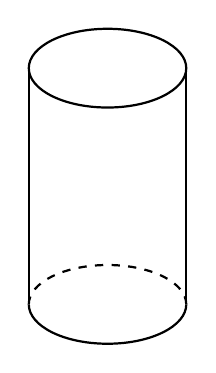
\begin{tikzpicture}[scale=0.5]
    \draw[thick] (0,0) ellipse (2cm and 1cm);
    \draw[thick] (-2,0) to (-2,-6);
    \draw[thick] (2,0) to (2,-6);
    \begin{scope}[shift={(0,-6)}]
      \draw[thick,dashed] (0:2cm and 1cm) arc (0:180:2cm and 1cm);
      \draw[thick] (180:2cm and 1cm) arc (180:360:2cm and 1cm);
    \end{scope}
  \end{tikzpicture}
\] (that's supposed to look like a pipe!) and \[
  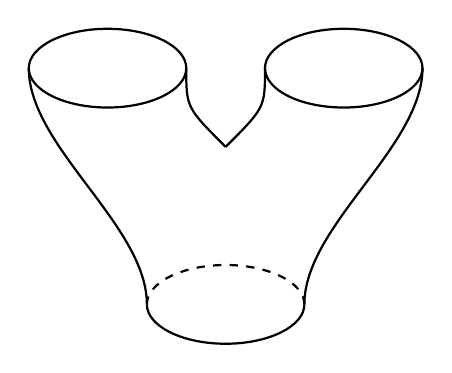
\begin{tikzpicture}[scale=0.5]
    \draw[thick] (-3,0) ellipse (2cm and 1cm);
    \draw[thick] (3,0) ellipse (2cm and 1cm);
    \draw[thick] (-5,0) .. controls (-5,-2) and (-2,-4) .. (-2,-6);
    \draw[thick] (5,0) .. controls (5,-2) and (2,-4) .. (2,-6);
    \draw[thick] (-1,0) .. controls (-1,-1) .. (0,-2);
    \draw[thick] (1,0) .. controls (1,-1) .. (0,-2);
    \begin{scope}[shift={(0,-6)}]
      \draw[thick,dashed] (0:2cm and 1cm) arc (0:180:2cm and 1cm);
      \draw[thick] (180:2cm and 1cm) arc (180:360:2cm and 1cm);
    \end{scope}
  \end{tikzpicture}
\] --- that is, a cylinder and a ``trinion'' (or upside-down pair of
pants) --- we can combine them either ``horizontally'' like this: \[
  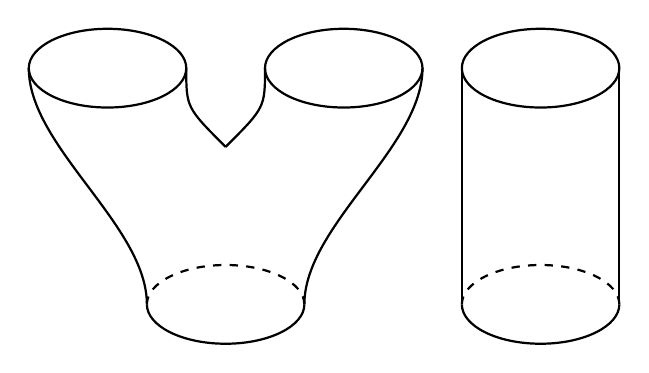
\begin{tikzpicture}[scale=0.5]
    \begin{scope}[shift={(8,0)}]
      \draw[thick] (0,0) ellipse (2cm and 1cm);
      \draw[thick] (-2,0) to (-2,-6);
      \draw[thick] (2,0) to (2,-6);
      \begin{scope}[shift={(0,-6)}]
        \draw[thick,dashed] (0:2cm and 1cm) arc (0:180:2cm and 1cm);
        \draw[thick] (180:2cm and 1cm) arc (180:360:2cm and 1cm);
      \end{scope}
    \end{scope}
    \draw[thick] (-3,0) ellipse (2cm and 1cm);
    \draw[thick] (3,0) ellipse (2cm and 1cm);
    \draw[thick] (-5,0) .. controls (-5,-2) and (-2,-4) .. (-2,-6);
    \draw[thick] (5,0) .. controls (5,-2) and (2,-4) .. (2,-6);
    \draw[thick] (-1,0) .. controls (-1,-1) .. (0,-2);
    \draw[thick] (1,0) .. controls (1,-1) .. (0,-2);
    \begin{scope}[shift={(0,-6)}]
      \draw[thick,dashed] (0:2cm and 1cm) arc (0:180:2cm and 1cm);
      \draw[thick] (180:2cm and 1cm) arc (180:360:2cm and 1cm);
    \end{scope}
  \end{tikzpicture}
\] or ``vertically'' like this: \[
  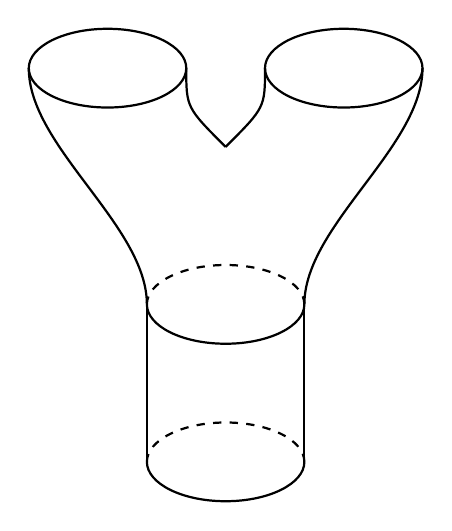
\begin{tikzpicture}[scale=0.5]
    \draw[thick] (-3,0) ellipse (2cm and 1cm);
    \draw[thick] (3,0) ellipse (2cm and 1cm);
    \draw[thick] (-5,0) .. controls (-5,-2) and (-2,-4) .. (-2,-6);
    \draw[thick] (5,0) .. controls (5,-2) and (2,-4) .. (2,-6);
    \draw[thick] (-1,0) .. controls (-1,-1) .. (0,-2);
    \draw[thick] (1,0) .. controls (1,-1) .. (0,-2);
    \begin{scope}[shift={(0,-6)}]
      \draw[thick,dashed] (0:2cm and 1cm) arc (0:180:2cm and 1cm);
      \draw[thick] (180:2cm and 1cm) arc (180:360:2cm and 1cm);
    \end{scope}
    \draw[thick] (-2,-6) to (-2,-10);
    \draw[thick] (2,-6) to (2,-10);
    \begin{scope}[shift={(0,-10)}]
      \draw[thick,dashed] (0:2cm and 1cm) arc (0:180:2cm and 1cm);
      \draw[thick] (180:2cm and 1cm) arc (180:360:2cm and 1cm);
    \end{scope}
  \end{tikzpicture}
\]

Corresponding to each spacetime we have a ``time evolution operator''
--- a linear operator that describes how states going in one end pop out
the other, ``evolved in time''. And corresponding to horizontal and
vertical composition of spacetimes we have two ways to compose
operators: horizontal composition usually being called ``tensor
product'', and vertical composition being called simply ``composition''.
These two ways satisfy some compatibility conditions, as well.

Now if one has read a bit about \(n\)-categories and/or ``extended''
topological quantum field theories, one already knows that this is just
the tip of the iceberg. If we allow ourselves to cut spacetimes into
smaller bits --- e.g., pieces with ``corners'', such as tetrahedra or
their higher-dimensional kin --- one gets more possible ways of
composing operators, and more compatibility conditions. These become
algebraically rather sophisticated, but luckily, there is a huge amount
of evidence that existing TQFTs extend to more sophisticated structures
of this sort, through a miraculous harmony between algebra and topology.

This leads to some interesting new concepts when it comes to the
physical interpretation of extended TQFTs. As Crane described in his
talk (see also his papers listed in \protect\hyperlink{week2}{``Week
2''}, \protect\hyperlink{week23}{Week 23} and
\protect\hyperlink{week56}{Week 56}), in a 4-dimensional extended TQFT
one expects the following sort of thing. If we think of an ``observer''
as a 3-manifold with boundary --- imagine a person being the 3-manifold
and his skin being the boundary, if one likes --- the extended TQFT
should assign to his boundary a ``Hilbert category'' or ``2-Hilbert
space''. This is the categorical analog of a Hilbert space. In other
words, just as a Hilbert space is a \emph{set} in which you can
\emph{sum} things and \emph{multiply} them by \emph{complex numbers},
and get \emph{complex numbers} by taking \emph{inner products} of
things, a 2-Hilbert space is an analogous structure in which every term
surrounded by asterisks is replaced by its analog one step up the
categorical ladder. This means: \[
  \begin{aligned}
    \text{set} &\to \text{category}
  \\\text{sum} &\to \text{direct sum}
  \\\text{multiply} &\to \text{tensor}
  \\\text{complex numbers} &\to \text{vector spaces}
  \\\text{inner products} &\to \text{homs}
  \end{aligned}
\]

There's a good chance that you know the analogy between numbers and
vector spaces: just as you can add numbers and multiply them, you can
take direct sums and tensor products of vector spaces, and many of the
same rules still apply (in a somewhat more sophisticated form, because
laws that were equations are now isomorphisms). A little less familiar
is the analogy between inner products and ``homs''. Given two vectors
\(v\) and \(w\) in a Hilbert space you can take the inner product
\(\langle v,w\rangle\) and get a number; similarly, given two
(finite-dimensional) Hilbert spaces \(V\) and \(W\) you can form
\(\mathrm{hom}(V,W)\) --- that is, the set of all linear maps from \(V\)
to \(W\) --- and get a Hilbert space. The same thing works in any
``2-Hilbert space''.

The most basic example of a 2-Hilbert space would be Hilb, the category
of finite-dimensional Hilbert spaces, but also \(\mathsf{Reps}(G)\), the
category of finite-dimensional unitary representations of a finite
group. (Similar remarks hold for quantum groups at root of unity.) Just
as the inner product is linear in one argument and conjugate-linear in
the other, ``\(\mathrm{hom}\)'' behaves nicely under direct sums in each
argument, but each argument behaves a bit differently under tensor
product, so one can say it's ``linear'' in one and ``conjugate-linear''
in the other.

So anyway, just as in a 4d TQFT a 3-manifold \(M\) determines a Hilbert
space \(Z(M)\), and a 4-manifold \(N\) with boundary equal to \(M\)
determines a vector \(Z(N)\) in \(Z(M)\), something similar happens in
an extended TQFT. (For experts, here I'm really talking about
``unitary'' TQFTs and extended TQFTs --- these are the physically
sensible ones.) Namely, a ``skin of observation'' or 2-manifold \(S\)
determines a 2-Hilbert space \(Z(S)\), and an ``observer'' or 3-manifold
\(M\) with boundary equal to \(S\) determines an object in \(Z(S)\).
Now, given two observers \(M\) and \(M'\) with the same ``skin'' --- for
example, the observer ``you'' and the observer ``everything in the world
except you'' --- one gets two objects \(Z(M)\) and \(Z(M')\) in
\(Z(S)\), so one can form the ``inner product''
\(\mathrm{hom}(Z(M),Z(M'))\), which is a Hilbert space. This is
\emph{your} Hilbert space for describing states of \emph{everything in
the world except you}. Note that we are using the term ``observer'' here
in a somewhat whimsical sense; in particular, every region of space
counts as an observer in this game, so we can flip things around and
form the inner product \(\mathrm{hom}(Z(M'),Z(M))\), which is the
Hilbert space that \emph{everything in the world except you} can use to
describe states of \emph{you}. These two Hilbert spaces, with roles
reversed, are conjugate to each other (using an obvious but perhaps
slightly unfamiliar definition of ``conjugate'' Hilbert space), so
they're pretty much the same.

Now this may at first seem weird, but if you think about it, it becomes
a bit less so. Of course, all of this stuff simply follows from the
notion of a unitary extended TQFT, and whether the actual laws of
physics are given by such a structure is a separate issue. But there is
clearly a lot of relevance to the ``holographic hypothesis'' and Lee
Smolin's more mathematical version of that hypothesis, as sketched in
\protect\hyperlink{week57}{``Week 57''}. The basic idea, there as here,
is that we are concentrating our attention on the things about a system
that can be measured at its boundary, and what we measure there can be
either thought of describing the state of the ``inside'' or dually the
``outside''.

I think if I go out on a limb here, and rhapsodize a bit, the point
might be clearer: but don't take this too seriously. Namely: all of the
stuff you see, hear, and otherwise observe about the world --- which
seems to be ``information about the outside'' --- is also stuff going on
in your brain, hence ``information about the inside''. What this stuff
really is, of course, is \emph{correlations} between the inside and the
outside. This is the reason for the duality between observer and
observed mentioned above. Note: we need not worry here whether or not
there's ``really'' a lot more going on outside than what you observe.
The point is simply that everything \emph{you} observe about what's
going on in the world outside is correlated to stuff that the world
could observe about what is going on in you. (Maybe.)

I should perhaps also add that the mathematicians are getting a bit
behind on the job of developing the ``higher linear algebra'' needed to
support this sort of physics. So it's a bit hard to point to a good
reference for all this 2-Hilbert space stuff. I'm slowly writing a paper
on it, but for now the best sources seem to be Kapranov and Voevodsky's
work on 2-vector spaces:

\begin{enumerate}
\def\labelenumi{\arabic{enumi})}
\setcounter{enumi}{1}
\tightlist
\item
  M. Kapranov and V. Voevodsky, ``2-Categories and Zamolodchikov
  tetrahedra equations'', in \emph{Proc. Symp. Pure Math.} \textbf{56},
  Part 2 (1994), AMS, Providence, pp.~177--260.
\end{enumerate}

(see also \protect\hyperlink{week4}{``Week 4''}) Dan Freed's work on
higher algebraic structures in gauge theory
(\protect\hyperlink{week12}{``Week 12''},
\protect\hyperlink{week48}{``Week 48''}), and David Yetter's new paper:

\begin{enumerate}
\def\labelenumi{\arabic{enumi})}
\setcounter{enumi}{2}
\tightlist
\item
  David Yetter, ``Categorical linear algebra: a setting for questions
  from physics and low-dimensional topology'', Kansas U. preprint,
  available as \texttt{http://math.ucr.edu/home/baez/yetter.pdf} and
  \texttt{http://math.ucr.edu/home/baez/yetter.ps}
\end{enumerate}

This treats 2-vector spaces in a very beautiful way, but not 2-Hilbert
spaces. Definitely worth reading for anyone interested in this sort of
thing!

While visiting Porto, I managed somehow to miss talking to Eugenia Cesar
de Sa, which was really a pity because she was the one who developed the
way of describing 4-manifolds that Broda (see
\protect\hyperlink{week9}{``Week 9''}, \protect\hyperlink{week10}{``Week
10''}) used to construct a 4-dimensional TQFT. This TQFT was later shown
by Roberts (see \protect\hyperlink{week14}{``Week 14''}) to be
isomorphic to that described by Crane and Yetter using a state sum model
--- i.e., by a discrete analog of a path integral in which one chops
spacetime up into 4-dimensional ``hypertetrahedra'' (better known as
4-simplices!), labels their 2d and 3d faces by spins, and sums over
labellings. Her work is cited in the Broda reference in
\protect\hyperlink{week17}{``Week 17''}, but I managed luckily to get a
copy of her thesis:

\begin{enumerate}
\def\labelenumi{\arabic{enumi})}
\setcounter{enumi}{3}
\tightlist
\item
  Eugenia Cesar de Sa, \emph{Automorphisms of 3-manifolds and
  representations of 4-manifolds}, Ph.D.~thesis, University of Warwick,
  1977.
\end{enumerate}

This should let me learn more about 4-dimensional topology, a
fascinating subject on which I'm woefully ignorant.

One reason why Broda's work, and thus de Sa's, is interesting to me, is
that people have suspected for a while that the Crane-Yetter-Broda
theory, which is constructed purely combinatorially, is isomorphic to BF
theory with cosmological term. BF theory (see
\protect\hyperlink{week36}{``Week 36''}) is a 4-dimensional field theory
that can be described starting from a Lagrangian in the traditional
manner of physics. The theory ``with cosmological term'' can be regarded
as a baby version of quantum gravity with nonzero cosmological constant,
a baby version having only one state, the ``Chern-Simons state''. As I
discussed in \protect\hyperlink{week56}{``Week 56''}, it's this
Chern-Simons state that plays a key role in Smolin's attempt to
``exactly solve'' quantum gravity. Thus I suspect that BF theory is a
good thing to understand really well. Recently I showed in

\begin{enumerate}
\def\labelenumi{\arabic{enumi})}
\setcounter{enumi}{4}
\tightlist
\item
  John Baez, ``4-dimensional BF theory with cosmological term as a
  topological quantum field theory'', available as
  \href{http://xxx.lanl.gov/abs/q-alg/9507006}{\texttt{q-alg/9507006}}.
\end{enumerate}

that the Crane-Yetter-Broda theory is indeed isomorphic as a TQFT to a
certain BF theory. With a bit more work, this should give us a state sum
model for the BF theory that's a baby version of quantum gravity in 4
dimensions. This should come in handy for studying Smolin's hypothesis
and its ramifications.

\begin{enumerate}
\def\labelenumi{\arabic{enumi})}
\setcounter{enumi}{5}
\tightlist
\item
  Timothy Porter, ``TQFTs from homotopy \(n\)-types'', University of
  Wales, Bangor preprint, available at
  \texttt{http://www.bangor.ac.uk/\textasciitilde{}mas013/preprint.html}
\end{enumerate}

The Dijkgraaf-Witten model is an n-dimensional TQFT one gets from a
finite group \(G\). It's given by a really simple state sum model. Chop
your manifold into simplices; then the allowed ``states'' are just
labellings of the edges with elements of \(G\) subject to the constraint
that the product around any triangle is \(1\). You can think of a
labelling as a kind of ``connection'' that tells you how to parallel
transport along the edges, and the constraint says the connection is
flat. Expectation values of physical observables are then computed as
sums over these states. In fact, this TQFT is a baby version of BF
theory \emph{without} cosmological constant. A toy model of a toy model
of quantum gravity, in other words: the classical solutions of BF theory
without cosmological constant are just flat connections on some G-bundle
where G is a Lie group, while the Dijkgraaf-Witten model does something
similar for a finite group.

In a previous paper (see \protect\hyperlink{week54}{``Week 54''}) Porter
studied the Dijkgraaf-Witten model and a generalization of it due to
Yetter that allows one to label faces with things too\ldots{} one can
think of this generalization as allowing ``curvature'', because the
product of elements of G around a triangle need no longer be \(1\);
instead, it's something determined by the labelling of the face.

\begin{enumerate}
\def\labelenumi{\arabic{enumi})}
\setcounter{enumi}{6}
\tightlist
\item
  David Yetter, ``TQFTs from homotopy 2-types'', \emph{Journal of Knot
  Theory and its Ramifications} \textbf{2} (1993), 113--123.
\end{enumerate}

In his new paper Porter takes this idea to its logical conclusion and
constructs analogous theories that allow labellings of simplices in any
dimension. Technically, the input data is no longer just a finite group,
but a finite simplicial group \(G\).

What's a simplicial group? It's a wonderful thing; using the
``internalization'' trick I've referred to in some previous Finds, all I
need to say is that it's a simplicial object in the category of groups.
A simplicial set is a bunch of sets, one for each natural number,
together with a bunch of ``face'' and ``degeneracy'' maps satisfying the
same laws that the face and degeneracy maps do for a simplex. (Students
of singular or simplicial homology will know what I'm talking about.)
Similarly, a simplicial group is a bunch of \emph{groups}, together with
a bunch of of ``face'' and ``degeneracy'' \emph{homomorphisms}
satisfying the same laws.

A triangulated manifold gives a simplicial set in an obvious way, and
from any simplicial set one can obtain a simplicial groupoid (like a
simplicial group, but with groupoids instead!) called its ``loop
groupoid''. The sort of labellings Porter considers are homomorphisms
from this simplicial groupoid to the given simplicial group G.

I will refrain from trying to say what all this has to do with homotopy
\(n\)-types. Nonetheless, from a pure mathematics point of view, that's
the most exciting aspect of the whole business! Part of the puzzle about
TQFTs is their relation to traditional algebraic topology (and
not-so-traditional algebraic topology like nonabelian cohomology,
\(n\)-stacks, etc.), and this work serves as a big clue about that
relationship.

\begin{center}\rule{0.5\linewidth}{0.5pt}\end{center}
\hypertarget{week59}{%
\section{August 3, 1995}\label{week59}}

\begin{quote}
\emph{As you crack your eyes one morning your reason is assaulted by a}
\emph{strange sight. Over your head, humming quietly, there floats a}
\emph{monitor, an ethereal otherworldly screen on which is written a
curious} \emph{message. "I am the Screen of ultimate Truth. I am bulging
with} \emph{information and ask nothing better than to be allowed to
impart it."}
\end{quote}

It would be nice if more math books started with something
attention-grabbing like this. In fact, it appears near the beginning of

\begin{enumerate}
\def\labelenumi{\arabic{enumi})}
\tightlist
\item
  Geoffrey M. Dixon, \emph{Division Algebras: Octonions, Quaternions,
  Complex Numbers and the Algebraic Design of Physics}, Springer Verlag,
  1994.
\end{enumerate}

Dixon is convinced that the details of the Standard Model of particle
interactions can be understood better by taking certain mathematical
structures very seriously. There are very few algebras over the reals
where we can divide by nonzero elements: if we demand associativity and
commutativity, just the reals themselves and the complex numbers. If we
drop the demand for commutativity, we also get a 4-dimensional algebra
called the quaternions, invented by Hamilton. If in addition we drop the
demand for associativity, and ask only that our algebra be
``alternative'', we also get an 8-dimensional algebra called the
octonions, or Cayley numbers. (I'll say what ``alternative'' means in
\protect\hyperlink{week61}{``Week 61''}) Clearly these are very special
structures, and also clearly they play an important role in
physics\ldots{} or do they?

Well, few people doubt that the real numbers are fundamental to physics
(though some advocates of the discrete might prefer the integers), and
with emergence of quantum theory, if not sooner, the basic role of the
complex numbers also became clear. Hamilton discovered the quaternions
in the 1800s, and used them to formulate a beautiful theory of rotations
in 3-dimensional space. They fell out of favor somewhat when the vectors
of Gibbs proved simpler for many purposes, but their deeper importance
became clear when people started studying spin: indeed, the Pauli
matrices so important in physics are closely related to the quaternions,
and it is the group of unit quaternions, \(SU(2)\), rather than the
group of rotations in 3d space, \(SO(3)\), which turns out to be the
symmetry group whose different representations correspond to particles
of different spin. But what about the octonions?

Well, there are not too many places in physics yet where the octonions
reach out and grab one with the force the reals, complexes, and
quaternions do. But they are certainly out there, they have a certain
beauty to them, and they are the natural stopping-point of a certain
finite sequence of structures, so it is natural for people of a certain
temperament to believe that they are there for a reason. Dixon makes a
passionate case for this in the beginning of his book.

Suppose you were confronted with the Screen of Truth. What would you ask
it? Dixon, being a physicist, naturally fantasizes asking it why the
universe is the way it is! What kind of answer could this possibly have?
Perhaps there is only one consistent way for things to be, and
mathematics, with its unique and beautiful structures that are pure
expressions of logical necessity, is trying to tell us something about
this?

On the one hand this seems outrageous\ldots{} especially to the
hard-nosed pragmatist or empiricist in us. It seems old-fashioned,
naive, and too good to be true. On the other hand, the universe
\emph{is} outrageous! It's outrageous that it exists in the first place,
and doubly outrageous that it has the particular physical laws it does
and no others. It has only been through the old-fashioned, naive belief
that we can understand it using mathematics that we discovered what we
have of its physical laws. So maybe eventually we \emph{will} see that
the basic structures of mathematics determine, in some mysterious sense,
all the basic laws of physics. Or maybe we won't. In either case, there
is a long way yet to go. As Dixon's Screen of Truth comments, before it
departs:

\begin{quote}
``Do you believe that were I to explain as much of what I know as you''
``could comprehend that you would recognize it, that you would say, oh''
``yes, this is but an extension of what we have already done, and
though'' ``the mathematics is broader, the principles deeper, I am not
surprised?'' ``Do you think you have asked even a fraction of the
questions you need'' ``to ask?''
\end{quote}

Anyway, it is at least worth considering all the beautiful mathematical
structures one runs into for their potential importance. For example,
the octonions.

In order to write this week's Finds, I needed to learn a little about
the octonions. I wanted some good descriptions of the octonions, that
hopefully would ``explain'' them or at least make them easy to remember.
So I asked for help on sci.physics.research, and I got some help from
Greg Kuperberg, Ezra Getzler, Matthew Wiener, and Alexander Vlasov.
After a while Geoffrey Dixon got wind of this and referred me to his
work! I'll probably talk to him later this summer when I go back to
Cambridge Massachusetts, and hopefully I'll learn more about octonions
and the like.

But for now let me just give a quick beginner's introduction to the
octonions. A lot of this appears in

\begin{enumerate}
\def\labelenumi{\arabic{enumi})}
\setcounter{enumi}{1}
\tightlist
\item
  William Fulton and Joe Harris, \emph{Representation Theory --- a First
  Course}, Springer Verlag, Berlin, 1991.
\end{enumerate}

I should add that this book is a very good place to learn about Lie
groups, Lie algebras, and their representations\ldots{} I wish I had
taken a course based on this book when I was in grad school!

Let's start with the real numbers. Then the complex number \[a+bi\] can
be thought of as a pair \[(a,b)\] of real numbers. Addition is done
component-wise, and multiplication goes like this:
\[(a,b)(c,d) = (ac - db,da + bc)\] We can also define the conjugate of a
complex number by \[(a,b)^* = (a,-b).\] Now that we have the complex
numbers, we can define the quaternions in a similar way. A quaternion
can be thought of as a pair \[(a,b)\] of complex numbers. Addition is
component-wise and multiplication goes like this
\[(a,b)(c,d) = (ac - d^*b, da + bc^*)\] This is just like how we defined
multiplication of complex numbers, but with a couple of conjugates
(\({}^*\)'s) thrown in. To emphasize how similar the two multiplications
are, we could have included the conjugates in the first formula, since
the conjugate of a real number is just itself.

We can also define the conjugate of a quaternion by
\[(a,b)^* = (a^*,-b).\] The game continues! Now we can define an
octonion to be a pair of quaternions; as before, we add these
component-wise and multiply them as follows:
\[(a,b)(c,d) = (ac - d^*b, da + bc^*).\] One can also define the
conjugate of an octonion by \[(a,b)^* = (a^*,-b).\] Why do the real
numbers, complex numbers, quaternions and octonions have multiplicative
inverses? I take it as obvious for the real numbers. For the complex
numbers, you can check that \[(a,b)^* (a,b) = (a,b) (a,b)^* = K (1,0)\]
where \(K\) is a real number called the ``norm squared'' of \((a,b)\).
The multiplicative identity for the complex numbers is \((1,0)\). This
means that the multiplicative inverse of \((a,b)\) is \((a,b)^*/K\). You
can check that the same holds for the quaternions and octonions!

This game of getting new algebras from old is called the
``Cayley-Dickson'' construction. Of course, the fun we've had so far
should make you want to keep playing this game and develop a
16-dimensional algebra, the ``hexadecanions,'' consisting of pairs of
octonions equipped with the same sort of multiplication law. What do you
get? Why aren't there multiplicative inverses anymore? I haven't
checked, because this is my summer vacation! I am learning about
octonions just for fun, since I just finished writing some rather
technical papers, and my idea of fun does not presently include
multiplying two hexadecanions together to see why the norm-squared law
\((a,b) (a,b)^* = (a,b)^* (a,b) = K (1,0)\) breaks down. But I'm sure
someone out there will enjoy doing this\ldots{} and I'm sure someone
else out there has already done it! So they should let me know what
happens. There is something out there called ``Pfister forms'', which I
think might be related.

{[}Toby Bartels did some nice work on hexadecanions in response to the
above challenge, which appears at the end of this article.{]}

Now if we unravel the above definition of quaternions, by writing the
quaternion \((a+bi,c+di)\) as \(a+bi+cj+dk\), we see that the
multiplication law is \[i^2 = j^2 = k^2 = -1,\] and
\[ij = -ji = k, \quad jk = -kj = i, \quad ki = -ik = j.\]

For more about the inner meaning of these rules, see
\protect\hyperlink{week5}{``Week 5''}. Similarly, we can unravel the
above definition of octonions by writing the octonion
\((a+bi+cj+dk,e+fi+gj+hk)\) as
\[a + b e_1 + c e_2 + d e_3 + e e_4 + f e_5 + g e_6 + h e_7.\] Note:
since mathematicians are very impersonal, they usually call these seven
dwarves \(e_1,\ldots,e_7\) instead of Sleepy, Grumpy, etc. as in the
Disney movie. Any one of these 7 guys times himself is \(-1\). Also, any
two distinct ones anticommute; for example, \(e_3 e_7 = -e_7 e_3\).
There is a nice way to remember how to multiply them using the ``Fano
plane''. This is a projective plane with 7 points, where by a
``projective plane'' I mean that any two points determine an abstract
sort of ``line'', which in this case consists of just 3 points, and any
two lines intersect in a point. It looks like this:
\[![](../images/fano.jpg)\]

The ``lines'' are the 3 edges of the big triangle, the 3 lines going
through a vertex, the center and the midpoint of the opposite edge, and
the circle including \(e_1\), \(e_2\), and \(e_3\). All the ``lines''
are cyclically ordered, and that tells you how to multiply the seven
dwarves. For example, the line that's actually a circle goes clockwise,
so \(e_1 e_2 = e_4\), \(e_2 e_4 = e_1\), and \(e_4 e_1 = e_2\). The
lines that are edges of the big triangle also point clockwise, so for
example \(e_5 e_2 = e_3\), and cyclic permutations thereof, and
\(e_6 e_3 = e_4\). The lines that go through the center point from the
vertex to the midpoint of the opposite edge, so for example
\(e_3 e_7 = e_1\). I hope that made sense; you can work it out yourself,
of course.

My convention for numbering the seven dwarves in the picture above is
\emph{completely arbitrary}, so don't bother remembering it --- make up
your own if you prefer! The convention I chose looks sort of weird at
first, but it has a couple of endearing features:

\begin{itemize}
\tightlist
\item
  Index cycling: if \(e_i e_j = e_k\), then
  \(e_{i+1} e_{j+1} = e_{k+1}\).
\item
  Index doubling: if \(e_i e_j = e_k\), then \(e_{2i} e_{2j} = e_{2k}\).
\end{itemize}

Here we add and multiply \(\mod 7\). Index doubling corresponds to
rotating the Fano plane.

So those are the octonions in a nutshell. I should say a bit about how
they relate to triality for \(SO(8)\), the exceptional Lie group
\(G_2\), the group \(SU(3)\) which is so important in the study of the
strong force, and to lattices like \(E_8\), \(\Lambda 16\) and the Leech
lattice. But I will postpone that; for now you can consult Fulton and
Harris, and also various papers by Dixon:

\begin{enumerate}
\def\labelenumi{\arabic{enumi})}
\setcounter{enumi}{2}
\item
  Geoffrey Dixon, ``Octonion X-product orbits'', preprint available as
  \href{http://xxx.lanl.gov/abs/hep-th/9410202}{\texttt{hep-th/9410202}}.

  ``Octonion X-product and E\_8 lattices'', preprint available as
  \href{http://xxx.lanl.gov/abs/hep-th/9411063}{\texttt{hep-th/9411063}}.

  ``Octonions: \(E_8\) lattice to \(\Lambda 16\)'', preprint available
  as
  \href{http://xxx.lanl.gov/abs/hep-th/9501007}{\texttt{hep-th/9501007}}.

  ``Octonions: invariant representation of the Leech lattice'', preprint
  available as
  \href{http://xxx.lanl.gov/abs/hep-th/9504040}{\texttt{hep-th/9504040}}.

  ``Octonions: invariant Leech lattice exposed'', preprint available as
  \href{http://xxx.lanl.gov/abs/hep-th/9506080}{\texttt{hep-th/9506080}}.
\end{enumerate}

I am not presently in a position to assess these papers or Dixon's work
relating division algebras and the Standard Model, but hopefully
sometime I will be able to say a bit more.

Let me wrap up by saying a bit about the Leech lattice. As described in
my review of Conway and Sloane's book (\protect\hyperlink{week20}{``Week
20''}, there is a wonderful branch of mathematics that studies the
densest ways of packing spheres in n dimensions. Most of the results so
far concern lattice packings, packings in which the centers of the
spheres form a subset of \(\mathbb{R}^n\) closed under addition and
scalar multiplication by integers. When \(n = 8\), the densest known
packing is given by the so-called \(E_8\) lattice. In
\protect\hyperlink{week20}{``Week 20''} I described how to get this
lattice using the quaternions and the icosahedron. Briefly, it goes as
follows. The group of rotational symmetries of the icosahedron (not
counting reflections) is a subgroup of the rotation group \(SO(3)\)
containing 60 elements. As mentioned above, \(SO(3)\) has as a double
cover the group \(SU(2)\) of unit quaternions. So there is a 120-element
subgroup of \(SU(2)\) consisting of elements that map to elements of
\(SO(3)\) that are symmetries of the icosahedron. Now form all integer
linear combinations of these 120 special elements of \(SU(2)\). We get a
subring of the quaternions known as the "icosians'\,'.

We can think of icosians as special quaternions, but we can also think
of them as special vectors in \(\mathbb{R}^8\), as follows. Every
icosian is of the form
\[(a + \sqrt{5} b) + (c + \sqrt{5} d)i + (e + \sqrt{5} f)j + (g + \sqrt{5} h)k\]
with \(a,b,c,d,e,f,g,h\) rational --- but not all rational values of
\(a,\ldots,h\) give icosians. The set of all vectors
\(x = (a,b,c,d,e,f,g,h)\) in \(\mathbb{R}^8\) that correspond to
icosians in this way is the \(E_8\) lattice!

The Leech lattice is the densest known packing in 24 dimensions. It has
all sorts of remarkable properties. Here is an easy way to get ones
hands on it. First consider triples of icosians \((x,y,z)\). Let \(L\)
be the set of such triples with \[x = y = z \mod h\] and
\[x + y + z = 0 \mod h^*\] where \(h\) is the quaternion
\((-\sqrt{5} + i + j + k)/2\). Since we can think of an icosian as a
vector in \(\mathbb{R}^8\), we can think of \(L\) as a subset of
\(\mathbb{R}^{24}\). It is a lattice, and in fact, it's the Leech
lattice! I have a bit more to say about the Leech lattice in
\protect\hyperlink{week20}{``Week 20''}, but the real place to go for
information on this beast is Conway and Sloane's book. It turns out to
be related to all sorts of other "exceptional'\,' algebraic structures.
People have found uses for many of these in string theory, so if string
theory is right, maybe they are important in physics. Personally, I want
to understand them more deeply as pure mathematics before worrying too
much about their applications to physics.

\begin{center}\rule{0.5\linewidth}{0.5pt}\end{center}

Here is what Toby Bartels wrote:

\begin{quote}
From: Toby Bartels Subject: Re: why hexadecanions have no inverses To:
John Baez Date: Sun, 20 Aug 1995
\end{quote}

\begin{quote}
I spent a couple days thinking about why hexadecanions have no inverses,
and the first thing I want to say about it is that they do. However,
these inverses are of limited applicability, because the hexadecanions
are not a division algebra. A division algebra allows you to conclude,
given \(x y = 0\), that \(x\) or \(y\) is \(0\). If your algebra has
inverses, you might try to multiply this equation by the inverse of
\(x\) or \(y\) (whichever one isn't \(0\)) to prove the other is \(0\),
but this only works if the algebra is associative. Since the octonions
and hexadecanions aren't associative, there's no reason (yet) to think
either of these is a division algebra. It turns out that the octonions
are a division algebra, despite not being associative, but the
hexadecanions aren't.

Why aren't the hexadecanions a division algebra? Because the real
numbers aren't of characteristic 2. Allow me to explain.

I will prove below that the \(2^n\) onions are a division algebra only
if the \(2^{n-1}\) onions are associative. So, the question becomes: why
aren't the octonions associative? Well, I've found a proof that \(2^n\)
onions are associative only if \(2^{n-1}\) onions are commutative. So,
why aren't the quaternions commutative? Again, I have a proof that
\(2^n\) onions are commutative only if \(2^{n-1}\) onions equal their
own conjugates. So, why don't the complex numbers equal their own
conjugates? I have a proof that \(2^n\) onions do equal their own
conjugates, but it works only if the \(2^{n-1}\) onions are of
characteristic 2. The real numbers are not of characteristic 2, so the
complex numbers don't equal their own conjugates, so the quaternions
aren't commutative, so the octonions aren't associative, so the
hexadecanions aren't a division algebra.

I require a few identities about conjugates that hold for all \(2^n\)
onions: \((x^*)^* = x\), \((x + y)^* = x^* + y^*\), and
\((x y)^* = y^* x^*\). (If these identities are reminiscent of
identities for transposes of matrices, it is no coincidence.) I will
prove these by induction. That is, if an identity holds for \(2^{n-1}\)
onions, I show it holds for \(2^n\) onions. Since they hold trivially
for the reals (\(n = 0\)), they hold for all.

\[((a, b)^*)^* = (a^*, -b)^* = ((a^*)^*, -(-b)).\] By the induction
hypothesis and the nature of addition (an Abelian group),
\[((a^*)^*, -(-b)) = (a, b).\]
\[((a, b) + (c, d))^* = (a + c, b + d)^* = ((a + c)^*, -(b + d)).\] By
the induction hypothesis and addition again,
\[((a + c)^*, -(b + d)) = (a^* + c^*, -b + -d) = (a^*, -b) + (c^*, -d) = (a, b)^* + (c, d)^*.\]

The next proof needs the distribution of multiplication over addition.
\[(a, b) ((c, d) + (e, f)) = (a, b) (c + e, d + f) = (a (c + e) - (d + f)^* b, (d + f) a + b (c + e)^*).\]
By the induction hypothesis and the identity immediately above, \[
  \begin{gathered}
    (a (c + e) - (d + f)^* b, (d + f) a + b (c + e)^*)
  \\= (a c + a e - d^* b - f^* b, d a + f a + b c^* + b e^*)
  \\= (a c - d^* b, d a + b c^*) + (a e - f^* b, f a + b e^*)
  \\= (a, b) (c, d) + (a, b) (e, f).
  \end{gathered}
\] Also, \[
  \begin{gathered}
    ((a, b) + (c, d)) (e, f)
  \\= (a + c, b + d) (e, f)
  \\= ((a + c) e - f^* (b + d), f (a + c) + (b + d) e^*).
  \end{gathered}
\] By the induction hypothesis again, \[
  \begin{gathered}
    ((a + c) e - f^* (b + d), f (a + c) + (b + d) e^*)
  \\= (a e + c e - f^* b - f^* d, f a + f c + b e^* + d e^*)
  \\= (a e - f^* b, f a + b e^*) + (c e - f^* d, f c + d e^*)
  \\= (a, b) (e, f) + (c, d) (e, f).
  \end{gathered}
\]

\[((a, b) (c, d))^* = (a c - d^* b, d a + b c^*)^* = ((a c - d^* b)^*, -(d a + b c^*)).\]
Using the induction hypothesis and each of the above identities, \[
  \begin{gathered}
    ((a c - d^* b)^*, -(d a + b c^*))
  \\= (c^* a^* - (-b)^* (-d), -d a + (-b) c^*)
  \\= (c^*, -d) (a^*, -b)
  \\= (c, d)^* (a, b)^*.
  \end{gathered}
\]

In light of the above identities, if I ever come across, say,
\((x y^* + z)^*\), I'll simply write \(y x^* + z^*\) without a moment's
hesitation.

Since inductive proofs have been so useful, I'll use one to prove that
\(2^n\) onions always have inverses. First, I'll extend the method in
John's article, beginning with an inductive proof that \(x x^* = x^* x\)
is real. \[(a, b) (a, b)^* = (a, b) (a^*, -b) = (a a^* + b^* b, 0),\]
and \[(a, b)^* (a, b) = (a^*, -b) (a, b) = (a^* a + b^* b, 0).\] The
inductive hypothesis states that both \(a^* a = a a^*\) and \(b^* b\)
are real, so \((a, b) (a, b)^* = (a, b)^* (a, b)\) is real. Since the
sum of a positive real and a nonnegative real is positive, I can take
this as a proof by induction that \(x x^* = x^* x\) is not only real,
but is also positive unless \(x = 0\) (which will be important). All you
have to do now is check that these things are true of the \(2^0\)
onions, and they are, quite trivially (since the \(2^0\) onions are the
reals).

Since the \(2^n\) onions are always a vector space over the reals (as
mentioned in John's article),
\[x (x^* / (x x^*)) = (x x^*) / (x x^*) = 1.\] Since one can always
divide by the real \(x x^*\), the inverse of \(x\) is \(x^* / (x x^*)\)
in any \(2^n\) onion algebra.

To continue with the streak of inductive proofs, I will now try to prove
that the \(2^n\) onions are always a division algebra. (I will fail.)
Assume \[0 = (0, 0) = (a, b) (c, d) = (a c - d^* b, d a + b c^*).\] This
gives the system of equations \[a c - d^* b = 0 = d a + b c^*.\]
Multiplying,
\[(a c) c^* - (d^* b) c^* = 0 c^* = 0 = d^* 0 = d^* (d a) + d^* (b c^*).\]
If \(2^{n-1}\) onions are associative, I can add the equations to get
\[a (c c^*) + (d^* d) a = 0.\] Since \(c c^*\) and \(d^* d\) are real,
they commute with \(a\), and the division algebra nature of \(2^{n-1}\)
onions allows me to conclude that \(c c^* + d^* d = 0\) (which implies
\(c = d = 0\) in light of positive definiteness) or that \(a = 0\) (from
which the original equation gives \(b = 0\)). Thus, the octonions are a
division algebra (since the quaternions are associative), but the
hexadecanions aren't (since the octonions aren't associative).

(If you're reading carefully, you realize that I haven't really proved
that the hexadecanions aren't a division algebra. I've failed to prove
that they are, but that's not the same thing. When I first wrote this, I
wasn't reading carefully; I will return to plug this hole later.)

Thus, the \(2^n\) onions are a division algebra iff the \(2^{n-1}\)
onions are a division algebra and are associative. So, let's try to
prove associativity of \(2^n\) onions by induction. \[
  \begin{gathered}
    ((a, b) (c, d)) (e, f)
  \\= (a c - d^* b, d a + b c^*) (e, f)
  \\= ((a c - d^* b) e - f^* (d a + b c^*), f (a c - d^* b) + (d a + b c^*) e^*)
  \\=((ac)e - (d^* b)e - f^* (da) - f^* (b c^*), f(ac) - f(d^* b) + (da) e^* + (b c^*) e^*).
  \end{gathered}
\] On the other hand, \[
  \begin{gathered}
    (a, b) ((c, d) (e, f))
  \\= (a, b) (c e - f^* d, f c + d e^*)
  \\= (a (c e - f^* d) - (f c + d e^*)^* b, (f c + d e^*) a + b (c e - f^* d)^*)
  \\= (a(ce) - a(f^* d) - (c^* f^*)b - (e d^*)b, (fc)a + (d e^*)a + b(e^* c^*) - b(d^* f)).
  \end{gathered}
\] Assuming the induction hypothesis that \(2^{n-1}\) onions are
associative, these are equal in general iff \(2^{n-1}\) onions also are
commutative.

Thus, \(2^n\) onions are associative iff \(2^{n-1}\) onions are
associative and are commutative. So, let's try to prove commutativity of
\(2^n\) onions by induction.
\[(a, b) (c, d) = (a c - d^* b, d a + b c^*).\] On the other hand,
\[(c, d) (a, b) = (c a - b^* d, b c + d a^*).\] Assuming the induction
hypothesis that \(2^{n-1}\) onions are commutative, these are equal in
general iff \(2^{n-1}\) onions also equal their own conjugates.

Thus, \(2^n\) onions are commutative iff \(2^{n-1}\) onions are
commutative and equal their own conjugates. So, let's try to prove
conjugate equality of \(2^n\) onions by induction. \[(a, b) = (a, b).\]
On the other hand, \[(a, b)^* = (a^*, -b).\] Assuming the induction
hypothesis that \(2^{n-1}\) onions equal their own conjugates, these are
equal in general iff \(2^{n-1}\) onions also have characteristic 2.
(\(b = -b\) means \(0 = b + b = 1 b + 1 b = (1 + 1) b = 2 b\); this is
true in general iff \(0 = 2\), which is what characteristic 2 means.)

Thus, \(2^n\) onions equal their own conjugates iff \(2^{n-1}\) onions
equal their own conjugates and have characteristic 2. Since the reals
don't have characteristic 2, there's no point in trying to prove
anything about that by induction. However, it's a general result that
any algebra has characteristic 2 if it has a superalgebra of
characteristic 2. Since the \(2^n\) onions are all superalgebras of the
reals (which means the reals are always isomorphic to a subset of the
\(2^n\) onions), none of the \(2^n\) onions can have characteristic 2 if
the reals don't.

In summary, the definition of the reals as the complete ordered field,
along with an initial definition that \(x^* = x\) in the reals, allows
trivial proofs that: they form a division algebra, they are associative,
they are commutative, and they equal their own conjugates, but they
don't have characteristic 2. (All of these, in fact, are true of any
ordered field with this definition of conjugate, complete or not.) From
this and the above considerations, the complex numbers form a division
algebra, are associative, and are commutative, but they neither equal
their own conjugates nor have characteristic 2. From this, the
quaternions form a division algebra and are associative, but they
neither are commutative, equal their own conjugates, nor have
characteristic 2. From this, the octonions form a division algebra but
they neither associative, are commutative, equal their own conjugates,
nor have characteristic 2. Finally, the hexadecanions neither form a
division algebra, are associative, are commutative, equal their own
conjugates, nor have characteristic 2.

At this point, I must return to the logical hole I mentioned earlier.
But I want to work with a different algebraic concept than a division
algebra; instead I will use (inspired by Doug Merrit's post to
\texttt{sci.physics.research}) what I guess is called `alternativity',
which says \(x (x y) = (x x) y\). I don't like putting alternativity
into the pattern, since associativity implies alternativity. All the
other properties (commutativity, conjugate equality, characteristic) are
logically independent in general. I'd like to prove that every
associative \(2^n\) onion algebra is alternative, just as I proved every
commutative one was associative, without its having been obvious to
begin with. Well, I will be disappointed even more badly later on.

Taking the conjugate of \(x (x y) = (x x) y\),
\[(y^* x^*) x^* = y^* (x^* x^*),\] so left alternativity implies right
alternativity, for \(2^n\) onions.

I require an additional general identity of \(2^n\) onions. Earlier, I
proved by induction that \(x x^*\) was real, but now I need the reality
of \(x + x^*\). Like everything else, this is proved by induction.
\[(a, b) + (a, b)^* = (a, b) + (a^*, -b) = (a + a^*, 0).\] Thus, if
\(a + a^*\) is real, \((a, b) + (a, b)^*\) is real. Since \(x + x^*\) is
real when \(x\) is real, \(x + x^*\) is real when \(x\) is any \(2^n\)
onion.

Now suppose we're working in an alternative \(2^n\) onion algebra.
\[x (x y) + x^* (x y) = (x + x^*) (x y).\] Since \(x + x^*\) is real, it
associates, so
\[x (x y) + x^* (x y) = ((x + x^*) x) y = (x x) y + (x^* x) y.\] Since
\(x (x y) = (x x) y\), \[x^* (x y) = (x^* x) y,\] which will be needed.

Let's attempt to prove by induction that \(2^n\) onions are always
alternative. \[
  \begin{gathered}
    (a, b) ((a, b) (c, d))
  \\= (a, b) (a c - d^* b, d a + b c^*)
  \\= (a (a c - d^* b) - (d a + b c^*)^* b, (d a + b c^*) a + b (a c - d^* b)^*)
  \\= (a(ac) - a(d^* b) - (a^* d^*)b - (c b^*)b, (da)a + (b c^*)a + b(c^* a^*) - b(b^* d)).
  \end{gathered}
\] Meanwhile, \[
  \begin{gathered}
    ((a, b) (a, b)) (c, d)
  \\= (a a - b^* b, b a + b a^*) (c, d)
  \\= ((aa)c - (b^* b)c - d^* (ba) - d^* (b a^*),d(aa) - d(b^* b) + (ba) c^* + (b a^*) c^*).
  \end{gathered}
\] These are indeed equal in general iff \(2^{n-1}\) onions are
associative.

The last sentence may not be immediately obvious. The induction
hypothesis and its corollaries leave us with
\(x (y z) + (x^* y) z = y (z x) + y (z x^*)\) as a necessary and
sufficient condition. It may not be clear that associativity implies
this, much less vice versa. However, the reality of \(x + x^*\) once
more enters the picture.
\[y (z x) + y (z x^*) = y (z (x + x^*)) = (x + x^*) (y z) = x (y z) + x^* (y z).\]
Thus, the condition becomes
\[x (y z) + (x^* y) z = x (y z) + x^* (y z),\] which is equivalent, in
the general case, to associativity.

To sum up the findings so far: For any n, the \(2^n\) onions form a
vector space over the reals. \(x + x^*\) and \(x x^*\) are real if \(x\)
is any \(2^n\) onion; additionally, \(x x^* = x^* x.\) Every \(2^n\)
onion has an inverse, which is a real multiple of its conjugate.
Conjugation is analogous to matrix transposition in that
\[(x^*)^* = x, (x + y)^* = x^* + y^*, and (x y)^* = y^* x^*.\]
Multiplication distributes over addition every time. For no n do all
\(2^n\) onions equal their own negatives. \(2^{n+1}\) onions equal their
own conjugates iff \(2^n\) onions equal their own conjugates and their
own negatives. all \(2^{n+1}\) onions commute iff all \(2^n\) onions
commute and equal their own conjugates. \(2^{n+1}\) onions are
associative iff \(2^n\) onions are associative and commutative.
\(2^{n+1}\) onions are alternative iff \(2^n\) onions are alternative
and associative. The \(2^n\) onions form a division algebra if they are
alternative.

I will be satisfied if I can prove the converse of the last statement.
In light of the results about alternativity, my original attempt to
prove that division of \(2^n\) onions requires associativity of
\(2^{n-1}\) onions looks even more convincing, (since alternativity of
\(2^{n-1}\) onions can be included in the induction hypothesis), but
it's still not valid. I still haven't shown that, if \(2^{n-1}\) onions
aren't alternative, there must be non0 \(2^n\) onions \(x\) and \(y\)
such that \(x y = 0\). There doesn't seem to be any reason why there
shouldn't be, but there just might happen not to be any. So, despite the
inelegance of it all, in order to prove that the hexadecanions aren't a
division algebra, I'm forced to exhibit non-\(0\) \(x\) and \(y\) such
that \(x y = 0\).

Just playing around, I found \[
  \begin{gathered}
    (e_1, e_4) (-1, e_5)
  \\= (e_1 (-1) - (e_5)* e_4, e_5 e_1 + e_4 (-1)*)
  \\= (-e_1 + e_5 e_4, e_5 e_1 - e_4).
  \end{gathered}
\] Since \(e_5 e_4 = (0, i) (0, 1) = (i, 0) = e_1\) and
\(e_5 e_1 = (0, i) (i, 0) = (0, i* i) = (0, 1) = e_4\),
\[(e_1, e_4) (-1, e_5) = (0, 0) = 0.\]

The \(2^n\) onions can't be a division algebra if the \(2^{n-1}\) onions
aren't. If \(x y = 0\) in the \(2^{n-1}\) onions,
\((x, 0) (y, 0) = (x y, 0) = (0, 0) = 0\). Thus, the octonions and below
are the only \(2^n\) onions to be division algebras. Still, I wish I had
a proof of this that didn't require the ugly brute force use of a
specific counterexample. (This is the interested reader's cue \ldots)

-- Toby
\end{quote}

By the way, in a post to \texttt{sci.physics.research} on November 2,
1999, Ralph Hartley pointed out that even if we start with a field of
characteristic 2, repeatedly applying the Cayley-Dickson construction
will \emph{not} lead to an infinite sequence of division algebras,
because it's not true in this case that if \(x\) is nonzero, \(xx^*\) is
nonzero. The problem is that a field of characteristic 2 can't be an
ordered field.

\begin{center}\rule{0.5\linewidth}{0.5pt}\end{center}
\hypertarget{week60}{%
\section{August 8, 1995}\label{week60}}

The end of a sabbatical is a somewhat sad affair\ldots{} so many plans
one had, and so few accomplished! As I pack my bags to return from
Cambridge England to Cambridge Massachusetts, and then wing my way back
to Riverside, I find I have quite a stack of preprints that I meant to
include in This Week's Finds, but haven't gotten around to yet.

\begin{enumerate}
\def\labelenumi{\arabic{enumi})}
\tightlist
\item
  N. P. Landsman, ``Rieffel induction as generalized quantum
  Marsden-Weinstein reduction'', \emph{Journal of Geometry and Physics}
  \textbf{15} (1995), 285--319.
\end{enumerate}

Marsden-Weinstein reduction, also called symplectic reduction, is the
modern way to deal with constraints in classical mechanics problems.
It's a two-step procedure where first one looks at the subspace of your
phase space on which the constraints vanish, and then a quotient of this
by a certain equivalence relation. For example, if you have a particle
in a plane, its phase space is \(\mathbb{R}^4\), with coordinates
\((x,y,p_x,p_y)\) representing the \(x\) and \(y\) components of the
position and the \(x\) and \(y\) components of the momentum. If we have
a constraint \(x = 0\), Marsden-Weinstein reduction tells us first to
form the subspace of our phase space on which \(x = 0\), and then
quotient by the equivalence relation where two points are equivalent if
they have the same value of \(p_x\). We get down to \(\mathbb{R}^2\),
with coordinates \((y,p_y)\). But Marsden- Weinstein reduction works in
great generality and has become a basic part of the toolkit of
mathematical physics.

What's the quantum analog of Marsden-Weinstein reduction? That's what
this paper is about. Quantum mechanics in the presence of constraints is
a tricky and important business, and there are lots of theories about
how to do it. Gauge theories all have constraints, and so does general
relativity\ldots{} and in quantizing general relativity, the presence of
constraints is what gives rise to the ``problem of time''. (See
\protect\hyperlink{week43}{``Week 43''} for more on this.) What
attracted my attention to this paper is a two-stage procedure for
dealing with contraints, quite analogous to Marsden-Weinstein reduction.
This should shed some interesting light on the problem of time.

\begin{enumerate}
\def\labelenumi{\arabic{enumi})}
\setcounter{enumi}{1}
\item
  T. Ohtsuki, ``Finite type invariants of integral homology 3-spheres'',
  preprint, 1994.

  L. Rozansky, ``The trivial connection contribution to Witten's
  invariant and finite type invariants of rational homology spheres'',
  preprint available as
  \href{http://xxx.lanl.gov/abs/q-alg/9504015}{\texttt{q-alg/9505015}}.

  Stavros Garoufalidis, ``On finite type 3-manifold invariants I'', MIT
  preprint, 1995.

  Stavros Garoufalidis and Jerome Levine, ``On finite type 3-manifold
  invariants II'', MIT preprint, June 1995. (Garoufalidis is at
  \texttt{stavros@math.mit.edu}, and Levine is at
  \texttt{levine@max.math.brandeis.edu}.)

  Ruth J. Lawrence, ``Asymptotic expansions of Witten-Reshetikhin-Turaev
  invariants for some simple 3-manifolds'', to appear in \emph{Jour.
  Math. Physics}.
\end{enumerate}

Chern-Simons theory gives invariant of links in \(\mathbb{R}^3\), which
are functions of Planck's constant \(\hbar\), and if one expands them as
power series in h, the coefficients are link invariants with special
properties, which one summarizes by calling them ``Vassiliev
invariants'' or ``invariants of finite type''. (See
\protect\hyperlink{week3}{``Week 3''} for more.) But the partition
function of Chern-Simons theory on a compact oriented 3-manifold is also
interesting; it's an invariant of the 3-manifold defined for certain
values of \(\hbar\). (Often instead one thinks of it instead as a
function of a quantity \(q\), the limit \(q \to 1\) corresponding to the
limit \(\hbar \to 0\).)

Recently people have studied the partition function of special
3-manifolds called homology spheres, which have the same homology as
\(S^3\). (People have looked at both integral and rational homology
spheres.) After a bit of subtle fiddling, one can extract from the
partition function of a homology sphere a power series in
\[\hbar' = q - 1,\] and the coefficients of the powers of \(\hbar'\)
have been conjectured by Rozansky to have nice properties which one may
summarize by calling them ``finite type'' invariants, in analogy to the
link invariant case. (Namely, that they transform in nice ways under
Dehn surgery.) For example, the coefficient of \(\hbar'\) itself is 6
times the Casson invariant of the (integral) homology 3-sphere. So there
appears to be a budding branch of ``perturbative 3-manifold invariant
theory''. I just wish I understood better what's really going on behind
all this!

\begin{enumerate}
\def\labelenumi{\arabic{enumi})}
\setcounter{enumi}{2}
\tightlist
\item
  Thomas Friedrich, ``Neue Invarianten der 4-dimensionalen
  Mannigfaltigkeiten'', Berlin preprint.
\end{enumerate}

This is a nice introduction to the new Seiberg-Witten approach to
Donaldson theory, which does not assume you already know the old stuff
by heart. Very pretty mathematics!

\begin{enumerate}
\def\labelenumi{\arabic{enumi})}
\setcounter{enumi}{3}
\tightlist
\item
  Andre Joyal, Ross Street, and Dominic Verity, ``Traced monoidal
  categories'', to appear in \emph{Math. Proc. Camb. Phil. Soc.}.
\end{enumerate}

This is an abstract characterization of monoidal categories (categories
with tensor products) which have a good notion of the ``trace'' of a
morphism. Many abstract treatments of traces assume that your category
is ``rigid symmetric'' or ``balanced'', meaning that your objects have
duals and you can switch around objects in order to define the trace of
a morphism \(f\colon V \to V\) in a manner analogous to how one usually
does it in linear algebra, as a certain composite:
\[I\to V\otimes V^* \xrightarrow{f\otimes1}V\otimes V^*\to I\] where
\(I\) is the ``unit object'' for the tensor product (e.g.~the complex
numbers, when we're working in the category of vector spaces.) But one
does not really need all this extra structure if all one wants is a good
notion of ``trace''. This paper isolates the bare minimum. As one might
expect if one knows the relation between knot theory and category
theory, there are lots of nice pictures of tangles in this paper!

\begin{enumerate}
\def\labelenumi{\arabic{enumi})}
\setcounter{enumi}{4}
\tightlist
\item
  Michael Reisenberger, ``Worldsheet formulations of gauge theories and
  gravity'', University of Utrecht preprint, 1994, available as
  \href{http://xxx.lanl.gov/abs/gr-qc/9412035}{\texttt{gr-qc/9412035}}.
\end{enumerate}

The loop representation of a gauge theory describes states as linear
combinations of loops in space, or more generally, ``spin networks''.
What's the spacetime picture of which this is a spacelike slice? The
obvious thing that comes to mind is a two-dimensional surface of some
sort. I've advocated this point of view myself in an attempt to relate
the loop representation of gravity to string theory (see
\protect\hyperlink{week18}{``Week 18''}). Here Reisenberger makes some
progress in making this precise for some simpler theories analogous to
gravity --- for example, BF theory.

And now for some things I \emph{did} manage to finish up on my
sabbatical:

\begin{enumerate}
\def\labelenumi{\arabic{enumi})}
\setcounter{enumi}{5}
\tightlist
\item
  John Baez and Stephen Sawin, ``Functional integration on spaces of
  connections'', available as
  \href{http://xxx.lanl.gov/abs/q-alg/9507023}{\texttt{q-alg/9507023}}.
\end{enumerate}

As I described in \protect\hyperlink{week55}{``Week 55''}, it's now
possible to set up a rigorous version of the loop representation without
assuming (as had earlier been required) that ones manifold is
real-analytic and the loops are all analytic. This means that one can do
things in a manner invariant under all diffeomorphisms, not just
analytic ones. To achieve this, one needs to ponder rather carefully the
complicated ways smooth paths, even embedded ones, can intersect (for
example, they can intersect in a Cantor set).

\begin{enumerate}
\def\labelenumi{\arabic{enumi})}
\setcounter{enumi}{6}
\tightlist
\item
  John Baez, Javier P. Muniain and Dardo Piriz, ``Quantum gravity
  hamiltonian for manifolds with boundary'', available as
  \href{http://xxx.lanl.gov/abs/gr-qc/9501016}{\texttt{gr-qc/9501016}}.
\end{enumerate}

When space is a compact manifold with boundary, there is no Hamiltonian
in quantum gravity, just a Hamiltonian constraint (see
\protect\hyperlink{week43}{``Week 43''}). This makes it tricky to
understand time evolution in the theory --- the ``problem of time''. But
with a boundary, there is a Hamiltonian, given by a surface integral
over the boundary. (The reason is that, at least when the equations of
motion hold, the Hamiltonian is a total divergence, so you can use
Gauss' theorem to express it as an integral over the boundary, which of
course is zero when there is no boundary.)

Rovelli and Smolin (see \protect\hyperlink{week42}{``Week 42''}) worked
out a loop representation of quantum gravity --- in a heuristic sort of
way which various slower sorts like myself have been struggling to make
rigorous in the subsequent years --- and a key step in this was
expressing the Hamiltonian constraint in terms of loops. In this paper
we do the same sort of thing for the Hamiltonian, when there is a
boundary. This requires considering not only loops but also paths that
start and end at the boundary.

Remarkably, the Hamiltonian acts on paths that start and end at the
boundary in a manner very similar to the Hamiltonian constraint for
quantum gravity coupled to massless chiral spinors (e.g.~neutrinos, if
neutrinos are really massless and have a ``handedness'' as they appear
to). This suggests that on a manifold with boundary, the degrees of
freedom ``living on the boundary'' are described by a chiral spinor
field. Steve Carlip has already shown something very similar for quantum
gravity in 2+1 dimensional spacetime, a more tractable simplified model
--- see \protect\hyperlink{week41}{``Week 41''}. Moreover, he used this
to explain why the entropy of a black hole is proportional to its area
(or length in 2+1 dimensions). The idea is that the entropy is really
accounted for by the degrees of freedom of the event horizon itself. It
would be nice to do something similar in 3+1-dimensional spacetime.
\hypertarget{week61}{%
\section{August 24, 1995}\label{week61}}

I'd like to return to the theme of octonions, which I began to explore
in \protect\hyperlink{week59}{``Week 59''}. The recipe I described
there, which starts with the real numbers, and then builds up the
complex numbers, quaternions, octonions, hexadecanions etc. by a
recursive process, is called the ``Cayley-Dickson process''. Now let me
describe a way to obtain the octonions using a special property of
rotations in 8-dimensional space, called ``triality''. I'll start with a
gentle introduction to the theory of rotation groups; for this, a nice
reference is the book by Fulton and Harris that I mentioned in
\protect\hyperlink{week59}{``Week 59''}. Then I will turn up the heat a
bit and describe triality and how to use it to get the octonions. I
learned some of this stuff from:

\begin{enumerate}
\def\labelenumi{\arabic{enumi})}
\tightlist
\item
  Alex J. Feingold, Igor B. Frenkel, and John F. X. Rees, \emph{Spinor
  construction of vertex operator algebras, triality, and
  \(E_8^{(1)}\)}, Contemp. Math. \textbf{121}, AMS, Providence Rhode
  Island.
\end{enumerate}

I should emphasize, however, that what I will talk about is older, while
the above book starts with triality and then does far more sophisticated
things. An older reference for what I'll talk about is

\begin{enumerate}
\def\labelenumi{\arabic{enumi})}
\setcounter{enumi}{1}
\tightlist
\item
  Claude Chevalley, \emph{The algebraic theory of spinors}, Columbia U.
  Press, New York, 1954.
\end{enumerate}

I think the concept of triality goes back to Cartan, but I don't really
know the history. By the way, I'd really appreciate any corrections to
what I say below.

Okay, so, how should we start? Well, probably we should start with the
group of rotations in \(n\)-dimensional Euclidean space. This group is
called \(SO(n)\). It is not simply connected if \(n > 1\), meaning that
there are loops in it which cannot be continuously shrunk to a point.
This is easy to see for \(SO(2)\), which is just the circle --- or, if
you prefer, the unit complex numbers. It's a bit trickier to see for
\(SO(3)\), but it is easy enough to demonstrate --- either
mathematically or via the famous ``belt trick'' --- that the loop
consisting of a 360 degree rotation around an axis cannot be
continuously shrunk to a point, while the loop consisting of a 720
degree rotation around an axis can.

This ``doubly connected'' property of \(SO(3)\) implies that it has an
interesting ``double cover'', a group \(G\) in which all loops
\emph{can} be contracted to a point, together with a two-to-one function
\(F\colon G \to SO(3)\) with \(F(gh) = F(g)F(h)\). (This sort of
function, the nice kind of function between groups, is called a
``homomorphism''.) And this double cover \(G\) is just \(SU(2)\), the
group of \(2\times2\) complex matrices which are unitary and have
determinant \(1\). Better yet --- if we are warming up for the octonions
--- we can think of \(SU(2)\) as the unit quaternions!

Now elements of \(SO(n)\) are just \(n\times n\) real matrices which are
orthogonal and have determinant \(1\), so given an element \(g\) of
\(SO(n)\) and a vector \(v\) in \(\mathbb{R}^n\), we can do matrix
multiplication to get a new vector \(gv\) in \(\mathbb{R}^n\), which of
course is just the result of rotating \(v\) by the rotation \(g\). This
makes \(\mathbb{R}^n\) into a ``representation'' of \(SO(n)\), meaning
simply that \[(gh)v = g(hv)\] and \[1v = v.\] We call \(\mathbb{R}^n\)
the ``vector'' representation of the rotation group \(SO(n)\), for
obvious reasons.

Now \(SO(n)\) has lots of other representations, too. If we consider
\(SO(3)\), for example, there is in addition to the vector
representation (which is 3-dimensional) also the trivial 1-dimensional
representation (where the group element \(g\) acts on a complex number
\(v\) by leaving it alone!) and also interesting representations of
dimensions 5, 7, 9, etc.. The interesting representation of dimension
\(2j+1\) is called the ``spin-\(j\)'' representation by physicists. All
representations of \(SO(3)\) can be built up from these representations,
and none of these representations can be broken down into smaller ones
--- one says they are irreducible.

But the double cover of \(SO(3)\), namely \(SU(2)\), has more
representations! Using the two-to-one homomorphism
\(F\colon SU(2) \to SO(3)\) we can convert any representation of
\(SO(3)\) into one of \(SU(2)\), but not vice versa. For example, since
\(SU(2)\) consists of \(2\times2\) complex matrices, it has a
representation on \(\mathbb{C}^2\), given by the obvious matrix
multiplication. This is called the ``spinor'' or ``spin-\(1/2\)''
representation of \(SU(2)\). It doesn't come from a representation of
\(SO(3)\).

To digress a bit, the reason physicists got so interested in \(SU(2)\)
is that to describe what happens when you rotate a particle (in the
framework of quantum theory) it turns out you need, not just the
representations of \(SO(3)\), but of its double cover, \(SU(2)\). E.g.,
an electron, proton or neutron is described by the spin-\(1/2\)
representation. This implies that when you turn an electron around 360
degrees about an axis, its wavefunction changes sign, but when you
rotate it another 360 degrees, its wavefunction is back to where it
started. You can't describe this behavior using representations of
\(SO(3)\), but you can using \(SU(2)\). In general, for any
\(j = 0, 1/2, 1, 3/2, 2, \ldots\), there is an irreducible
representation of \(SU(2)\), called the ``spin-\(j\)'' representation,
which is \((2j+1)\)-dimensional. Only when the spin is an integer does
the representation come from one of \(SO(3)\).

Things get more complicated when we consider rotations in higher
dimensional space. For any \(n\) greater than or equal to 3, the group
\(SO(n)\) is doubly connected, and has a simply connected double cover,
which in general is called \(\mathrm{Spin}(n)\). Folks have figured out
all the representations of \(\mathrm{Spin}(n)\) and which of these come
from representations of \(SO(n)\). It is more complicated for \(n > 3\)
than for \(n = 3\) (in particular, they aren't just classified by
``spin''), but it is still quite comprehensible and charming. Just to
head off any confusions that might occur, let me emphasize that it's
sort of a lucky coincidence that \(\mathrm{Spin}(3) = SU(2)\). In
general, the spin groups don't have too much to do with the groups
\(SU(n)\) of \(n\times n\) unitary complex matrices with determinant
\(1\).

There is, however, a doubly lucky coincidence in dimension 4; namely,
\(\mathrm{Spin}(4) = SU(2) \times SU(2)\). In other words, an element of
\(\mathrm{Spin}(4)\) can be thought of as a pair of \(SU(2)\) matrices,
and we multiply these pairs like \((g,g')(h,h') = (gh,g'h')\). This
implies that the irreducible representations of \(\mathrm{Spin}(4)\) are
given by a ``tensor product'' of two irreducible representations of
\(SU(2)\), so we can classify them by pairs of spins, say \((j,j')\).
The dimension of the \((j,j')\) representation is \((2j+1)(2j'+1)\),
since the dimension of a tensor product is the product of the
dimensions. In particular, we call the \((1/2,0)\) representation the
``left-handed'' spinor representation and the \((0,1/2)\) representation
the ``right-handed'' spinor representation. The reason is that a
reflection transforms one into the other. Since spacetime is
4-dimensional, representations of \(\mathrm{Spin}(4)\) are important in
physics, although really one should keep track of the fact that time
works a bit differently than space, which \(\mathrm{Spin}(4)\) fails to
do. In any event, ignoring the subtleties about how time works
differently than space, we can roughly say that the existence of
left-handed and right-handed spinor representations of
\(\mathrm{Spin}(4)\) is the reason why massless spin-\(1/2\) particles
such as neutrinos can have a ``handedness'' or ``chirality''.

More generally, it turns out that the representation theory of
\(\mathrm{Spin}(n)\) depends strongly on whether \(n\) is even or odd.
When \(n\) is even (and bigger than 2), it turns out that
\(\mathrm{Spin}(n)\) has left-handed and right-handed spinor
representations, each of dimension \(2^{n/2-1}\). When \(n\) is odd
there is just one spinor representation. Of course, there is always the
representation of \(\mathrm{Spin}(n)\) coming from the vector
representation of \(SO(n)\), which is \(n\)-dimensional.

This leads to something very curious. If you are an ordinary
4-dimensional physicist you undoubtedly tend to think of spinors as
``smaller'' than vectors, since the spinor representations are
2-dimensional, while the vector representation is 3-dimensional.
However, in general, when the dimension \(n\) of space (or spacetime) is
even, the dimension of the spinor representations is \(2^{n/2-1}\),
while that of the vector representation is \(n\), so after a while the
spinor representation catches up with the vector representation and
becomes bigger!

This is a little bit curious, or at least it may seem so at first, but
what's \emph{really} curious is what happens exactly when the spinor
representation catches up with the vector representation. That's when
\(2^{n/2-1} = n\), or \(n = 8\). The group \(\mathrm{Spin}(8)\) has
three 8-dimensional irreducible representations: the vector, left-handed
spinor, and right-handed spinor representation. While they are not
equivalent to each other, they are darn close; they are related by a
symmetry of \(\mathrm{Spin}(8)\) called ``triality''. And, to top it
off, the octonions can be seen as a kind of spin-off of this triality
symmetry\ldots{} as one might have guessed, from all this 8-dimensional
stuff. One can, in fact, describe the product of octonions in these
terms.

So now let's dig in a bit deeper and describe how this triality business
works. For this, unfortunately, I will need to assume some vague
familiarity with exterior algebras, Clifford algebras, and their
relation to the spin group. But we will have a fair amount of fun
getting our hands on a 24-dimensional beast called the Chevalley
algebra, which contains the vector and spinor representations of
\(\mathrm{Spin}(8)\)!

Start with an 8-dimensional \emph{complex} vector space \(V\) with a
nondegenerate symmetric bilinear form on it. We can think of \(V\) as
the representation of \(SO(8)\), hence \(\mathrm{Spin}(8)\), where now
I've switched notation and write \(SO(8)\) to mean \(SO(8,\mathbb{C})\),
and \(\mathrm{Spin}(8)\) to mean \(\mathrm{Spin}(8,\mathbb{C})\). We can
split \(V\) into two 4-dimensional subspaces \(V_+\) and \(V_-\) such
that \(\langle v,w\rangle = 0\) whenever \(v\) and \(w\) are either both
in \(V_+\), or both in \(V_-\). Let \(\mathrm{Cliff}\) be the Clifford
algebra over \(V\). Note that as a vector space, there is a natural
identification of \(\mathrm{Cliff}\) with
\[\bigwedge V_+ \otimes \bigwedge V_-\] where \(\bigwedge\) means
``exterior algebra'' and \(\otimes\) means ``tensor product''. (If you
are physicist you may enjoy following Dirac and thinking of
\(\bigwedge V_+\) as a Fock space for ``holes'', and \(\bigwedge V_-\)
as a Fock space for ``particles''. If you don't enjoy this, ignore it!
We will now to proceed to fill all the holes.) Pick a nonzero vector
\(v\) in \(\bigwedge^4 V_-\), the top exterior power of \(V_-\). Let
\(S\) denote the subspace of \(\mathrm{Cliff}\) consisting of all
elements of the form \(uv\) with \(u\) in \(\mathrm{Cliff}\). Note that
\(\mathrm{Cliff}\) and \(S\) are representations of \(\mathrm{Cliff}\)
by left multiplication, and therefore are representations of
\(\mathrm{Spin}(8)\) --- because \(\mathrm{Spin}(8)\) sits inside
\(\mathrm{Cliff}\). (This is a standard way to get one's hands on the
spin groups.)

Note that \(\bigwedge V_+\) and \(\bigwedge V_-\) both have dimension
\(2^4 = 16\). We can think of both of these as subspace of
\(\mathrm{Cliff}\); for example, we can think of the vector \(u\) in
\(\bigwedge V_+\) as the vector \(1 \otimes u\) in \(\mathrm{Cliff}\).
Note that \(uv = 0\) when \(u\) is in \(\bigwedge V_+\). (For
physicists: since the sea of holes is filled, you can't create another.)
Thus \(S\) consists of vectors of the form \(uv\) where \(u\) lies in
\(\bigwedge V_-\), and if you think a bit, it follows that \(S\) is
16-dimensional.

So we have our hands on a 16-dimensional representation of
\(\mathrm{Spin}(8)\), namely \(S\). However, we can split it into two
8-dimensional representations, the left- and right-handed spinor
representations, as follows. Let \[\bigwedge^\text{even} V_-\] denote
the part of the exterior algebra consisting of stuff with even degree,
and \[\bigwedge^\text{odd} V_-\] the part with odd degree. Then we can
write \(S = S_+ \oplus S_-\), where \(\oplus\) means ``direct sum'' and
\[S_+ = (\bigwedge^{even} V_-)v , \quad  S_- = (\bigwedge^{odd} V_-)v.\]
Now, since any element of \(\mathrm{Cliff}\) that's in
\(\mathrm{Spin}(8)\) has even degree in \(\mathrm{Cliff}\), and since
even times even is even, while even times odd is odd, it follows that as
a representation of \(\mathrm{Spin}(8)\), \(S\) splits into \(S_+\) and
\(S_-\), which we call the left-handed and right-handed spinors,
respectively. (Actually I don't know which one is called which, but
being left-handed myself I think the positive one should obviously be
called the left-handed one.)

Note, by the way, that everything so far works quite generally for
\(\mathrm{Spin}(n)\) when \(n\) is even, and it's only in the last
paragraph that I used the fact that \(n\) was even. I certainly haven't
done anything weird using the fact that \(n\) is 8. So as a bonus we're
learning some quite general stuff about spinors.

Now let's do something weird using the fact that \(n\) is 8. We've got
these three 8-dimensional representations of \(\mathrm{Spin}(8)\) on our
hands, namely \(V\), \(S_+\), and \(S_-\). How do they relate? Recall
that \(S_+ + S_- = S\) is a representation of \(\mathrm{Cliff}\), and
since \(V\) sits inside \(\mathrm{Cliff}\) as the elements of degree
\(1\), we have for any \(a\) in \(V\),
\[\mbox{$ab$ is in $S_-$ if $b$ is in $S_+$}\] and
\[\mbox{$ab$ is in $S_+$ if $a$ is in $S_-$}\] If we are in the mood,
this might tempt us to lump \(V\), \(S_+\), and \(S_-\) together to form
a 24-dimensional algebra! Let's call this the Chevalley algebra and
write \[\mathrm{Chev} = V + S_+ + S_-\]

Of course, we need to figure out how to multiply any two guys in
\(\mathrm{Chev}\). We define the product of any two guys in \(V\) to be
zero, and ditto for \(S_+\) or \(S_-\). But we can find an interesting
way to multiply a guy in \(S_+\) by a guy in \(S_-\) to get a guy in
\(V\). I think the vector representation always sits inside the tensor
product of the left- and right-handed spinor representations when space
is even-dimensional, and that this is what we're looking for. But
explicitly, here's what we do in this case. There is a kind of \({}^*\)
operation on \(\mathrm{Cliff}\) given by
\[(abc \ldots def)^* = fed\ldots cba\] where \(a,b,c,\ldots,d,e,f\) lie
in \(V\). This lets us define a symmetric bilinear form on \(S\) by
\[\langle x,y\rangle v = x^* y\] Together with the symmetric bilinear
form we started with on \(V\), this gives us a symmetric bilinear form
on all of \(\mathrm{Chev}, defining \langle a,b \rangle\) to be \(0\) if
\(a\) is in \(V\) and \(b\) is in \(S_+\) or \(S_-\). This bilinear form
on \(\mathrm{Chev}\) turns out to be nondegenerate, and
\(\langle a,b \rangle = 0\) whenever \(a\) and \(b\) lie in different
ones of three summands of \(\mathrm{Chev}\).

So now \(\mathrm{Chev}\) has a nondegenerate symmetric bilinear form it.
This lets us define a cubic form on \(\mathrm{Chev}\)! Say we have
\((a,b,c)\) in \(V \oplus S_+ \oplus S_- = \mathrm{Chev}\). Then we
define our cubic form \(F\) by \[F(a,b,c) = \langle ab,c \rangle\] using
the fact that we already know how to multiply a guy in \(V\) with a guy
in \(S_+\), and get a guy in \(S_-\).

You probably know --- if you've survived this far! --- that from a
quadratic form you can get a symmetric bilinear form by
``polarization''. Well, similarly, we can get a symmetric trilinear form
f on \(\mathrm{Chev}\) by polarizing \(F\). Explicitly, for any
\(u1,u2,u3\) in \(\mathrm{Chev}\), we have
\[f(u1,u2,u3) =  F(u1 + u2 + u3) -F(u1 + u2) -F(u2 + u3) -F(u1 + u3) +F(u1) +F(u2) +F(u3).\]
Then, since we have a nondegenerate symmetric bilinear form on
\(\mathrm{Chev}\), we can turn \(f\) into a product on
\(\mathrm{Chev}\), by setting
\[\langle u1 u2, u3 \rangle = f(u1,u2,u3).\] The assiduous reader can
check that this product on \(\mathrm{Chev}\) agrees with the product we
had partially defined so far; the only new thing it does is define the
product of a guy in \(S_+\) and a guy in \(S_-\), obtaining something in
\(V\). This product turns out to be commutative, but not associative.

Now, if I were really gung-ho about describing triality, I would
describe how the group of permutations of 3 letters, \(S_3\), acts as
automorphisms of \(\mathrm{Chev}\) in a way that lets one scramble the
summands \(V\), \(S_+\), and \(S_-\) at will. In fact, \(S_3\) acts as
automorphisms of \(\mathrm{Spin}(8)\) in a way that gives rise to this
action on \(\mathrm{Chev}\). But right now I'm running out of steam, so
I think I'll just say how to get the octonions out of the Chevalley
algebra!

It's simple: pick a vector \(v\) in \(V\) with
\(\langle v,v \rangle = 1\), and a vector \(s_+\) in \(S_+\) with
\(\langle s_+,s_+ \rangle = 1\). Then \(s_- = vs_+\) is a vector in
\(S_-\) with \(\langle s_-,s_- \rangle = 1\). We now turn \(V\) into the
octonions as follows. Given \(v\) and \(w\) in \(V\), define their
octonion product \(v^*w\) to be \[v^*w = (v s_-) (w s_+)\] where the
product on the right hand side is the product in the Chevalley algebra.
In other words: take \(v\) and turn it into something in \(S_+\) by
forming \(v s_-\). Take \(w\) and turn it into something in \(S_-\) by
forming \(w s_+\). The product of these is then something in \(V\). In
short, we form the octonions from the three 8-dimensional
representations of \(\mathrm{Spin}(8)\) by a kind of
ring-around-the-rosie process using triality!

Note: what we just obtained was a \emph{complex} 8-dimensional algebra,
which is the complexification of the octonions. Using the fact that the
vector representation of \(SO(8,\mathbb{C})\) on \(\mathbb{C}^8\)
contains the vector representation of \(SO(8,\mathbb{R})\) on
\(\mathbb{R}^8\) as a ``real part'', we should be able to get the
octonions themselves.

One can work out the details following the book of Fulton and Harris,
and the references therein. I should add that they do a lot more fun
stuff involving the exceptional Lie groups and the 27-dimensional
exceptional Jordan algebra\ldots{} all of this ``exceptional'' stuff
seems to form a unified whole! There is a lot more fun stuff along these
lines in

\begin{enumerate}
\def\labelenumi{\arabic{enumi})}
\setcounter{enumi}{2}
\tightlist
\item
  Ian R. Porteous, \emph{Topological Geometry}, Cambridge U. Press,
  Cambridge, 1981.
\end{enumerate}

In particular, to correct a widespread misimpression, it's worth noting
that there are a lot of nonassociative division algebras over the reals
besides the octonions; Porteous describes one of dimension 4 in his
book. However, all division algebras over \(\mathbb{R}\) are of
dimension 1,2,4, or 8. Also, all normed division algebras over
\(\mathbb{R}\) are the reals, complexes, quaternions, or octonions, and
these are also all the alternative division algebras over
\(\mathbb{R}\), as well\ldots{} where an ``alternative'' algebra is one
for which any two elements generate an associative algebra. Nota bene:
here a division algebra is one such that for all nonzero \(x\), the map
\(y \mapsto xy\) is invertible. In the finite-dimensional case, this
implies that every element has a left and right inverse. If assume
associativity, the converse is true, but in the nonassociative case it
ain't. Whew! Nonassociative algebras are tricky, if you're used to
associative ones, so you're interested, you might try:

\begin{enumerate}
\def\labelenumi{\arabic{enumi})}
\setcounter{enumi}{3}
\tightlist
\item
  R. D. Schafer, \emph{An Introduction to Non-Associative Algebras},
  Dover, New York, 1995.
\end{enumerate}

In addition to the people listed in \protect\hyperlink{week59}{``Week
59''}, I should thank Dan Asimov, Michael Kinyon, Frank Smith, and Dave
Rusin for help with this post. I also thank Doug Merritt for reminding
me about the following nice book on quaternions, octonions, and all
sorts of similar algebras:

\begin{enumerate}
\def\labelenumi{\arabic{enumi})}
\setcounter{enumi}{4}
\tightlist
\item
  I. L. Kantor and A. S. \emph{Solodovnikov, Hypercomplex Numbers --- an
  Elementary Introduction to Algebras}, Springer-Verlag, Berlin, 1989;
  translation of ``Giperkompleksnye chisla'', Moscow, 1973.
\end{enumerate}

Back in the old days when there weren't too many algebras around besides
the reals, complexes and quaternions, people called algebras
``hypercomplex numbers''.
\hypertarget{week62}{%
\section{August 28, 1995}\label{week62}}

Now I'd like to talk about a fascinating subject of importance in both
mathematics and physics, the subject of ``ADE classifications''. Here A,
D, and E aren't abbreviations for anything; they are just names for
certain diagrams. But these diagrams show up all over the place when you
start trying to classify beautiful and symmetrical things.

Let's start with something nice and simple: the Platonic solids. It's
not terribly hard to classify all the regular polyhedra in 3-dimensional
Euclidean space. Roughly, it goes like this. The faces could all be
equilateral triangles. Obviously there need to be at least 3 faces
meeting at each vertex to get a polyhedron. If there are exactly 3, you
have a tetrahedron. If there are 4, you have an octahedron. If there are
5, you have an icosahedron. There can't be 6 or more, since when you
have 6 they lie flat in the plane, and more is even worse. The faces
could also be squares. If there are 3 squares meeting at each vertex you
have a cube. There can't be 4 or more, since when you have 4 they lie
flat in the plane. The faces could also be regular pentagons. If there
are 3 pentagons meeting at each vertex you have a dodecahedron. There
can't be 4 or more, since when you have 4 you already have more than 360
degree's worth of angles.

So, there we are: the 5 regular polyhedra are the tetrahedron,
octahedron, icosahedron, cube, and dodecahedron! Of course, we haven't
shown these solids actually exist. Sometimes people forget that you
really need to check that all these possibilities are realized! But the
Greeks did that a while back. This is perhaps the first example of an
ADE classification.

This had such beauty that in his ``Timaeus'' dialog, Plato suggested
that the 4 elements were made of these solids, not counting for the
dodecahedron. Interestingly, Plato considered decomposing the faces of
these solids into ``elementary triangles'', in order to explain how one
element could turn into another. This is presumably why he left out the
dodecahedron: one can't chop up a regular pentagon into 30-60-90
triangles. In a passage that's notoriously hard to translate, he
suggested that the dodecahedron corresponding to some sort of
``quintessence'', or perhaps the zodiac. It's worth pointing out, also,
that Plato explicitly says it's okay if someone comes up with a better
scheme. He makes it clear that he is just trying to lay out an
\emph{example} of a mathematical scheme for explaining the elements, to
get people interested.

Later, of course, Kepler suggested that the 5 Platonic solids
corresponded to the orbits of the 5 planets:

\includegraphics{../images/kepler_mysterium_cosmographicum.jpg}

As it turns out, Plato and Kepler were in the right ball-park, but not
really right. Both the solar system and atoms are described pretty well
by similar laws - the inverse-square force laws for gravity and
electrostatics. And solving this problem (in either the classical or
quantum case) does indeed require a deep understanding of rotations in
3-dimensional space. It's sort of amusing, however, that the Platonic
solids have as their symmetries finite subgroups of the rotation group
in 3 dimensions, while the study of quantum-mechanical atoms instead
involves the theory of ``representations'' of this group, which are in
some sense dual. The rotation group in \(n\) dimensions, by the way, is
called \(SO(n)\). See \protect\hyperlink{week61}{``Week 61''} for a bit
more about it. For a grand tour of the inverse square law, both
classical and quantum, read:

\begin{enumerate}
\def\labelenumi{\arabic{enumi})}
\tightlist
\item
  Victor Guillemin and Shlomo Sternberg, \emph{Variations on a Theme by
  Kepler}, American Mathematical Society, Providence, Rhode Island,
  1990.
\end{enumerate}

You will see, among other things, that the real reason the inverse
square force law problem is exactly solvable is that it has a hidden
symmetry under \(SO(4)\), not just \(SO(3)\).

But I digress! Recall how I said that ``obviously'' a regular polyhedron
has to have 3 faces meeting at each vertex? What would happen if you
relaxed the definition a little bit, and let there be just 2 faces
meeting at a vertex? Well, then any regular polygon could qualify as a
regular polyhedron, I guess. Then we would have an infinite series of
regular polyhedron with only two faces, together with 5 exceptions, the
Platonic solids. That's actually typical of ADE-type classifications:
often, when you are classifying really symmetrical things, you find some
infinite series of ``obvious'' or ``classical'' cases, together with
finitely many weird ``exceptional'' cases.

Before I get further into ADE classifications, let me note that the
\emph{problem} of why there are so many ADE classifications, and how
they are all related, was explicitly raised by the famous mathematical
physicist V. I. Arnol'd, in

\begin{enumerate}
\def\labelenumi{\arabic{enumi})}
\setcounter{enumi}{1}
\tightlist
\item
  ``Problems of Present Day Mathematics'' in \emph{Mathematical
  Developments Arising from Hilbert's Problems}, ed.~F. E. Browder,
  Proc. Symp. Pure Math. \textbf{28}, American Mathematical Society,
  Providence, Rhode Island, 1976.
\end{enumerate}

This lists a lot of important math problems, following up on Hilbert's
famous turn-of-the-century listing of problems. Problem VIII in this
book is the ``ubiquity of ADE classifications''. Arnol'd lists the
following examples:

\begin{itemize}
\tightlist
\item
  Platonic solids
\item
  Finite groups generated by reflections
\item
  Weyl groups with roots of equal length
\item
  Representations of quivers
\item
  Singularities of algebraic hypersurfaces with definite intersection
  form
\item
  Critical points of functions having no moduli
\end{itemize}

Don't worry if you don't know what those are except for the first one!
I'll try to explain some of them. Later I'll also explain two new ones
that came out of string theory:

\begin{itemize}
\tightlist
\item
  Minimal models
\item
  Certain ``quantum categories''
\end{itemize}

Perhaps the best single place to start learning about ADE
classifications is:

\begin{enumerate}
\def\labelenumi{\arabic{enumi})}
\setcounter{enumi}{2}
\tightlist
\item
  M. Hazewinkel, W. Hesselink, D. Siermsa, and F. D. Veldkamp, ``The
  ubiquity of Coxeter-Dynkin diagrams (an introduction to the ADE
  problem)'', \emph{Niew. Arch. Wisk.}, \textbf{25} (1977), 257-307.
  Also available at
  \href{\%20http://repos.project.cwi.nl:8888/cwi_repository/docs/I/10/10039A.pdf\%0A}{\texttt{http://repos.project.cwi.nl:8888/cwi\_repository/docs/I/10/10039A.pdf}}
  or
  \href{\%20http://math.ucr.edu/home/baez/hazewinkel_et_al.pdf}{\texttt{http://math.ucr.edu/home/baez/hazewinkel\_et\_al.pdf}}
\end{enumerate}

Okay, so what the heck is an ADE classification, after all? It's
probably good to start by looking at ``finite reflection groups.'' Say
we are in \(n\)-dimensional Euclidean space. Then given any unit vector
\(v\), there is a reflection that takes \(v\) to \(-v\), and doesn't do
anything to the vectors orthogonal to \(v\). Let's call this a
``reflection through \(v\)''. A finite reflection group is a finite
group of transformations of Euclidean space such that every element is a
product of reflections. For example, the group of symmetries of an
equilateral \(n\)-gon is a finite reflection group. (This is a useful
exercise if you don't see it right off the bat.)

Note that if we do two reflections, we get a rotation. In particular,
suppose we have vectors \(v\) and \(w\) at an angle \(A\) from each
other, and let \(r\) and \(s\) be the reflections through \(v\) and
\(w\), respectively. Then \(rs\) is a rotation by the angle \(2A\). Draw
a picture and check it! This means that if \(A = \pi / n\), then
\((rs)^n\) is a rotation by the angle \(2\pi\), which is the same as no
rotation at all, so \((rs)^n = 1\). On the other hand, if \(A\) is not a
rational number times \(\pi\), we never have \((rs)^n = 1\), so \(r\)
and \(s\) can not both be in some \emph{finite} reflection group.

With a little more work, we can convince ourselves that any finite
reflection group is captured by a ``Coxeter diagram''. The idea is that
the group is generated by reflections through unit vectors that are all
at angles of \(\pi/n\) from each other. To keep track of things, we draw
a dot for each one of these vectors. Suppose two of the vectors are at
an angle \(\pi/n\) from each other. If \(n = 2\), we don't bother
drawing a line between the two dots. Otherwise, we draw a line between
them, and label it with the number \(n\). Typically, if \(n = 3\) people
don't bother writing the number; they just draw that line. That's what
I'll do. (People also sometimes draw \(n - 2\) lines instead of writing
the number \(n\), but I can't do that here.)

Algebraically speaking, if someone hands us a Coxeter diagram like \[
  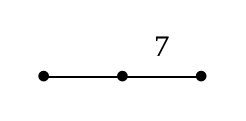
\begin{tikzpicture}
    \draw[thick] (0,0) node{$\bullet$} to (1,0) node{$\bullet$} to node[label=above:{7}]{} (2,0) node {$\bullet$};
  \end{tikzpicture}
\] we get a group having one generator for each dot, and with one
relation \(r^2 = 1\) for each generator \(r\) (since that's what
reflections do), and one relation of the form \((rs)^n = 1\) for each
line connecting dots, or \((rs)^2 = 1\) if there is no line connecting
two dots. It turns out that if a Coxeter diagram yields a \emph{finite}
group this way, it's a finite reflection group.

However, not every diagram we draw yields a finite group! Here are all
the possible Coxeter diagrams giving finite groups. They have names.
First there is \(A_n\), which has \(n\) dots like this: \[
  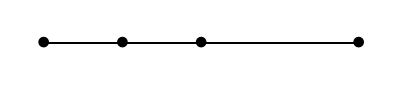
\begin{tikzpicture}
    \draw[thick] (0,0) node{$\bullet$} to (1,0) node{$\bullet$} to (2,0) node {$\bullet$} to (4,0) node{$\bullet$};
  \end{tikzpicture}
\] For example, the group of symmetries of the equilateral triangle is
\(A_2\). The two dots can correspond to the reflections \(r\) and \(s\)
through two of the altitudes of the triangle, which are at an angle of
\(\pi/3\) from each other. Thus they satisfy \((rs)^3 = 1\). More
generally, \(A_n\) corresponds to the group of symmetries of an
\(n\)-dimensional simplex --- which is just the group of permutations of
the \(n+1\) vertices.

Then there is \(B_n\), which has \(n\) dots, where \(n > 1\): \[
  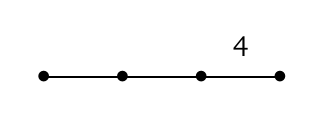
\begin{tikzpicture}
    \draw[thick] (0,0) node{$\bullet$} to (1,0) node{$\bullet$} to (2,0) node{$\bullet$} to node[label=above:{4}]{} (3,0) node {$\bullet$};
  \end{tikzpicture}
\] It has just one edge labelled with a 4. \(B_n\) turns out to be the
group of symmetries of a hypercube or hyperoctahedron in \(n\)
dimensions.

Then there is \(D_n\), where \(n > 3\): \[
  \begin{tikzpicture}
    \draw[thick] (0,0) node{$\bullet$} to (1,0) node{$\bullet$} to (2,0) node{$\bullet$} to (3,0) node {$\bullet$};
    \draw[thick] (3,0) to (4,1) node {$\bullet$};
    \draw[thick] (3,0) to (4,-1) node {$\bullet$};
  \end{tikzpicture}
\] Then there are \(E_6\), \(E_7\), and \(E_8\): \[
  \begin{gathered}
    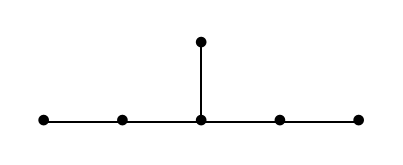
\begin{tikzpicture}
      \draw[thick] (0,0) node{$\bullet$} to (1,0) node{$\bullet$} to (2,0) node{$\bullet$} to (3,0) node {$\bullet$} to (4,0) node {$\bullet$};
      \draw[thick] (2,0) to (2,1) node{$\bullet$};
    \end{tikzpicture}
    \qquad
    \begin{tikzpicture}
      \draw[thick] (0,0) node{$\bullet$} to (1,0) node{$\bullet$} to (2,0) node{$\bullet$} to (3,0) node {$\bullet$} to (4,0) node {$\bullet$} to (5,0) node {$\bullet$};
      \draw[thick] (2,0) to (2,1) node{$\bullet$};
    \end{tikzpicture}
  \\\begin{tikzpicture}
      \draw[thick] (0,0) node{$\bullet$} to (1,0) node{$\bullet$} to (2,0) node{$\bullet$} to (3,0) node {$\bullet$} to (4,0) node {$\bullet$} to (5,0) node {$\bullet$} to (6,0) node {$\bullet$};
      \draw[thick] (2,0) to (2,1) node{$\bullet$};
    \end{tikzpicture}
  \end{gathered}
\] Interestingly, this series does \emph{not} go on. That's what I meant
about ``classical'' versus ``exceptional'' structures.

Then there is \(F_4\): \[
  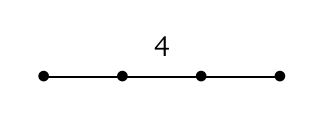
\begin{tikzpicture}
    \draw[thick] (0,0) node{$\bullet$} to (1,0) node{$\bullet$} to node[label=above:{4}]{} (2,0) node{$\bullet$} to (3,0) node {$\bullet$};
  \end{tikzpicture}
\] Then there's \(G_2\): \[
  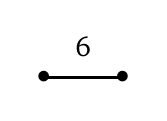
\begin{tikzpicture}
    \draw[thick] (0,0) node{$\bullet$} to node[label=above:{6}]{} (1,0) node{$\bullet$};
  \end{tikzpicture}
\] and \(H_3\) and \(H_4\): \[
  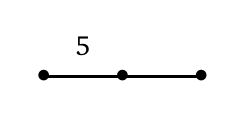
\begin{tikzpicture}
    \draw[thick] (0,0) node{$\bullet$} to node[label=above:{5}]{} (1,0) node{$\bullet$} to (2,0) node{$\bullet$};
  \end{tikzpicture}
  \qquad
  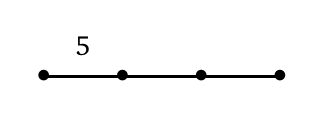
\begin{tikzpicture}
  \draw[thick] (0,0) node{$\bullet$} to node[label=above:{5}]{} (1,0) node{$\bullet$} to (2,0) node{$\bullet$} to (3,0) node {$\bullet$};
\end{tikzpicture}
\] \(H_3\) is the group of symmetries of the dodecahedron or
icosahedron. \(H_4\) is the group of symmetries of a regular solid in 4
dimensions which I talked about in \protect\hyperlink{week20}{``Week
20''}. This regular solid is also called the ``unit icosians'' --- it
has 120 vertices, and is a close relative of the icosahedron and
dodecahedron. One amazing thing is that it itself \emph{is} a group in a
very natural way. There are no ``hypericosahedra'' or
``hyperdodecahedra'' in dimensions greater than 4, which is related to
the fact that the \(H\) series quits at this point.

Finally, there is another infinite series, \(I_m\): \[
  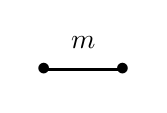
\begin{tikzpicture}
    \draw[thick] (0,0) node{$\bullet$} to node[label=above:{$m$}]{} (1,0) node{$\bullet$};
  \end{tikzpicture}
\] This corresponds to the symmetry group of the \(2m\)-gon in the
plane, and people usually require \(m = 5\) or \(m > 6\), so as to not
count twice some Coxeter diagrams that we've already run into.

THAT'S ALL.

So, we have an ``ABDEFGHI classification'' of finite reflection groups.
(In some future week I had better say what happened to ``C''.) Note that
the symmetry groups of the Platonic solids and some of their
higher-dimensional relatives fit in nicely into this classification, so
that's one sense in which the Greeks' discovery of these solids counts
as the first ``ADE classification''. But there is at least one another,
deeper, way to fit the Platonic solids themselves into an ADE
classification. I'll try to say more about this in future weeks.

You may still be wondering what's so special about A, D, and E. I'll
have to get to that, too.

\begin{center}\rule{0.5\linewidth}{0.5pt}\end{center}
\hypertarget{week63}{%
\section{September 14, 1995}\label{week63}}

Let me continue the tale of ``ADE classifications''. Last week I
described an ``ABDEFGHI classification'' of all finite reflection groups
- that is, finite symmetry groups of Euclidean space, every element of
which is a product of reflections. Now we'll build on that to get other
related classifications.

So, recall:

Every element of a finite reflection group is a product of reflections
through certain special vectors, which people call ``roots''. These
roots are all at angles \(\pi/n\) from each other, where \(n > 1\) is an
integer. To describe the group, we draw a diagram with one dot for each
root. If two roots are perpendicular we don't draw a line between them,
but otherwise, if they are at an angle \(\pi/n\) from each other, we
draw a line and label it with the integer \(n\). Actually, the integer
\(n = 3\) comes up so often that we don't bother labelling the line in
this case.

Now, not all of these diagrams correspond to finite reflection groups.
The following ones, together with disjoint unions of them, are all the
possibilities.

\begin{quote}
\(A_n\), which has \(n\) dots like this: \[
  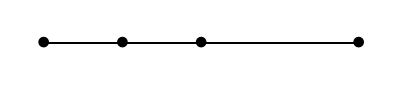
\begin{tikzpicture}
    \draw[thick] (0,0) node{$\bullet$} to (1,0) node{$\bullet$} to (2,0) node {$\bullet$} to (4,0) node{$\bullet$};
  \end{tikzpicture}
\] \(B_n\), which has \(n\) dots, where \(n > 1\): \[
  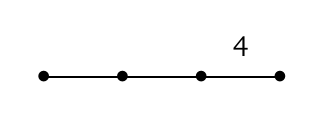
\begin{tikzpicture}
    \draw[thick] (0,0) node{$\bullet$} to (1,0) node{$\bullet$} to (2,0) node{$\bullet$} to node[label=above:{4}]{} (3,0) node {$\bullet$};
  \end{tikzpicture}
\] \(D_n\), which has \(n\) dots, where \(n > 3\): \[
  \begin{tikzpicture}
    \draw[thick] (0,0) node{$\bullet$} to (1,0) node{$\bullet$} to (2,0) node{$\bullet$} to (3,0) node {$\bullet$};
    \draw[thick] (3,0) to (4,1) node {$\bullet$};
    \draw[thick] (3,0) to (4,-1) node {$\bullet$};
  \end{tikzpicture}
\] \(E_6\), \(E_7\), and \(E_8\): \[
  \begin{gathered}
    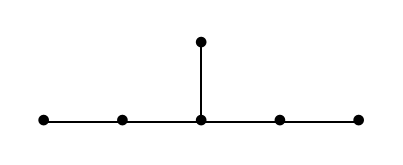
\begin{tikzpicture}
      \draw[thick] (0,0) node{$\bullet$} to (1,0) node{$\bullet$} to (2,0) node{$\bullet$} to (3,0) node {$\bullet$} to (4,0) node {$\bullet$};
      \draw[thick] (2,0) to (2,1) node{$\bullet$};
    \end{tikzpicture}
    \qquad
    \begin{tikzpicture}
      \draw[thick] (0,0) node{$\bullet$} to (1,0) node{$\bullet$} to (2,0) node{$\bullet$} to (3,0) node {$\bullet$} to (4,0) node {$\bullet$} to (5,0) node {$\bullet$};
      \draw[thick] (2,0) to (2,1) node{$\bullet$};
    \end{tikzpicture}
  \\\begin{tikzpicture}
      \draw[thick] (0,0) node{$\bullet$} to (1,0) node{$\bullet$} to (2,0) node{$\bullet$} to (3,0) node {$\bullet$} to (4,0) node {$\bullet$} to (5,0) node {$\bullet$} to (6,0) node {$\bullet$};
      \draw[thick] (2,0) to (2,1) node{$\bullet$};
    \end{tikzpicture}
  \end{gathered}
\] \(F_4\): \[
  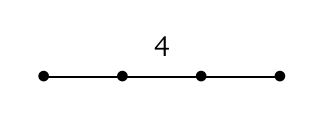
\begin{tikzpicture}
    \draw[thick] (0,0) node{$\bullet$} to (1,0) node{$\bullet$} to node[label=above:{4}]{} (2,0) node{$\bullet$} to (3,0) node {$\bullet$};
  \end{tikzpicture}
\] \(G_2\): \[
  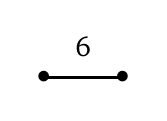
\begin{tikzpicture}
    \draw[thick] (0,0) node{$\bullet$} to node[label=above:{6}]{} (1,0) node{$\bullet$};
  \end{tikzpicture}
\] \(H_3\) and \(H_4\): \[
  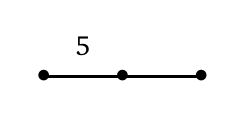
\begin{tikzpicture}
    \draw[thick] (0,0) node{$\bullet$} to node[label=above:{5}]{} (1,0) node{$\bullet$} to (2,0) node{$\bullet$};
  \end{tikzpicture}
  \qquad
  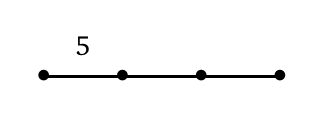
\begin{tikzpicture}
  \draw[thick] (0,0) node{$\bullet$} to node[label=above:{5}]{} (1,0) node{$\bullet$} to (2,0) node{$\bullet$} to (3,0) node {$\bullet$};
\end{tikzpicture}
\] \(I_m\), where \(m = 5\) or \(m > 6\): \[
  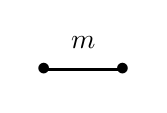
\begin{tikzpicture}
    \draw[thick] (0,0) node{$\bullet$} to node[label=above:{$m$}]{} (1,0) node{$\bullet$};
  \end{tikzpicture}
\]
\end{quote}

Recall that \(I_m\) is the symmetry group of the of regular \(m\)-gon,
while others of these are the symmetry groups of Platonic solids, and
still others are symmetry groups of regular polytopes in
\(n\)-dimensional space. For example, the symmetry group of the
dodecahedron is \(H_3\), while that of its 4-dimensional relative is
\(H_4\).

Now you may know that there are no perfect crystals in the shape of a
regular dodecahedron. However, iron pyrite comes close. In his wonderful
book:

\begin{enumerate}
\def\labelenumi{\arabic{enumi})}
\tightlist
\item
  Hermann Weyl, \emph{Symmetry}, Princeton University Press, Princeton,
  New Jersey, 1989.
\end{enumerate}

Weyl suggests that this is how people discovered the regular
dodecahedron:

\begin{quote}
\ldots the discovery of the last two {[}Platonic solids{]} is certainly
one of the most beautiful and singular discoveries made in the whole
history of mathematics. With a fair amount of certainty, it can be
traced to the colonial Greeks in southern Italy. The suggestion has been
made that they abstracted the regular dodecahedron from the crystals of
pyrite, a sulfurous mineral abundant in Sicily.
\end{quote}

Thus while iron pyrite is nothing but ``fool's gold'' to the miner, it
may have done a good deed by fooling the Greeks into discovering the
regular dodecahedron. Could this be why the ratio of the diagonal to the
side of a regular pentagon, \((\sqrt{5} + 1)/2\), is called the golden
ratio? Or am I just getting carried away? One is tempted to call the
shape of pyrite crystals the ``fool's dodecahedron,'' but in fact it's
called a ``pyritohedron''. (All this information on pyrite, as well as
the puns, I owe to Michael Weiss.)

More recently, I think people have discovered ``quasicrystals'' (related
to Penrose tiles) having true dodecahedral symmetry. But no perfectly
repetitive crystals form dodecahedra! And the reason is that there is no
lattice having \(H_3\) as its symmetries.

Recall that we get a ``lattice'' by taking \(n\) linearly independent
vectors in \(n\)-dimensional Euclidean space and forming all linear
combinations with integer coefficients. If someone hands us a finite
reflection group, we can look for a lattice having it as symmetries. If
one exists, we say the group satisfies the ``crystallographic
condition''. The only ones that do are

\[\mbox{$A_n$, $B_n$, $D_n$, $E_6$, $E_7$, $E_8$, $F_4$, and $G_2$}\]

(and those corresponding to disjoint unions of these diagrams). In other
words, the symmetry groups of the pentagon (\(I_5\)), the heptagon and
so on (\(I_m\) with \(m > 6\)), and the dodecahedron and its
4-dimensional relative (\(H_3\) and \(H_4\)) are ruled out.

Now let us turn to the theory of Lie groups. Lie groups are the most
important ``continuous'' (as opposed to discrete) symmetry groups.
Examples include the real line (with addition as the group operation),
the circle (with addition \(\mod 2\pi\)), and the groups \(SO(n)\) and
\(SU(n)\) discussed in \protect\hyperlink{week61}{``Week 61''}. These
groups are incredibly important in both physics and mathematics. Thus it
is wonderful, and charmingly ironic, that the same diagrams that
classify the oh-so-discrete finite reflection groups also classify some
of the most beautiful of Lie groups: the ``simple'' Lie groups. It turns
out that the simple Lie groups correspond to the diagrams of forms
\(A\),\(B\),\(D\),\(E\),\(F\), and \(G\). Oh yes, and \(C\). I have to
tell you what happened to \(C\).

There is a vast amount known about semisimple Lie groups, and everyone
really serious about mathematics winds up needing to learn some of this
stuff. I took courses on Lie groups and their Lie algebras in grad
school, but it was only later that I really came to appreciate the
beauty of the simple Lie groups. Back then I found it mystifying because
the work involved in the classification was so algebraic, and I
preferred the more geometrical aspects of Lie groups. Part of the reason
is that the treatment I learned emphasized the Lie algebras and
downplayed the groups. A nice treatment that emphasizes the groups is:

\begin{enumerate}
\def\labelenumi{\arabic{enumi})}
\setcounter{enumi}{1}
\tightlist
\item
  John Frank Adams, \emph{Lectures on Lie groups}, Benjamin, New York,
  1969.
\end{enumerate}

So what's the basic idea? Let me summarize two semesters of grad school,
and tell you the basic stuff about Lie groups and the classification of
simple Lie groups. Forgive me if it's a bit rushed, sketchy, and even
mildly inaccurate: hopefully the main ideas will shine through the murk
this way.

A Lie group is a group that's also a manifold, for which the group
operations (multiplication and taking inverses) are smooth functions.
This lets you form the tangent space to any point in the group, and the
tangent space at the identity plays a special role. It's called the Lie
algebra of the group. If we have any element \(x\) in the Lie algebra,
we can exponentiate it to get an element \(\exp(x)\) in the group, and
we can keep track of the noncommutativity of the group by forming the
``bracket'' of elements \(x\) and \(y\) in the Lie algebra:

\[[x,y] = \frac{d}{dt}\frac{d}{ds} \exp(sx) \exp(ty) \exp(-sx) \exp(-ty)\]

where \(s\) and \(t\) are real numbers, and we evaluate the derivative
at \(s,t = 0\). Note that \([x,y] = 0\) if the group is commutative.
This bracket operation satisfies some axioms, and algebraists call
anything a Lie algebra that satisfies those axioms. For example, you
could take \(n \times n\) matrices and let \([x,y] = xy - yx\).

Now a Lie algebra is called ``semisimple'' if for any \(z\), there are
\(x\) and \(y\) with \(z = [x,y]\). This is sort of the opposite of an
abelian, or commutative, Lie algebra, where \([x,y] = 0\) for all \(x\)
and \(y\). It turns out that we can take direct sums of Lie algebras by
defining operations componentwise, and it turns out that if you have a
\emph{compact} Lie group, its Lie algebra is always the direct sum of a
semsimple Lie algebra and an abelian one. The abelian ones are pretty
trivial, so all the hard works lies in understanding the semisimple
ones. Any semisimple one is the direct sum of a bunch of semisimple ones
that aren't sums of anything else, and these basic building blocks are
called the ``simple'' ones. They are like the prime numbers of Lie
algebra theory. Unlike the prime numbers, though, we can completely
classify all of them!

Now how does one classify the simple Lie algebras? Basically, it goes
like this. We'll assume our simple Lie algebra is the Lie algebra of a
compact Lie group \(G\) --- it turns out that they all are. Now, sitting
inside \(G\) there is a maximal commutative subgroup \(T\) that's a
torus: a product of a bunch of circles. Let \(\mathrm{Lie}(T)\) stand
for the Lie algebra of this torus \(T\). Now, sitting inside
\(\mathrm{Lie}(T)\) there is a lattice, consisting of all elements \(x\)
with \(\exp(x) = 1\). This is how lattices sneak into the picture!

Moreover, for some elements \(g\) in \(G\), if we ``conjugate'' \(T\) by
\(g\), that is, form the set of all elements \(gtg^{-1}\) where \(t\) is
in \(T\), we get \(T\) back. In other words, these elements of \(g\) act
as symmetries of the torus \(T\). Now, if something acts as symmetries
of something else, it also acts as symmetries of everything naturally
cooked up from that something else. (Roughly speaking, ``naturally''
means "without dependence on arbitrary choices.) For this reason, these
special elements of \(G\) also act as symmetries of \(\mathrm{Lie}(T)\)
and of the lattice sitting inside \(\mathrm{Lie}(T)\). So we have a
lattice together with a group of symmetries, which by the way is called
the Weyl group of \(G\). Now the cool part is that the Weyl group is
actually a finite reflection group, so it must correspond to one of the
diagrams in the list above! Even better, it turns out that the Lie
algebra of \(G\) is determined by the lattice together with its Weyl
group.

The upshot is that to classify semisimple Lie algebras, all we need is
the classification of finite reflection groups satisfying the
crystallographic condition --- which we've done already using diagrams
--- together with a classification of lattices having such finite
reflection groups as symmetries. It turns out that the operation of
taking direct sums of semisimple Lie algebras corresponds to taking
disjoint unions of diagrams, so to get the ``building blocks'' --- the
\emph{simple} Lie algebras --- we only need to worry about the diagrams
we've drawn above, not disjoint unions of them. Now it turns out that
for every type except \(B\), there is (up to isomorphism) only
\emph{one} lattice having that group of symmetries, but for \(B\) there
are two. Recall the diagram \(B_n\) looks like: \[
  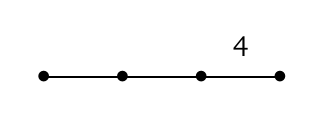
\begin{tikzpicture}
    \draw[thick] (0,0) node{$\bullet$} to (1,0) node{$\bullet$} to (2,0) node{$\bullet$} to node[label=above:{4}]{} (3,0) node {$\bullet$};
  \end{tikzpicture}
\] with \(n\) dots. And recall that the dots correspond to ``roots'',
which in the present context are vectors in \(\mathrm{Lie}(T)\). Now it
turns out that whenever we have a finite reflection group satisfying the
crystallographic condition, we can get a lattice having it as symmetries
by taking integer linear combinations of the roots, but \emph{not}
necessarily roots that are unit vectors; the lengths of the roots
matter. In all cases except \(B\), there is basically just one way to
get the lengths right, but for \(B\) there are two. We can keep track of
the root lengths with some extra markings on our diagrams, and then we
get two diagrams, which we call \(B_n\) and \(C_n\). One of them has the
root at the right of the diagram being longer, and one has the root
right next to it being longer. This makes no difference when \(n = 2\),
since then we just have \[
  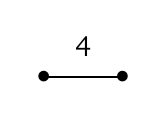
\begin{tikzpicture}
    \draw[thick] (0,0) node{$\bullet$} to node[label=above:{4}]{} (1,0) node {$\bullet$};
  \end{tikzpicture}
\] which is perfectly symmetrical. So folks usually consider \(C_n\)
only for \(n > 2\), to avoid double counting.

In other words, all the simple Lie algebras are of the form:

\begin{itemize}
\tightlist
\item
  \(A_n\), \(n > 0\)
\item
  \(B_n\), \(n > 1\)
\item
  \(C_n\), \(n > 2\)
\item
  \(D_n\), \(n > 3\)
\item
  \(E_6\), \(E_7\), \(E_8\)
\item
  \(F_4\)
\item
  \(G_2\)
\end{itemize}

Okay, so what \emph{are} these things, really? What do they \emph{mean},
and what are the implications of the fact that the symmetries of the
forces of nature are given by the some of the corresponding Lie groups?
Why are 4 infinite series of them and 5 ``exceptional'' Lie algebras?
What's so special about A, D, and E, that makes people keep talking
about ``ADE classifications''? What do the exceptional Lie algebras (and
their corresponding Lie groups) have to do with octonions? Why do some
string theorists think the symmetry group of nature is \(E_8\), the
largest exceptional Lie group???

Well, I'm afraid that I'm going camping in a couple of hours, so I'll
have to leave you hanging, even though I do know the answers to
\emph{some} of these questions. I'll try to finish talking about ADE
classifications in the next couple of issues.

\begin{center}\rule{0.5\linewidth}{0.5pt}\end{center}

\emph{\ldots{} without fantasy one would never become a mathematician,
and what gave me a place among the mathematicians of our day, despite my
lack of knowledge and form, was the audacity of my thinking.} - Sophus
Lie
\hypertarget{week64}{%
\section{September 23, 1995}\label{week64}}

I have been talking about different ``ADE classifications''. This time
I'll start by continuing the theme of last Week, namely simple Lie
algebras, and then move on to discuss affine Lie algebras and quantum
groups. These are algebraic structures that describe the symmetries
appearing in quantum field theory in 2 and 3 dimensions. They are very
important in string theory and topological quantum field theory, and
it's largely physics that has gotten people interested in them.

Remember, we began by classifying finite reflection groups. A finite
reflection group is simply a finite group of linear transformations of
\(\mathbb{R}^n\), every element of which is a product of reflections.
Finite reflection groups are in 1-1 correspondence with the following
``Coxeter diagrams'', together with disjoint unions of such diagrams:

\begin{quote}
\(A_n\), which has \(n\) dots like this: \[
  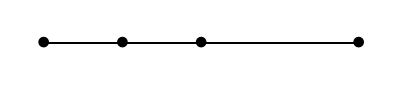
\begin{tikzpicture}
    \draw[thick] (0,0) node{$\bullet$} to (1,0) node{$\bullet$} to (2,0) node {$\bullet$} to (4,0) node{$\bullet$};
  \end{tikzpicture}
\] \(B_n\), which has \(n\) dots, where \(n > 1\): \[
  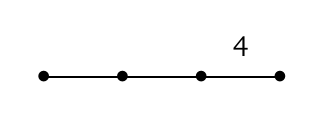
\begin{tikzpicture}
    \draw[thick] (0,0) node{$\bullet$} to (1,0) node{$\bullet$} to (2,0) node{$\bullet$} to node[label=above:{4}]{} (3,0) node {$\bullet$};
  \end{tikzpicture}
\] \(D_n\), which has \(n\) dots, where \(n > 3\): \[
  \begin{tikzpicture}
    \draw[thick] (0,0) node{$\bullet$} to (1,0) node{$\bullet$} to (2,0) node{$\bullet$} to (3,0) node {$\bullet$};
    \draw[thick] (3,0) to (4,1) node {$\bullet$};
    \draw[thick] (3,0) to (4,-1) node {$\bullet$};
  \end{tikzpicture}
\] \(E_6\), \(E_7\), and \(E_8\): \[
  \begin{gathered}
    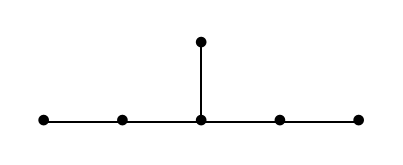
\begin{tikzpicture}
      \draw[thick] (0,0) node{$\bullet$} to (1,0) node{$\bullet$} to (2,0) node{$\bullet$} to (3,0) node {$\bullet$} to (4,0) node {$\bullet$};
      \draw[thick] (2,0) to (2,1) node{$\bullet$};
    \end{tikzpicture}
    \qquad
    \begin{tikzpicture}
      \draw[thick] (0,0) node{$\bullet$} to (1,0) node{$\bullet$} to (2,0) node{$\bullet$} to (3,0) node {$\bullet$} to (4,0) node {$\bullet$} to (5,0) node {$\bullet$};
      \draw[thick] (2,0) to (2,1) node{$\bullet$};
    \end{tikzpicture}
  \\\begin{tikzpicture}
      \draw[thick] (0,0) node{$\bullet$} to (1,0) node{$\bullet$} to (2,0) node{$\bullet$} to (3,0) node {$\bullet$} to (4,0) node {$\bullet$} to (5,0) node {$\bullet$} to (6,0) node {$\bullet$};
      \draw[thick] (2,0) to (2,1) node{$\bullet$};
    \end{tikzpicture}
  \end{gathered}
\] \(F_4\): \[
  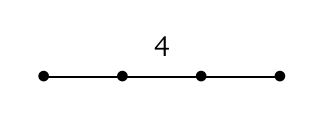
\begin{tikzpicture}
    \draw[thick] (0,0) node{$\bullet$} to (1,0) node{$\bullet$} to node[label=above:{4}]{} (2,0) node{$\bullet$} to (3,0) node {$\bullet$};
  \end{tikzpicture}
\] \(G_2\): \[
  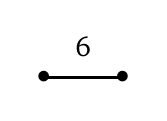
\begin{tikzpicture}
    \draw[thick] (0,0) node{$\bullet$} to node[label=above:{6}]{} (1,0) node{$\bullet$};
  \end{tikzpicture}
\] \(H_3\) and \(H_4\): \[
  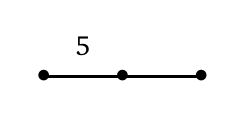
\begin{tikzpicture}
    \draw[thick] (0,0) node{$\bullet$} to node[label=above:{5}]{} (1,0) node{$\bullet$} to (2,0) node{$\bullet$};
  \end{tikzpicture}
  \qquad
  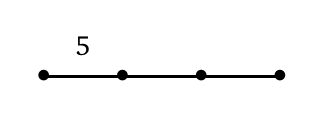
\begin{tikzpicture}
  \draw[thick] (0,0) node{$\bullet$} to node[label=above:{5}]{} (1,0) node{$\bullet$} to (2,0) node{$\bullet$} to (3,0) node {$\bullet$};
\end{tikzpicture}
\] \(I_m\), where \(m = 5\) or \(m > 6\): \[
  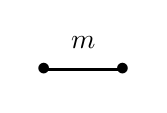
\begin{tikzpicture}
    \draw[thick] (0,0) node{$\bullet$} to node[label=above:{$m$}]{} (1,0) node{$\bullet$};
  \end{tikzpicture}
\]
\end{quote}

Not all of these finite reflection groups satisfy the ``crystallographic
condition'', namely that they act as symmetries of some lattice. The
ones that do are of types A,B,D,E,F, and G, and disjoint unions thereof
--- but I'm going to stop reminding you about disjoint unions all the
time!

Now, if we have a finite reflection group that's the symmetries of some
lattice, we can take the dimension of the lattice to be the number of
dots in the Coxeter diagram. In fact, the dots correspond to a basis of
the lattice, and the lines between them (and their numberings) keep
track of the angles between the basis vectors. These basis vectors are
called ``roots''. To describe the lattice completely, in principle we
need to know the lengths of the roots as well as the angles between
them. But it turns out that except for type B, there is just one choice
of lengths that works (up to overall scale). For type B there are two
choices, which people call \(B_n\) and \(C_n\), respectively. People
keep track of the lengths with a ``Dynkin diagram'' like this:

\begin{itemize}
\tightlist
\item
  \(B_n\) has \(n\) dots, where \(n>1\): \[
      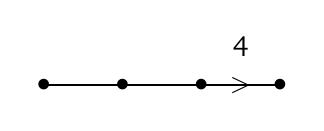
\begin{tikzpicture}
        \draw[thick] (0,0) node{$\bullet$} to (1,0) node{$\bullet$} to (2,0) node{$\bullet$} to node[label=above:{4}]{\textgreater} (3,0) node {$\bullet$};
      \end{tikzpicture}
    \]
\item
  \(C_n\) has \(n\) dots, where \(n>2\): \[
      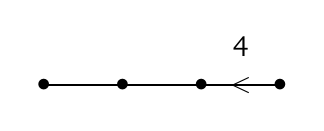
\begin{tikzpicture}
        \draw[thick] (0,0) node{$\bullet$} to (1,0) node{$\bullet$} to (2,0) node{$\bullet$} to node[label=above:{4}]{\textless} (3,0) node {$\bullet$};
      \end{tikzpicture}
    \]
\end{itemize}

The arrow points to the shorter root; for \(B_n\) all the roots except
the last one are \(\sqrt{2}\) times as long as the last one, while for
\(C_n\) all the roots except the last one are \(1/\sqrt{2}\) as long.
(In fact, the lattices corresponding to \(B_n\) and \(C_n\) are
``dual'', in the hopefully obvious sense.) The only reason why we
require \(n > 2\) for \(C_n\) is that \(B_2\) is basically the same as
\(C_2\)!

Now last Week, I also sketched how the Lie algebras of the compact
simple Lie groups were \emph{also} classified by the same Dynkin
diagrams of types A, B, C, D, E, F, and G. These were real Lie algebras;
we can also switch viewpoint and work with complex Lie algebras if we
like, in which case we simply say we're studying the complex simple Lie
algebras, as opposed to their ``compact real forms''.

Unfortunately, I didn't say much about what these Lie algebras actually
are! Basically, they go like this:

\(A_n\) --- The Lie algebra \(A_n\) is just
\(\mathfrak{sl}_{n+1}(\mathbb{C})\), the \((n+1) \times (n+1)\) complex
matrices with vanishing trace, which form a Lie algebra with the usual
bracket \([x,y] = xy -yx\). The compact real form of
\(\mathfrak{sl}_n(\mathbb{C})\) is \(\mathfrak{su}_n\), and the
corresponding compact Lie group is \(SU(n)\), the \(n\times n\) unitary
matrices with determinant \(1\). The symmetry group of the electroweak
force is \(U(1) \times SU(2)\), where \(U(1)\) is the \(1 \times 1\)
unitary matrices. The symmetry group of the strong force is \(SU(3)\).
The study of \(A_n\) is thus a big deal in particle physics. People have
also considered ``grand unified theories'' with symmetry groups like
\(SU(5)\).

\(B_n\) --- The Lie algebra \(B_n\) is
\(\mathfrak{so}_{2n+1}(\mathbb{C})\), the \((2n+1) \times (2n+1)\)
skew-symmetric complex matrices with vanishing trace. The compact real
form of \(\mathfrak{so}_n(\mathbb{C})\) is \(\mathfrak{so}_n\), and the
corresponding compact Lie group is \(SO(n)\), the \(n \times n\) real
orthogonal matrices with determinant \(1\), that is, the rotation group
in Euclidean \(n\)-space. For some basic cool facts about \(SO(n)\),
check out \protect\hyperlink{week61}{``Week 61''}.

\(C_n\) --- The Lie algebra \(C_n\) is \(\mathfrak{sp}_n(\mathbb{C})\),
the \(2n \times 2n\) complex matrices of the form \[
  \left(
    \begin{array}{cc}
      A&B\\C&D
    \end{array}
  \right)
\] where \(B\) and \(C\) are symmetric, and \(D\) is minus the transpose
of \(A\). The compact real form of \(\mathfrak{sp}_n(\mathbb{C})\) is
\(\mathfrak{sp}_n\), and the corresponding compact Lie group is called
\(Sp(n)\). This is the group of \(n \times n\) quaternionic matrices
which preserve the usual inner product on the space \(\mathbb{H}^n\) of
\(n\)-tuples of quaternions.

\(D_n\) --- The Lie algebra \(D_n\) is
\(\mathfrak{so}_{2n}(\mathbb{C})\), the \(2n \times 2n\) skew-symmetric
complex matrices with vanishing trace. See \(B_n\) above for more about
this. It may seem weird that \(SO(n)\) acts so differently depending on
whether \(n\) is even or odd, but it's true: for example, there are
``left-handed'' and ``right-handed'' spinors in even dimensions, but not
in odd dimensions. Some clues as to why are given in
\protect\hyperlink{week61}{``Week 61''}.

Those are the ``classical'' Lie algebras, and they are things that are
pretty easy to reinvent for yourself, and to get interested in for all
sorts of reasons. As you can see, they are all about ``rotations'' in
real, complex, and quaternionic vector spaces.

The remaining ones are called ``exceptional'', and they are much more
mysterious. They were only discovered when people figured out the
classification of simple Lie algebras. As it turns out, they tend to be
related to the octonions! Some other week I will say more about them,
but for now, let me just say:

\(F_4\) --- This is a 52-dimensional Lie algebra. Its smallest
representation is 26-dimensional, consisting of the traceless
\(3\times3\) hermitian matrices over the octonions, on which it
preserves a trilinear form.

\(G_2\) --- This is a 14-dimensional Lie algebra, and the compact Lie
group corresponding to its compact real form is also often called
\(G_2\). This group is just the group of symmetries (automorphisms) of
the octonions! In fact, the smallest representation of this Lie algebra
is 7-dimensional, corresponding to the purely imaginary octonions.

\(E_6\) --- This is a 78-dimensional Lie algebra. Its smallest
representation is 27-dimensional, consisting of all the \(3\times3\)
hermitian matrices over the octonions this time, on which it preserves
the anticommutator.

\(E_7\) --- This is a 133-dimensional Lie algebra. Its smallest
representation is 56-dimensional, on which it preserves a tetralinear
form.

\(E_8\) --- This is a 248-dimensional Lie algebra, the biggest of the
exceptional Lie algebras. Its smallest representation is
248-dimensional, the so-called ``adjoint'' representation, in which it
acts on itself. Thus in some vague sense, the simplest way to understand
the Lie group corresponding to \(E_8\) is as the symmetries of itself!
(Thanks go to Dick Gross for this charming information; I think he said
all the other exceptional Lie algebras have representations smaller than
themselves, but I forget the sizes.) In
\protect\hyperlink{week20}{``Week 20''} I described a way to get its
root lattice (the 8-dimensional lattice spanned by the roots) by playing
around with the icosahedron and the quaternions.

People have studied simple Lie algebras a lot this century, basically
studied the hell out of them, and in fact some people were getting a
teeny bit sick of it recently, when along came some new physics that put
a lot of new life into the subject. A lot of this new physics is related
to string theory and quantum gravity. Some of this physics is
``conformal field theory'', the study of quantum fields in 2 dimensional
spacetime that are invariant under all conformal (angle-preserving)
transformations. This is important in string theory because the string
worldsheet is 2-dimensional. Some other hunks of this physics go by the
name of ``topological quantum field theory'', which is the study of
quantum fields, usually in 3 dimensions so far, that are invariant under
\emph{all} transformations (or more precisely, all diffeomorphisms).

Every simple Lie algebra gives rise to an ``affine Lie algebra'' and a
``quantum group''. The symmetries of conformal field theories are
closely related to affine Lie algebras, and the symmetries of
topological quantum field theories are quantum groups. I won't tell you
what affine Lie algebras and quantum groups ARE, since it would take
quite a while. Instead I'll refer you to a good good introduction to
this stuff:

\begin{enumerate}
\def\labelenumi{\arabic{enumi})}
\tightlist
\item
  Juergen Fuchs, \emph{Affine Lie Algebras and Quantum Groups},
  Cambridge Monographs on Mathematical Physics, Cambridge U. Press,
  Cambridge 1992.
\end{enumerate}

Let me whiz through his table of contents and very roughly sketch what
it's all about.

\begin{enumerate}
\def\labelenumi{\arabic{enumi}.}
\item
  \textbf{Semisimple Lie algebras}

  This is a nice summary of the theory of semisimple Lie algebras
  (remember, those are just direct sums of simple Lie algebras) and
  their representations. Especially if you are a physicist, a slick
  summary like this might be a better way to start learning the subject
  than a big fat textbook on the subject. He covers the Dynkin diagram
  stuff and much, much more.
\item
  \textbf{Affine Lie algebras}

  This starts by describing Kac-Moody algebras, which are certain
  \emph{infinite-dimensional} analogs of the simple Lie algebras. Fuchs
  concentrates on a special class of these, the affine Lie algebras, and
  describes the classification of these using Dynkin diagrams. The main
  nice thing about the affine Lie algebras is that their corresponding
  infinite-dimensional Lie groups are very nice: they are almost ``loop
  groups''. If we have a Lie group \(G\), the loop group \(LG\) is just
  the set of all smooth functions from the circle to \(G\), which we
  make into a group by pointwise multiplication. If you're a physicist,
  this is obviously relevant to string theory, because at each time, a
  string is just a circle (or bunch of circles), and if you are doing
  gauge theory on the string, with symmetry group \(G\), the gauge group
  is then just the loop group \(LG\). So you'd expect the representation
  theory of loop groups and their Lie algebras to be really important.

  You'd \emph{almost} be right, but there is a slight catch. In quantum
  theory, what counts are the ``projective'' representations of a group,
  that is, representations that satisfy the rule \(g(h(v)) = (gh)(v)\)
  \emph{up to a phase}. (This is because ``phases are unobservable in
  quantum theory'' --- one of those mottoes that needs to be carefully
  interpreted to be correct.) The projective representations of the loop
  group \(LG\) correspond to the honest-to-goodness representations of a
  ``central extensions'' of \(LG\), a slightly fancier group than \(LG\)
  itself. And the Lie algebra of \emph{this} group is called an affine
  Lie algebra.

  So, people who like gauge theory and string theory need to know a lot
  about affine Lie algebras and their representations, and that's what
  this chapter covers. A real heavy-duty string theorist will need to
  know more about Kac-Moody algebras, so if you're planning on becoming
  one of those, you'd better also try:

  \begin{enumerate}
  \def\labelenumii{\arabic{enumii})}
  \setcounter{enumii}{1}
  \tightlist
  \item
    Victor Kac, \emph{Infinite Dimensional Lie Algebras}, 3rd ed.,
    Cambridge University Press, Cambridge, 1990.
  \end{enumerate}

  You'll also need to know more about loop groups, so try:

  \begin{enumerate}
  \def\labelenumii{\arabic{enumii})}
  \setcounter{enumii}{2}
  \tightlist
  \item
    \emph{Loop groups}, by Andrew Pressley and Graeme Segal, Oxford
    University Press, Oxford, 1986.
  \end{enumerate}
\item
  \textbf{WZW theories}

  Well, I just said that physicists liked affine Lie algebras because
  they were the symmetries of conformal field theories that were also
  gauge theories. Guess what: a Wess-Zumino-Witten, or WZW, theory, is a
  conformal field theory that's also a gauge theory! You can think of it
  as the natural generalization of the wave equation in 2 dimension
  (which is conformally invariant, btw) from the case of real-valued
  fields, to general \(G\)-valued fields, where \(G\) is our favorite
  Lie group.
\item
  \textbf{Quantum groups}

  When you quantize a WZW theory whose symmetry group \(G\) is some
  simple Lie group, something funny happens. In a sense, the group
  itself also gets quantized! In other words, the algebraic structure of
  the group, or its Lie algebra, gets ``deformed'' in a way that depends
  on the parameter \(\hbar\) (Planck's constant). I have muttered much
  about quantum groups on This Week's Finds, especially concerning their
  relevance to topological quantum field theory, and I will not try to
  explain them any better here! Eventually I will discuss a bunch of
  books that have come out on quantum groups, and I hope to give a
  mini-introduction to the subject in the process.
\item
  \textbf{Duality, fusion rules, and modular invariance}

  The previous chapter described quantum groups as abstract algebraic
  structures, showing how you can get one from any simple Lie algebra.
  Here Fuchs really shows how you get them from quantizing a WZW theory.
  WZW theories are invariant under conformal transformations, and
  quantum groups inherit lots of cool properties from this fact. For
  example, suppose you form a torus by taking the complex plane and
  identifying two points if they differ by any number of the form
  \(n z_1 + m z_2\), where \(z_1\) and \(z_2\) are fixed complex numbers
  and \(n\), \(m\) are arbitrary integers. For example, we might
  identify all these points: \[
     \begin{tikzpicture}[scale=0.7]
       \draw[->] (-2,0) to (4,0) node[label=below:{$\Re(z)$}]{};
       \draw[->] (0,-3) to (0,4) node[label=left:{$\Im(z)$}]{};
       \foreach \m in {-1,0,1,2}
       {
         \foreach \n in {-1,0,1,2}
         {
           \node at ({\m*1.5-\n/3-0.2},{1.5*\n+\m-0.5}) {$\bullet$};
         }
       }
     \end{tikzpicture}
   \] The resulting torus is a ``Riemann surface'' and it has lots of
  transformations, called ``modular transformations''. The group of
  modular transformations is the discrete group \(SL(2,\mathbb{Z})\) of
  \(2\times2\) integer matrices with determinant \(1\); I leave it as an
  easy exercise to guess how these give transformations of the torus.
  (This is an example of a ``mapping class group'' as discussed in
  \protect\hyperlink{week28}{``Week 28''}.) In any event, the way the
  the WZW theory transforms under modular transformations translates
  into some cool properties of the corresponding quantum group, which
  Fuchs discusses. That's roughly what ``modular invariance'' means.

  Similarly, ``fusion rules'' have to do with the thrice-punctured
  sphere, or ``trinion'', which is another Riemann surface. And
  ``duality'' has to do with the sphere with four punctures, which can
  be viewed as built up from trinions in either of two ``dual'' ways: \[
     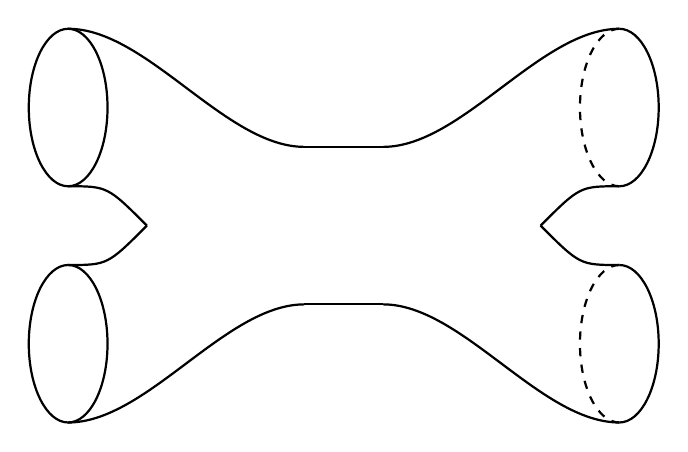
\begin{tikzpicture}[scale=0.5,rotate=90]
       \begin{scope}
         \draw[thick] (-3,0) ellipse (2cm and 1cm);
         \draw[thick] (3,0) ellipse (2cm and 1cm);
         \draw[thick] (-5,0) .. controls (-5,-2) and (-2,-4) .. (-2,-6);
         \draw[thick] (5,0) .. controls (5,-2) and (2,-4) .. (2,-6);
         \draw[thick] (-1,0) .. controls (-1,-1) .. (0,-2);
         \draw[thick] (1,0) .. controls (1,-1) .. (0,-2);
         \draw[thick] (-2,-6) to (-2,-7);
         \draw[thick] (2,-6) to (2,-7);
       \end{scope}
       \begin{scope}[rotate=180,shift={(0,14)}]
         \begin{scope}[shift={(-3,0)},rotate=180]
           \draw[thick,dashed] (0:2cm and 1cm) arc (0:180:2cm and 1cm);
           \draw[thick] (180:2cm and 1cm) arc (180:360:2cm and 1cm);
         \end{scope}
         \begin{scope}[shift={(3,0)},rotate=180]
           \draw[thick,dashed] (0:2cm and 1cm) arc (0:180:2cm and 1cm);
           \draw[thick] (180:2cm and 1cm) arc (180:360:2cm and 1cm);
         \end{scope}
         \draw[thick] (-5,0) .. controls (-5,-2) and (-2,-4) .. (-2,-6);
         \draw[thick] (5,0) .. controls (5,-2) and (2,-4) .. (2,-6);
         \draw[thick] (-1,0) .. controls (-1,-1) .. (0,-2);
         \draw[thick] (1,0) .. controls (1,-1) .. (0,-2);
         \draw[thick] (-2,-6) to (-2,-7);
         \draw[thick] (2,-6) to (2,-7);
       \end{scope}
     \end{tikzpicture}
   \] or \[
     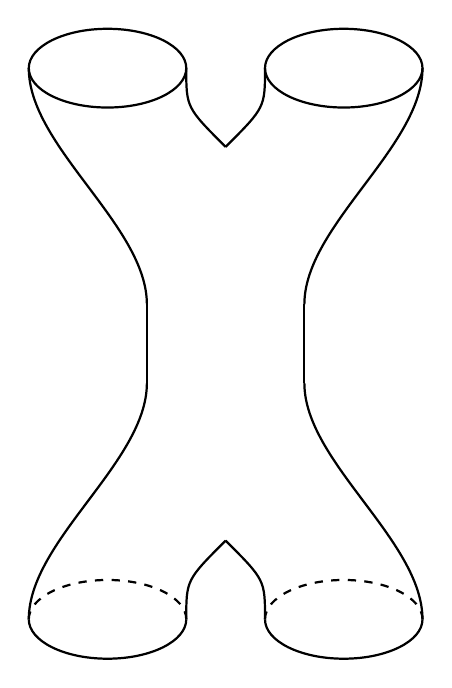
\begin{tikzpicture}[scale=0.5]
       \begin{scope}
         \draw[thick] (-3,0) ellipse (2cm and 1cm);
         \draw[thick] (3,0) ellipse (2cm and 1cm);
         \draw[thick] (-5,0) .. controls (-5,-2) and (-2,-4) .. (-2,-6);
         \draw[thick] (5,0) .. controls (5,-2) and (2,-4) .. (2,-6);
         \draw[thick] (-1,0) .. controls (-1,-1) .. (0,-2);
         \draw[thick] (1,0) .. controls (1,-1) .. (0,-2);
         \draw[thick] (-2,-6) to (-2,-7);
         \draw[thick] (2,-6) to (2,-7);
       \end{scope}
       \begin{scope}[rotate=180,shift={(0,14)}]
         \begin{scope}[shift={(-3,0)},rotate=180]
           \draw[thick,dashed] (0:2cm and 1cm) arc (0:180:2cm and 1cm);
           \draw[thick] (180:2cm and 1cm) arc (180:360:2cm and 1cm);
         \end{scope}
         \begin{scope}[shift={(3,0)},rotate=180]
           \draw[thick,dashed] (0:2cm and 1cm) arc (0:180:2cm and 1cm);
           \draw[thick] (180:2cm and 1cm) arc (180:360:2cm and 1cm);
         \end{scope}
         \draw[thick] (-5,0) .. controls (-5,-2) and (-2,-4) .. (-2,-6);
         \draw[thick] (5,0) .. controls (5,-2) and (2,-4) .. (2,-6);
         \draw[thick] (-1,0) .. controls (-1,-1) .. (0,-2);
         \draw[thick] (1,0) .. controls (1,-1) .. (0,-2);
         \draw[thick] (-2,-6) to (-2,-7);
         \draw[thick] (2,-6) to (2,-7);
       \end{scope}
     \end{tikzpicture}
   \] This is one of the reasons string theory was first discovered ---
  we can think of the above pictures as two Feynman diagrams for
  interacting strings, and the fact that they are really just distorted
  versions of each other gives rise to identities among Feynman
  diagrams. Similarly, this fact gives rise to identities satisfied by
  the fusion rules of quantum groups.
\end{enumerate}

So --- Fuchs' book should make clear how, starting from the austere
beauty of the Dynkin diagrams, we get not only simple Lie groups, but
also a wealth of more complicated structures that people find important
in modern theoretical physics.

\begin{center}\rule{0.5\linewidth}{0.5pt}\end{center}

\emph{Mathematics, rightly viewed, possesses not only truth, but supreme
beauty - a beauty cold and austere, like that of sculpture, without
appeal to any part of our weaker nature, without the gorgeous trappings
of painting or music, yet sublimely pure, and capable of a stern
perfection such as only the greatest art can show.} - Bertrand Russell.
\hypertarget{week65}{%
\section{October 3, 1995}\label{week65}}

This time I'll finish up talking about ``ADE classifications'' for a
while, although there is certainly more to say. Recall where we were:
the following diagrams correspond to the simple Lie algebras, and they
also define certain lattices, the ``root lattices'' of those Lie
algebras:

\begin{quote}
\(A_n\), which has \(n\) dots like this: \[
  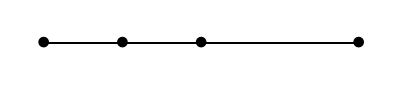
\begin{tikzpicture}
    \draw[thick] (0,0) node{$\bullet$} to (1,0) node{$\bullet$} to (2,0) node {$\bullet$} to (4,0) node{$\bullet$};
  \end{tikzpicture}
\] \(B_n\), which has \(n\) dots, where \(n > 1\): \[
  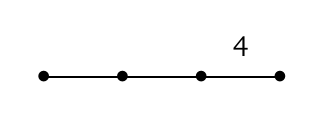
\begin{tikzpicture}
    \draw[thick] (0,0) node{$\bullet$} to (1,0) node{$\bullet$} to (2,0) node{$\bullet$} to node[label=above:{4}]{} (3,0) node {$\bullet$};
  \end{tikzpicture}
\] \(D_n\), which has \(n\) dots, where \(n > 3\): \[
  \begin{tikzpicture}
    \draw[thick] (0,0) node{$\bullet$} to (1,0) node{$\bullet$} to (2,0) node{$\bullet$} to (3,0) node {$\bullet$};
    \draw[thick] (3,0) to (4,1) node {$\bullet$};
    \draw[thick] (3,0) to (4,-1) node {$\bullet$};
  \end{tikzpicture}
\] \(E_6\), \(E_7\), and \(E_8\): \[
  \begin{gathered}
    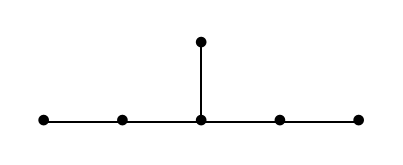
\begin{tikzpicture}
      \draw[thick] (0,0) node{$\bullet$} to (1,0) node{$\bullet$} to (2,0) node{$\bullet$} to (3,0) node {$\bullet$} to (4,0) node {$\bullet$};
      \draw[thick] (2,0) to (2,1) node{$\bullet$};
    \end{tikzpicture}
    \qquad
    \begin{tikzpicture}
      \draw[thick] (0,0) node{$\bullet$} to (1,0) node{$\bullet$} to (2,0) node{$\bullet$} to (3,0) node {$\bullet$} to (4,0) node {$\bullet$} to (5,0) node {$\bullet$};
      \draw[thick] (2,0) to (2,1) node{$\bullet$};
    \end{tikzpicture}
  \\\begin{tikzpicture}
      \draw[thick] (0,0) node{$\bullet$} to (1,0) node{$\bullet$} to (2,0) node{$\bullet$} to (3,0) node {$\bullet$} to (4,0) node {$\bullet$} to (5,0) node {$\bullet$} to (6,0) node {$\bullet$};
      \draw[thick] (2,0) to (2,1) node{$\bullet$};
    \end{tikzpicture}
  \end{gathered}
\] \(F_4\): \[
  \begin{tikzpicture}
    \draw[thick] (0,0) node{$\bullet$} to (1,0) node{$\bullet$} to node[label=above:{4}]{} (2,0) node{$\bullet$} to (3,0) node {$\bullet$};
  \end{tikzpicture}
\] \(G_2\): \[
  \begin{tikzpicture}
    \draw[thick] (0,0) node{$\bullet$} to node[label=above:{6}]{} (1,0) node{$\bullet$};
  \end{tikzpicture}
\]
\end{quote}

The dots in one of these ``Dynkin diagrams'' correspond to certain set
of basis vectors, or ``roots'', of the lattice. The lines, with their
decorative numbers and arrows, give enough information to recover the
lattice from the diagram. In particular, two dots that are not connected
by a line correspond to roots that are at a 90 degree angle from each
other, while two dots connected by an unnumbered line correspond to
roots that are at a 60 degree angle from each other. Numbered lines mean
the angle between roots is something else, and the arrows point from the
longer to the shorter root in this case, as partially explained in
\protect\hyperlink{week63}{``Week 63''}.

However, we will now concentrate on the cases A, D, and E, where all the
roots are 90 or 60 degrees from each other, and they are all the same
length --- usually taken to be length 2. These are the ``simply laced''
Dynkin diagrams. I want to explain what's so special about them! But
first, I should describe the corresponding lattices more explicitly, to
make it clear how simple they really are.

The following information, and more, can be found in Chapter 4 of:

\begin{enumerate}
\def\labelenumi{\arabic{enumi})}
\tightlist
\item
  \emph{Sphere Packings, Lattices and Groups}, J. H. Conway and N. J. A.
  Sloane, second edition, Grundlehren der mathematischen Wissenschaften
  \textbf{290}, Springer, Berlin, 1993.
\end{enumerate}

which I described in more detail in \protect\hyperlink{week20}{``Week
20''}.

So, what are A, D, and E like?

\textbf{A}. We can describe the lattice \(A_n\) as the set of all
\((n+1)\)-tuples of integers \((x_1,...,x_{n+1})\) such that
\[x_1+\ldots+x_{n+1}=0.\] It's a fun exercise to show that \(A_2\) is a
2-dimensional hexagonal lattice, the sort of lattice you use to pack
pennies as densely as possible. Similarly, \(A_3\) gives a standard way
of packing grapefruit, which is in fact the densest lattice packing of
spheres in 3 dimensions. (Hsiang has claimed to have shown it's the
densest packing, lattice or not, but this remains controversial.)

\textbf{D}. We can describe \(D_n\) as the set of all \(n\)-tuples of
integers \((x_1,...,x_n)\) such that
\[x_1+\ldots+x_n\quad\text{is even}.\] Or, if you like, you can imagine
taking an \(n\)-dimensional checkerboard, coloring the cubes alternately
red and black, and taking the center of each red cube. In four
dimensions, \(D_4\) gives a denser packing of spheres than \(A_4\); in
fact, it gives the densest lattice packing possible. Moreover, \(D_5\)
gives the densest lattice packing of in dimension 5. However, in
dimensions 6, 7, and 8, the \(E_n\) lattices are the best!

\textbf{E}. We can describe \(E_8\) as the set of 8-tuples
\((x_1,...,x_8)\) such that the \(x_i\) are either all integers or all
half-integers --- a half-integer being an integer plus \(1/2\) --- and
\[x_1+\ldots+x_8\quad\text{is even}.\] Each point has 240 closest
neighbors. Alternatively, as described in
\protect\hyperlink{week20}{``Week 20''}, we can describe \(E_8\) in a
slick way in terms of the quaternions. Another neat way to think of
\(E_8\) is in terms of the octonions! Not too surprising, perhaps, since
the octonions and \(E_8\) are both 8-dimensional, but it's still sorta
neat. For the details, check out

\begin{enumerate}
\def\labelenumi{\arabic{enumi})}
\setcounter{enumi}{1}
\tightlist
\item
  Geoffrey Dixon, ``Octonion X-product and E8 lattices'', preprint
  available as
  \href{http://xxx.lanl.gov/abs/hep-th/9411063}{\texttt{hep-th/9411063}}.
\end{enumerate}

Briefly, this goes as follows. In \protect\hyperlink{week59}{``Week
59''} we described a multiplication table for the ``seven dwarves'' ---
a basis of the imaginary octonions --- but there are lots of other
multiplication tables that would also give an algebra isomorphic to the
octonions. Given any unit octonion \(a\), we can define an ``octonion
\(\times\)-product'' as follows: \[b \times c = (b a)(a^* c)\] where
\(a^*\) is the conjugate of \(a\) (as defined in
\protect\hyperlink{week59}{``Week 59''}) and the product on the
right-hand side is the usual octonion product, parenthesized because it
ain't associative. For exactly 480 choices of the unit octonion \(a\),
the \(\times\)-product gives us a new multiplication table for the seven
dwarves, such that we get an algebra isomorphic to the octonions again!
240 of these choices have all rational coordinates (in terms of the
seven dwarves), and these are precisely the 240 closest neighbors of the
origin in a copy of the \(E_8\) lattice! The other 240 have all
irrational coordinates, and these are the closest neighbors to the
origin of a \emph{different} copy of the \(E_8\) lattice. (Here we've
rescaled the \(E_8\) lattice so the nearest neighbors have distance
\(1\) from the origin, instead of \(\sqrt{2}\) as above.)

Once we have \(E_8\) in hand, we can get its little pals \(E_7\) and
\(E_6\) as follows. To get \(E_7\), just take all the vectors in \(E_8\)
that are perpendicular to some closest neighbor of the origin. To get
\(E_6\), find a copy of the lattice \(A_2\) in \(E_8\) (there are lots)
and then take all the vectors in \(E_8\) perpendicular to everything in
that copy of \(A_2\).

So, now that we have a nodding acquaintance with A, D, and E, let me
describe some of the many places they show up. First, what's so great
about these lattices, apart from the fact that they're the root lattices
of simple Lie algebras, with a special ``simply-laced'' property? I
don't think I really understand the answer to this in a deep way, but I
know various things to say!

First, Witt's theorem says that the A, D, and E lattices and their
direct sums are the only integral lattices having a basis consisting of
vectors \(v\) with \(\|v\|^2 = 2\). Here a lattice is ``integral'' if
the dot product of any two vectors in it is an integer. In fact, any
integral lattice having a basis consisting of vectors with \(\|v\|^2\)
equal to \(1\) or \(2\) is a direct sum of copies of A, D, and E
lattices and the integers, thought of as a 1-dimensional lattice.

This makes ADE classifications pop up in various places in math and
physics. For example, there is a cool relationship between the ADE
diagrams and the symmetry groups of the Platonic solids, called the
McKay correspondence. Briefly, this is what you do to get it. First,
learn about \(SO(3)\) and \(SU(2)\) from
\protect\hyperlink{week61}{``Week 61''} or somewhere. Then, take the
symmetry group of a Platonic solid, or more generally any finite
subgroup \(G\) of \(SO(3)\). Since \(SO(3)\) has \(SU(2)\) as a double
cover, you can get a double cover of \(G\), say \(\widetilde{G}\),
sitting inside \(SU(2)\). For example, if \(G\) was the symmetry group
of the icosahedron, \(\widetilde{G}\) would be the icosians (see
\protect\hyperlink{week24}{``Week 24''}).

Since \(\widetilde{G}\) is finite, it has finitely many irreducible
representations. Draw a dot for each of the irreducible representations.
One of these will be 2-dimensional, coming from the spin-\(1/2\)
representation of \(SU(2)\). Now, when you tensor this 2d rep with any
other irreducible rep \(R\), you get a direct sum of irreducible reps;
draw one line from the dot for \(R\) to each other dot for each time
that other irreducible rep appears in this direct sum. What do you get?
Well, you get an ``affine Dynkin diagram'' of type A, D, or E, which is
like the usual Dynkin diagram but with an extra dot thrown in
(corresponding to the trivial rep of \(\widetilde{G}\)). And, you get
all of them this way!

In fact, playing around with this stuff some more, you can get the
affine Dynkin diagrams of the other simple Lie algebras. There is a lot
more to this\ldots{} you should probably look at:

\begin{enumerate}
\def\labelenumi{\arabic{enumi})}
\setcounter{enumi}{2}
\item
  John McKay, ``Graphs, singularities and finite groups'', in
  \emph{Proc. Symp. Pure Math.} vol \textbf{37}, Amer. Math. Soc.
  (1980), pages 183-- and 265--.

  John McKay, ``Representations and Coxeter Graphs'', in \emph{The
  Geometric Vein} Coxeter Festschrift (1982), Springer-Verlag, Berlin,
  pages 549--.

  John McKay, A rapid introduction to ADE theory,
  \texttt{http://math.ucr.edu/home/baez/ADE.html}
\item
  Pavel Etinghof and Mikhail Khovanov, Representations of tensor
  categories and Dynkin diagrams, preprint available as
  \href{http://xxx.lanl.gov/abs/hep-th/9408078}{\texttt{hep-th/9408078}}.
\end{enumerate}

McKay does lots of other mindblowing group theory. He's clearly in tune
with the symmetries of the universe\ldots{} and occaisionally he deigns
to post to the net! A beautiful way of thinking about the McKay
correspondence in terms of category theory appears in the paper by
Etinghof and Khovanov; what we are really doing, it turns out, is
classifying the representations of the tensor category of unitary
representations of \(SU(2)\). This tensor category is generated by one
object, the spin-\(1/2\) representation, meaning that every other
representation sits inside some tensor power of that one. This way of
thinking of it is important in

\begin{enumerate}
\def\labelenumi{\arabic{enumi})}
\setcounter{enumi}{4}
\tightlist
\item
  Jurg Froehlich and Thomas Kerler, \emph{Quantum Groups, Quantum
  Categories, and Quantum Field Theory}, Springer Lecture Notes in
  Mathematics \textbf{1542}, Springer-Verlag, Berlin, 1991.
\end{enumerate}

Here Froehlich and Kerler give a classification of certain ``quantum
categories'' that show up in conformal field theory and topological
quantum field theory. These are certain braided tensor categories with
properties like those of the categories of representations of quantum
groups at roots of unity. In such categories, every object has a
``quantum dimension'', which need not be integral, and Froehlich and
Kerler concentrate on those categories which are generated by a single
object of quantum dimension less than \(2\), getting an ADE-type
classification of them. The category of representations of \(SU(2)\), on
the other hand, is generated by a single object of dimension equal to
\(2\) --- the spin-\(1/2\) representation --- so Froehlich and Kerler
are basically generalizing the McKay stuff to certain quantum groups
related to \(SU(2)\).

Where else do ADE diagrams show up? Well, here I won't try to say
anything about their role in the representation theory of ``quivers'',
or in singularity theory; these are covered pretty well in

\begin{enumerate}
\def\labelenumi{\arabic{enumi})}
\setcounter{enumi}{5}
\tightlist
\item
  M. Hazewinkel, W. Hesselink, D. Siermsa, and F. D. Veldkamp, ``The
  ubiquity of Coxeter-Dynkin diagrams (an introduction to the ADE
  problem)'', \emph{Niew. Arch. Wisk.}, \textbf{25} (1977), 257--307.
\end{enumerate}

Instead, I'll mention something more recent. In string theory, there is
a Lie algebra called the Virasoro algebra that plays a crucial role; its
almost just the Lie algebra of the group of diffeomorphisms of the
circle, but it's actually just one dimension bigger, being a ``central
extension'' thereof; projective representations of the Lie algebra of
the group of diffeomorphisms of the circle correspond to honest
representations of the Virasoro algebra. An important task in string
theory was to classify the unitary representations of the Virasoro
algebra having a given ``central charge'' \(c\) (this describes the
action of that one extra dimension) and ``conformal weight'' \(h\) (this
describes the action of dilations). It turns out that to get unitary
reps one needs \(c\) and \(h\) to be nonnegative. The representations
with \(c\) between \(0\) and \(1\) are especially nice, for reasons I
don't really understand, and they are called ``minimal models''. An ADE
classification of these was conjectured by Capelli and Zuber, and proved
by

\begin{enumerate}
\def\labelenumi{\arabic{enumi})}
\setcounter{enumi}{6}
\item
  Capelli and Zuber, \emph{Comm. Math. Phys.} \textbf{113} (1987) 1.
\item
  Kato, \emph{Mod. Phys. Lett.} \textbf{A2} (1987) 585.
\end{enumerate}

Friedan, Qiu, and Shenker also played a big role in this, in part by
figuring out the allowed values of \(c\). For a good introduction to
this stuff and what it has to do with honest \emph{physics} (which I
admit I've been slacking off on here), try:

\begin{enumerate}
\def\labelenumi{\arabic{enumi})}
\setcounter{enumi}{8}
\tightlist
\item
  Claude Itzykson and Jean-Michel Drouffe, \emph{Statistical Field
  Theory, 1: From Brownian Motion to Renormalization and Lattice Gauge
  Theory}, and \emph{2: Strong Coupling, Monte Carlo Methods, Conformal
  Field Theory and Random Systems.} Cambridge U. Press, 1989.
\end{enumerate}

I will probably come back to this ADE stuff as time goes by, since I'm
sort of fascinated by it, and hopefully folks can refer back to the last
few weeks when I do, so they'll remember what I'm talking about. But in
the next few Weeks I want to catch up with some new developments in math
and physics that have happened in the last few months\ldots{}

\begin{center}\rule{0.5\linewidth}{0.5pt}\end{center}

\emph{A mathematician, like a painter or poet, is a maker of patterns.
If his patterns are more permanent than theirs, it is because they are
made with ideas} - Godfrey Hardy
\hypertarget{week66}{%
\section{October 10, 1995}\label{week66}}

Well, I want to get back to talking about some honest physics, but I
think this week I won't get around to it, since I can't resist
mentioning two tidbits of a more mathematical sort. The first one is
about \(\pi\), and the second one is about the Monster. The second one
\emph{does} have a lot to do with string theory, if only indirectly.

First, thanks to my friend Steven Finch, I just found out that Simon
Plouffe, Peter Borwein and David Bailey have computed the ten billionth
digit in the hexadecimal (i.e., base 16) expansion of \(\pi\). They use
a wonderful formula which lets one compute a given digit of \(\pi\) in
base 16 without needing to compute all the preceding digits! Namely,
\(\pi\) is the sum from \(n = 0\) to \(\infty\) of \[
  \left[
    \frac{4}{8n+1} -\frac{2}{8n+4} -\frac{1}{8n+5} -\frac{1}{8n+6}
  \right] \frac{1}{16^n}
\] Since the quantity in square brackets is not an integer, it requires
cleverness to use this formula to get a given digit of \(\pi\), but they
figured out a way. Moreover, their method generalizes to a variety of
other constants. If you can use the World-Wide Web, try the following
sites:

\begin{enumerate}
\def\labelenumi{\arabic{enumi})}
\item
  ``The ten billionth hexadecimal digit of \(\pi\) is 9'', by Simon
  Plouffe,
  \texttt{http://groups.google.com/groups?selm=451p8p\%24qcr\%40morgoth.sfu.ca\&output=gplain}
\item
  David Bailey, Peter Borwein and Simon Plouffe, ``On the rapid
  computation of various polylogarithmic constants'', available in
  postscript form from
  \texttt{http://www.cecm.sfu.ca/personal/pborwein/PISTUFF/Apistuff.html}
\item
  ``The miraculous Bailey-Borwein-Plouffe \(\pi\) algorithm'', by Steven
  Finch,
  \texttt{http://www.lacim.uqam.ca/\textasciitilde{}plouffe/Simon/Miraculous.pdf}
\end{enumerate}

The first one is an announcement that appeared on \texttt{sci.math}, and
lists the billionth digits of \(\pi^2\), \(\ln(2)\), and some other
constants. The second one has the details. The third one gives a good
overview of what's up.

Can we hope for a similar formula in base 10? More importantly, could
these ideas let us prove that \(\pi\) is ``normal'', that is, that every
possible string of digits appears in it with the frequency one would
expect of a ``random'' number? It seems that this would be a natural
avenue of attack.

Next, a tidbit of a more erudite sort concerning the elusive Monster
manifold. Recall from \protect\hyperlink{week63}{``Week 63''} and
\protect\hyperlink{week64}{``Week 64''} that the compact simple Lie
groups can classified into 4 infinite families and 5 exceptions. I have
always been puzzled by these ``exceptional Lie groups'', so I tried to
explain a bit about how they are related to some other ``exceptional
structures'' in mathematics, such as the icosahedron and the octonions.
In physics, Witten has suggested that the correct theory of our universe
might also be an exceptional structure of some sort. This idea has found
some support in string theory, which uses the exceptional Lie group
\(E_8\) and other structures I'll mention a bit later. In a more
hand-waving way, one may argue that the theory of our universe must be
incredibly special, since out of all the theories we can write down,
just this \emph{one} describes the universe that actually \emph{exists}.
All sorts of simpler universes apparently don't exist. So maybe the
theory of the universe needs to use special, ``exceptional'' mathematics
for some reason, even though it's complicated.

Anyway, as a hard-nosed mathematician, vague musings along these lines
get tiresome to me rather quickly. Instead, what interests me most about
this stuff is the whole idea of ``exceptional structures'' ---
symmetrical structures that don't fit into the neat regular families in
classification theorems. The remarkable fact is that many of them are
deeply related. As Geoffrey Dixon put it to me, they seem to have a
``holographic'' quality, meaning that each one contains in encoded form
some of the information needed to construct all the rest! It thus seems
pointless to hope that one is ``the explanation'' for the rest, but I
would still like some conceptual ``explanation'' for the whole
collection of them --- though I have no idea what it should be.

Surely a clue must lie in the theory of finite simple groups. Just as
the simple Lie groups are the building blocks of the theory of
continuous symmetries, these are the building blocks of the theory of
discrete --- indeed finite --- symmetries. More precisely ``finite
simple'' group is a group \(G\) with finitely many elements and no
normal subgroups, that is, no nontrivial subgroups \(H\) such that \(h\)
in \(H\) implies \(ghg^{-1}\) in \(H\) for all \(g\) in \(G\). This
condition means that you cannot form the ``quotient group'' \(G/H\),
which one can think of as a ``more simplified'' version of \(G\).

The classification of the finite simple groups is one of remarkable
achievements of 20th-century mathematics. The entire proof of the
classification theorem is estimated to take 10,000 pages, done by many
mathematicians. To start learning about it, try:

\begin{enumerate}
\def\labelenumi{\arabic{enumi})}
\setcounter{enumi}{3}
\tightlist
\item
  Ron Solomon, ``On finite simple groups and their classification'',
  \emph{AMS Notices Vol.} \textbf{45}, February 1995, 231--239.
\end{enumerate}

and the references therein. Again, there are some infinite families and
26 exceptions called the ``sporadic'' groups. The biggest of these is
the Monster, with \[
  \begin{gathered}
    246\cdot 320\cdot 59\cdot 76\cdot 112\cdot 133\cdot 17\cdot 19\cdot 23\cdot 29\cdot 31\cdot 41\cdot 47\cdot 59\cdot 71
    \\= 808017424794512875886459904961710757005754368000000000
  \end{gathered}
\] elements. It is a kind of Mt. Everest of the sporadic groups, and all
the routes to it I know involve a tough climb through all sorts of
exceptional structures: \(E_8\) (see \protect\hyperlink{week65}{``Week
65''}), the Leech lattice (see \protect\hyperlink{week20}{``Week 20''}),
the Golay code, the Parker loop, the Griess algebra, and more. I
certainly don't understand this stuff\ldots.

Even before the Monster was proved to exist, it started casting its
enormous shadow over mathematics. For example, consider the theory of
modular functions. What are those? Well, consider a lattice in the
complex plane, like \[
  \begin{tikzpicture}[scale=0.7]
    \draw[->] (-2,0) to (4,0) node[label=below:{$\Re(z)$}]{};
    \draw[->] (0,-3) to (0,4) node[label=left:{$\Im(z)$}]{};
    \foreach \m in {-1,0,1,2}
    {
      \foreach \n in {-1,0,1,2}
      {
        \node at ({\m*1.5-\n/3-0.2},{1.5*\n+\m-0.5}) {$\bullet$};
      }
    }
  \end{tikzpicture}
\] These are important in complex analysis, as described in
\protect\hyperlink{week13}{``Week 13''}. To describe one of these you
can specify two ``periods'' \(\omega_1\) and \(\omega_2\), complex
numbers such that every point in the lattice of the form
\[n \omega1 + m \omega2.\] But this description is redundant, because if
we choose instead to use \[
  \begin{aligned}
    \omega'_1 &= a\omega_1+b\omega_2
  \\\omega'_2 &= c\omega_1+b\omega_2
  \end{aligned}
\] we'll get the same lattice as long as the matrix of integers \[
  \left(
    \begin{array}{cc}
      a&b\\c&d
    \end{array}
  \right)
\] is invertible and its inverse also consists of integers. These
transformations preserve the ``handedness'' of the basis \(\omega_1\),
\(\omega_2\) if they have determinant \(1\), and that's generally a good
thing to require. The group of \(2\times2\) invertible matrices over the
integers with determinant \(1\) is called \(SL(2,\mathbb{Z})\), or the
``modular group'' in this context. I said a bit about it and its role in
string theory in \protect\hyperlink{week64}{``Week 64''}.

Now, if we are only interested in parametrizing the different
\emph{shapes} of lattices, where two rotated or dilated versions of the
same lattice count as having the same shape, it suffices to use one
complex number, the ratio \[\tau=\frac{\omega_1}{\omega_2}.\] We might
as well assume \(\tau\) is in the upper halfplane, \(H\), while we're at
it. But for the reason given above, this description is redundant; if we
have a lattice described by \(\tau\), and a matrix in
\(SL(2,\mathbb{Z})\), we get a new guy \(\tau'\) which really describes
the same shaped lattice. If you work it out,
\[\tau' = \frac{a\tau + b}{c\tau + d}.\] So the space of different
possible shapes of lattices in the complex plane is really the quotient
\[H/SL(2,\mathbb{Z}).\] Now, a function on this space is just a function
of \(\tau\) that doesn't change when you replace \(\tau\) by \(\tau'\)
as above. In other words, it's basically just a function depending only
on the shape of a 2d lattice. Now it turns out that there is essentially
just one ``nice'' function of this sort, called \(j\); all other
``nice'' functions of this sort are functions of \(j\). (For experts,
what I mean is that the meromorphic \(SL(2,\mathbb{Z})\)-invariant
functions on \(H\) union the point at infinity are all rational
functions of this function \(j\).)

It looks like this:
\[j(\tau) = q^{-1} + 744 + 196884 q + 21493706 q^2 + \ldots\] where
\(q = \exp(2\pi i\tau)\). In fact, starting from a simple situation, we
have quickly gotten into quite deep waters. The simplest explicit
formula I know for \(j\) involves lattices in 24-dimensional space! This
could easily be due to my limited knowledge of this stuff, but it suits
my present purpose: first, we get a vague glimpse of where \(E_8\) and
the Leech lattice come in, and second, we get a vague glimpse of the
mysterious significance of the numbers 24 and 26 in string theory.

So what is this \(j\) function, anyway? Well, it turns out we can define
it as follows. First form the Dedekind eta function
\[\eta(q) = q^{\frac{1}{24}}\prod_{n=1}^\infty(1-q^n).\] This is not
invariant under the modular group, but it transforms in a pretty simple
way. Then take the \(E_8\) lattice --- remember, that's a very nice
lattice in 8 dimensions, in fact the only ``even unimodular'' lattice in
8 dimensions, meaning that the inner product of any two vectors in the
lattice is even, and the volume of each fundamental domain in it equals
\(1\). Now take the direct sum of 3 copies of \(E_8\) to get an even
unimodular lattice \(L\) in 24 dimensions. Then form the theta function
\[\theta(q) = \sum_{x\in L}q^{\langle x,x\rangle/2}.\] In other words,
we take all lattice points \(x\) and sum \(q\) to the power of their
norm squared over \(2\). Now we have
\[j(\tau) = \frac{\theta(q)}{\eta(q)^24}\]

Quite a witches' brew of a formula, no? If someone could explain to me
the deep inner reason for \emph{why} this works, I'd be delighted, but
right now I am clueless. I will say this, though: we could replace \(L\)
with any other even unimodular lattice in 24 dimensions and get a
function differing from \(j\) only by a constant. Guess how many even
unimodular lattices there are in 24 dimensions? Why, 24, of course!
These ``Niemeier lattices'' were classified by Niemeier in 1968. All but
one of them have vectors with length squared equal to \(2\), but there
is one whose shortest vector has length squared equal to \(4\), and
that's the Leech lattice. This one has a very charming relation to
26-dimensional spacetime, described in \protect\hyperlink{week20}{``Week
20''}.

Since the constant term in \(j\) can be changed by picking different
lattices in 24 dimensions, and constant functions aren't very
interesting anyway, we can say that the first interesting coefficient in
the above power series for \(j\) is 196884. Then, right around when the
Monster was being dreamt up, McKay noticed that the dimension of its
smallest nontrivial representation, namely 196883, was suspiciously
similar. Coincidence? No.~It turns out that all the coefficients of
\(j\) can be computed from the dimensions of the irreducible
representations of the Monster! Similarly, Ogg noticed in the study of
the modular group, the primes 2, 3, 5, 7, 11, 13, 17, 19, 23, 29, 31,
41, 47, 59 and 71 play a special role. He went to a talk on the Monster
and noticed the ``coincidence''. Then he wrote a paper offering a bottle
of Jack Daniels to anyone who could explain it. This was the beginning
of a subject called ``Monstrous Moonshine''\ldots{} the mysterious
relation between the Monster and the modular group.

Well, as it eventually turned out, one way to get ahold of the Monster
is as a group of symmetries of a certain algebra of observables for a
string theory, or more precisely, a ``vertex operator algebra'':

\begin{enumerate}
\def\labelenumi{\arabic{enumi})}
\setcounter{enumi}{4}
\tightlist
\item
  Igor Frenkel, James Lepowsky, and Arne Meurman, \emph{Vertex Operator
  Algebras and the Monster}, Academic Press, Boston, 1988.
\end{enumerate}

The relation of string theory to modular invariance and 26 dimensional
spacetime then ``explains'' some of the mysterious stuff mentioned
above. (By the way, the authors of the above book say the fact that
there are 26 sporadic finite simple groups is just a coincidence. I'm
not so sure myself\ldots{} not that I understand any of this stuff, but
it's just too spooky how the number 26 keeps coming up all over!)

Anway, now let me fast-forward to some recent news. I vaguely gather
that people would like to explain the relation between the Monster and
string theory more deeply, by finding a 24-dimensional manifold having
the Monster as symmetries, and cooking up a field theory of maps from
the string worldsheet to this ``Monster manifold'', so that the
associated vertex operator algebra would have a good reason for having
the Monster as symmetries. Apparently Hirzebruch has offered a prize for
anyone who could do this in a nice way, by finding a ``24-manifold with
\(p_1=0\) whose Witten genus is \((j-744)\Delta\)'' on which the Monster
acts. Recently, Mike Hopkins at MIT and Mark Mahowald at Northwestern
have succeeded in doing the first part, the part in quotes above. They
haven't gotten a Monster action yet. Their construction uses a lot of
homotopy theory.

I don't have much of a clue about any of this stuff, but Allen Knutson
suggests that I read

\begin{enumerate}
\def\labelenumi{\arabic{enumi})}
\setcounter{enumi}{5}
\tightlist
\item
  Friedrich Hirzebruch, Thomas Berger, and Rainer Jung, \emph{Manifolds
  and modular forms}, translated by Peter S. Landweber, pub.
  Braunschweig, Vieweg, 1992.
\end{enumerate}

for more about this ``Witten genus'' stuff. He also has referred me to
the following articles by Borcherds:

\begin{enumerate}
\def\labelenumi{\arabic{enumi})}
\setcounter{enumi}{6}
\item
  Richard E. Borcherds, ``The Monster Lie-algebra'', \emph{Adv. Math.}
  \textbf{83} (1990), 30--47.

  Richard E. Borcherds, ``Monstrous Moonshine and monstrous
  Lie-superalgebras'', \emph{Invent. Math.} \textbf{109} (1992),
  405--444.
\end{enumerate}

For your entertainment and edification I include the abstract of the
second one below:

\begin{quote}
We prove Conway and Norton's moonshine conjectures for the infinite
dimensional representation of the monster simple group constructed by
Frenkel, Lepowsky and Meurman. To do this we use the no-ghost theorem
from string theory to construct a family of generalized Kac-Moody
superalgebras of rank 2, which are closely related to the monster and
several of the other sporadic simple groups. The denominator formulas of
these superalgebras imply relations between the Thompson functions of
elements of the monster (i.e.~the traces of elements of the monster on
Frenkel, Lepowsky, and Meurman's representation), which are the
replication formulas conjectured by Conway and Norton. These replication
formulas are strong enough to verify that the Thompson functions have
most of the ``moonshine'' properties conjectured by Conway and Norton,
and in particular they are modular functions of genus 0. We also
construct a second family of Kac-Moody superalgebras related to elements
of Conway's sporadic simple group Co1. These superalgebras have even
rank between 2 and 26; for example two of the Lie algebras we get have
ranks 26 and 18, and one of the superalgebras has rank 10. The
denominator formulas of these algebras give some new infinite product
identities, in the same way that the denominator formulas of the affine
Kac-Moody algebras give the Macdonald identities.
\end{quote}

\begin{center}\rule{0.5\linewidth}{0.5pt}\end{center}
\hypertarget{week67}{%
\section{October 23, 1995}\label{week67}}

I'm pretty darn busy now, so the forthcoming Weeks will probably be
pretty hastily written. This time I'll mainly write about quantum
gravity.

\begin{enumerate}
\def\labelenumi{\arabic{enumi})}
\tightlist
\item
  Margaret Wertheim, \emph{Pythagoras' Trousers: God, Physics, and the
  Gender Wars}, Times Books/Random House, New York, 1995.
\end{enumerate}

I enjoyed this book, despite or perhaps because of the fact that it may
annoy lots of physicists. It notes that, starting with Pythagoras,
theoretical physics has always had a crypto-religious aspect. With
Pythagoras it was obvious; he seems to have been the leader of a special
sort of religious cult. With people like Kepler, Newton and Einstein it
is only slightly less obvious. The operative mythology in every case is
that of the mage. Think of Einstein, stereotypically with long white
hair (though most of best work was actually done before his hair got
white), a powerful but benign figure devoted to finding out ``the
thoughts of God''. The mage, of course, is typically male, and Wertheim
argues that this makes it harder for women to become physicists. (A lot
of the same comments would apply to mathematics.) It is not a very
scholarly book, but I wouldn't dismiss it.

\begin{enumerate}
\def\labelenumi{\arabic{enumi})}
\setcounter{enumi}{1}
\tightlist
\item
  Stephen W. Hawking, Virtual black holes, available as
  \href{http://xxx.lanl.gov/abs/hep-th/9510029}{\texttt{hep-th/9510029}}.
\end{enumerate}

Hawking likes the ``Euclidean path-integral approach'' to quantum
gravity. The word ``Euclidean'' is a horrible misnomer here, but it
seems to have stuck. It should really read ``Riemannian'', the idea
being to replace the Lorentzian metric on spacetime by one in which time
is on the same footing as space. One thus attempts to compute answers to
quantum gravity problems by integrating over all Riemannian metrics on
some 4-manifold, possibly with some boundary conditions. Of course, this
is tough --- impossible so far --- to make rigorous. But Hawking isn't
scared; he also wants to sum over all 4-manifolds (possibly having a
fixed boundary). Of course, to do this one needs to have some idea of
what ``all 4-manifolds'' are. Lots of people like to consider wormholes,
which means considering 4-manifolds that aren't simply connected. Here,
however, Hawking argues against wormholes, and concentrates on
simply-connected 4-manifolds. He writes: ``Barring some pure
mathematical details, it seems that the topology of simply connected
four-manifolds can be essentially represented by gluing together three
elementary units, which I call bubbles. The three elementary units are
\(S^2 \times S^2\), \(\mathbb{CP}^2\), and \(K3\). The latter two have
orientation reversed versions, \(-\mathbb{CP}^2\) and \(-K3\).
\(S^2 \times S^2\) is just the product of the 2-dimensional sphere with
itself, and he argues that this sort of bubble corresponds to a virtual
black hole pair. He considers the effect on the Euclidean path integral
when you have lots of these around (i.e., when you take the connected
sum of \(S^4\) with lots of these). He argues that particles scattering
off these lose quantum coherence, i.e., pure states turn to mixed
states. And he argues that this effect is very small at low energies
\emph{except} for scalar fields, leading him to predict that we may
never observe the Higgs particle! Yes, a real honest particle physics
prediction from quantum gravity! As he notes,''unless quantum gravity
can make contact with observation, it will become as academic as
arguments about how many angels can dance on the head of a pin``. I
suspect he also realizes that he'll never get a Nobel prize unless he
goes out on a limb like this. He also gives an argument for why
the''\(\theta\) angle" measuring CP violation by the strong force may be
zero. This parameter sits in front of a term in the Standard Model
Lagrangian; there seems to be no good reason for it to be zero, but
measurements of the neutron electric dipole moment show that it has to
be less than \(10^{-9}\), according to the following book\ldots{}

\begin{enumerate}
\def\labelenumi{\arabic{enumi})}
\setcounter{enumi}{2}
\tightlist
\item
  Kerson Huang, \emph{Quarks, Leptons, and Gauge Fields}, World
  Scientific Publishing Co., Singapore, 1982.
\end{enumerate}

Perhaps there are better bounds now, but this book is certainly one of
the nicest introductions to the Standard Model, and if you want to learn
about this ``\(\theta\) angle'' stuff, it's a good place to start.

Anyway, rather than going further into the physics, let me say a bit
about the ``pure mathematical details''. Here I got some help from Greg
Kuperberg, Misha Verbitsky, and Zhenghan Wang (via Xiao-Song Lin, a
topologist who is now here at Riverside). Needless to say, the mistakes
are mine alone, and corrections and comments are welcome!

First of all, Hawking must be talking about homeomorphism classes of
compact oriented simply-connected smooth 4-manifolds, rather than
diffeomorphism classes, because if we take the connected sum of 9 copies
of \(\mathbb{CP}^2\) and one of \(-\mathbb{CP}^2\), that has infinitely
many different smooth structures. Why the physics depends only on the
homeomorphism class is beyond me\ldots{} maybe he is being rather
optimistic. But let's follow suit and talk about homeomorphism classes.
Folks consider two cases, depending on whether the intersection form on
the second cohomology is even or odd. If our 4-manifold has an odd
intersection form, Donaldson showed that it is an connected sum of
copies of \(\mathbb{CP}^2\) and \(-\mathbb{CP}^2\). If its intersection
form is even, we don't know yet, but if the ``11/8 conjecture'' is true,
it must be a connected sum of \(K3\)'s and \(S^2 \times S^2\)'s. Here I
cannot resist adding that \(K3\) is a 4-manifold whose intersection is
\(E_8 \oplus E_8 \oplus H \oplus H \oplus H\), where \(H\) is the
\(2\times2\) matrix \[
  \left(
    \begin{array}{cc}
      0&1\\0&1
    \end{array}
  \right)
\] and \(E_8\) is the nondegenerate symmetric \(8\times8\) matrix
describing the inner products of vectors in the wonderful lattice, also
called \(E_8\), which I discussed in \protect\hyperlink{week65}{``Week
65''}! So \(E_8\) raises its ugly head yet again\ldots. By the way,
\(H\) is just the intersection form of \(S^2 \times S^2\), while the
intersection form of \(\mathbb{CP}^2\) is just the \(1\times1\) matrix
\((1)\).

Even if the 11/8 conjecture is not true, we could if necessary resort to
Wall's theorem, which implies that any 4-manifold becomes homeomorphic
--- even diffeomorphic --- to a connected sum of the 5 basic types of
``bubbles'' after one takes its connected sum with sufficiently many
copies of \(S^2 \times S^2\). This suggests that if Euclidean path
integral is dominated by the case where there are lots of virtual black
holes around, Hawking's arguments could be correct at the level of
diffeomorphism, rather than merely homeomorphism. Indeed, he says that
``in the wormhole picture, one considered metrics that were multiply
connected by wormholes. Thus one concentrated on metrics {[}I'd say
topologies!{]} with large values of the first Betti number{[}\ldots.{]}
However, in the quantum bubbles picture, one concentrates on spaces with
large values of the second Betti number.''

\begin{enumerate}
\def\labelenumi{\arabic{enumi})}
\setcounter{enumi}{3}
\tightlist
\item
  Ted Jacobson, ``Thermodynamics of spacetime: the Einstein equation of
  state'', available as
  \href{http://xxx.lanl.gov/abs/gr-qc/9504004}{\texttt{gr-qc/9504004}}.
\end{enumerate}

Well, here's another paper on quantum gravity, also very good, which
seems at first to directly contradict Hawking's paper. Actually,
however, I think it's another piece in the puzzle. The idea here is to
derive Einstein's equation from thermodynamics! More precisely, ``The
key idea is to demand that this relation hold for all the local Rindler
causal horizons through each spacetime point, with {[}the change in
heat{]} and {[}the temperature{]} interpreted as the energy flux and
Unruh temperature seen by an accelerated observer just inside the
horizon. This requires that gravitational lensing by matter energy
distorts the causal structure of spacetime in just such a way that the
Einstein equation holds''. It's a very clever mix of classical and
quantum (or semiclassical) arguments. It suggests that all sorts of
quantum theories on the microscale could wind up yielding Einstein's
equation on the macroscale.

\begin{enumerate}
\def\labelenumi{\arabic{enumi})}
\setcounter{enumi}{4}
\tightlist
\item
  Lee Smolin, ``The Bekenstein bound, topological quantum field theory
  and pluralistic quantum field theory'', available as
  \href{http://xxx.lanl.gov/abs/gr-qc/9508064}{\texttt{gr-qc/9508064}}.
\end{enumerate}

This is a continued exploration of the themes of Smolin's earlier paper,
reviewed in \protect\hyperlink{week56}{``Week 56''} and
\protect\hyperlink{week57}{``Week 57''}. Particularly interesting is the
general notion of ``pluralistic quantum field theory'', in which
different observers have different Hilbert spaces. This falls out
naturally in the \(n\)-categorical approach pursued by Crane (see
\protect\hyperlink{week56}{``Week 56''}), which I am also busily
studying.

\begin{enumerate}
\def\labelenumi{\arabic{enumi})}
\setcounter{enumi}{5}
\tightlist
\item
  Rodolfo Gambini, Octavio Obregon and Jorge Pullin, ``Towards a loop
  representation for quantum canonical supergravity'', available as
  \href{http://xxx.lanl.gov/abs/hep-th/9508036}{\texttt{hep-th/9508036}}.
\end{enumerate}

Some knot theorists and quantum group theorists had better take a look
at this! This paper considers the analog of \(SU(2)\) Chern-Simons
theory where you use the supergroup \(GSU(2)\), and perturbatively work
out the skein relations of the associated link invariant (up to a
certain low order in \(\hbar\)). If someone understood the quantum
supergroup ``quantum \(GSU(2)\)'', they could do this stuff
nonperturbatively, and maybe get an interesting invariant of links and
3-manifolds, and make some physicists happy in the process.

\begin{enumerate}
\def\labelenumi{\arabic{enumi})}
\setcounter{enumi}{6}
\tightlist
\item
  Roh Suan Tung and Ted Jacobson, ``Spinor one-forms as gravitational
  potentials'', available as
  \href{http://xxx.lanl.gov/abs/gr-qc/9502037}{\texttt{gr-qc/9502037}}.
\end{enumerate}

This paper writes out a new Lagrangian for general relativity, closely
related to the action that gives general relativity in the Ashtekar
variables. It's incredibly simple and beautiful! I am hoping that if I
work on it someday, it will explain to me the mysterious relation
between quantum gravity and spinor fields (see the end of
\protect\hyperlink{week60}{``Week 60''}).

\begin{enumerate}
\def\labelenumi{\arabic{enumi})}
\setcounter{enumi}{7}
\tightlist
\item
  Joseph Polchinski and Edward Witten, ``Evidence for heterotic --- type
  I string duality'', available as
  \href{http://xxx.lanl.gov/abs/hep-th/9510169}{\texttt{hep-th/9510169}}.
\end{enumerate}

I'm no string theorist, so I've been lagging vastly behind the new work
on ``dualities'' that has revived interest in the subject. Roughly
speaking, though, it seems folks have discovered a host of secret
symmetries relating superficially different string theories\ldots{}
making them, in some deeper sense, the same. The heterotic and type I
strings are two of the most famous string theories, so if they were
really equivalent as this paper suggests, it would be very interesting.

\begin{center}\rule{0.5\linewidth}{0.5pt}\end{center}
\hypertarget{week68}{%
\section{October 29, 1995}\label{week68}}

Okay, now the time has come to speak of many things: of topoi,
glueballs, communication between branches in the many-worlds
interpretation of quantum theory, knots, and quantum gravity.

\begin{enumerate}
\def\labelenumi{\arabic{enumi})}
\tightlist
\item
  Robert Goldblatt, \emph{Topoi: the Categorial Analysis of Logic},
  Studies in logic and the foundations of mathematics vol.~\textbf{98},
  North-Holland, New York, 1984.
\end{enumerate}

If you've ever been interested in logic, you've got to read this book.
Unless you learn a bit about topoi, you are really missing lots of the
fun. The basic idea is simple and profound: abstract the basic concepts
of set theory, so as to define the notion of a ``topos'', a kind of
universe like the world of classical logic and set theory, but far more
general!

For example, there are ``intuitionistic'' topoi in which Brouwer reigns
supreme --- that is, you can't do proof by contradiction, you can't use
the axiom of choice, etc.. There is also the ``effective topos'' of
Hyland in which Turing reigns supreme --- for example, the only
functions are the effectively computable ones. There is also a
``finitary'' topos in which all sets are finite. So there are topoi to
satisfy various sorts of ascetic mathematicians who want a
stripped-down, minimal form of mathematics.

However, there are also topoi for the folks who want a mathematical
universe with lots of horsepower and all the options! There are topoi in
which everything is a function of time: the membership of sets, the
truth-values of propositions, and so on all depend on time. There are
topoi in which everything has a particular group of symmetries. Then
there are \emph{really} high-powered things like topoi of sheaves on a
category equipped with a Grothendieck topology\ldots.

And so on: not an attempt to pick out ``the'' universe of logic and
mathematics, but instead, an effort to systematically examine a bunch of
them and how they relate to each other. The details can be intimidating,
but Goldblatt explains them very nicely. A glance at the subject
headings reveal some of the delights in store: ``elementary truth'',
``local truth'', ``geometric logic'', etc..

What is a topos, precisely? Well, most people would need to limber up a
little bit before getting the precise definition\ldots{} so let me just
start you off with some mental stretching exercises. In classical logic
we are used to working with two truth values, \(\mathrm{True}\) and
\(\mathrm{False}\). Let's call the set of truth values \(\Omega\), just
to make it sound impressive --- and because it's traditional in topos
theory. So, we are used to doing all our logic with
\[\Omega = \{\mathrm{True}, \mathrm{False}\}.\] In set theory, one of
the things we do with \(\Omega\) is describe subsets of a given set
\(X\). In other words, to describe a subset \(Y\) of \(X\), we can say
for each member of \(X\), whether it is \(\mathrm{True}\) or
\(\mathrm{False}\) that it is a member of \(Y\). Thus we can describe
the subset \(Y\) by giving a function \[f\colon X \to \Omega.\] We say
\(x\) is in \(Y\) if \(f(x) = \mathrm{True}\), but \(x\) is not in \(Y\)
if \(f(x) = \mathrm{False}\).

Now say we wanted to describe a topos of ``time-dependent sets''. But
instead of ``time-dependent sets'', let's act like topos theorists and
call them simply ``objects'', and instead of talking about one being a
``subset'' of another, let's say one is a ``subobject'' of another. To
keep life simple, let's consider only two times: today and tomorrow. So
we can think of an object \(X\) in this topos as a pair \((X_1, X_2)\)
of sets: one set \(X_1\) today, and another set \(X_2\) tomorrow. We say
that an object \(Y\) is a ``subobject'' of \(X\) if \(Y_1\) is a subset
of \(X_1\) and \(Y_2\) is a subset of \(X_2\). The idea is that we want
\(Y\) to be contained in \(X\) both today and tomorrow.

Now, to describe a subobject \(Y\) of \(X\), we can what's in \(Y\)
today, and also what's in \(Y\) tomorrow. We would like to do so using
some kind of function, or what topos theorists call a ``morphism'',
\[f: X \to \Omega.\] Clearly we can't do this with our old truth values
set \(\{\mathrm{True},\mathrm{False}\}\). Instead, we should use a truth
values \emph{object} \(\Omega\) that keeps track of what's true or false
today and what's true or false tomorrow. In other words, \(\Omega\)
should now be the pair of sets
\[(\{\mathrm{True}, \mathrm{False}\}, \{\mathrm{True}, \mathrm{False}\})\]
Now what is that ``morphism'' \(f\) exactly? Well, it's like one
function today and another function tomorrow, or in other words, a pair
of functions! In general, a morphism \(f\colon S \to T\) between objects
in this topos is a pair of functions \((f_1,f_2)\), with
\(f_1\colon S_1 \to T_1\) and \(f_2\colon S_2 \to T_2\). Then in our
particular case, the morphism \(f\colon X \to \Omega\) will say which
elements of \(X_1\) are in \(Y_1\), and which elements of \(X_2\) are in
\(Y_2\).

This is a pretty simple example of what the objects and morphisms in a
topos can be like. They can be a lot weirder. The key thing is that you
can do a lot of the same things with them that you can do with sets and
functions. Also, you can do a lot of the same things with \(\Omega\)
that you can with \(\{\mathrm{True}, \mathrm{False}\}\). Note that in
our example, like in the classical example where
\(\Omega = \{\mathrm{True}, \mathrm{False}\}\), the subobject classifier
has a bunch of logical operations on it: morphisms like \[
  \begin{aligned}
    \mathrm{Not}&\colon \Omega \to \Omega
    \mathrm{And}&\colon \Omega \times \Omega \to \Omega
    \mathrm{Or}&\colon \Omega \times \Omega \to \Omega
  \end{aligned}
\] and so on. In our example, and in the classical example, these make
\(\Omega\) into what folks call a boolean algebra. Basically, all the
usual rule of logic apply. In general, though, \(\Omega\) only needs to
be a Heyting algebra. This is more general than a boolean algebra, and
it can be sort of intuitionistic in flavor; for example,
\(\mathrm{Not} \mathrm{Not}\) doesn't need to equal the identity
morphism \(1\colon \Omega \to \Omega\), so proof by contradiction
doesn't necessarily work. A typical example of a Heyting algebra
\(\Omega\) is the set of open sets in a topological space, with
\(\mathrm{And}\) and \(\mathrm{Or}\) being intersection and union, and
with \(\mathrm{Not}\) being the \emph{interior} of the complement. This
gives a little hint as to what topoi have to do with topology.

After studying this sort of thing a while, it's rather hard to go on
pretending that the Zermelo-Fraenkel axioms of set theory, which were
cooked up in the early 20th century to escape the logical paradoxes of
Russell and others, are the last word on ``foundations''. One can
develop topos theory within set theory if one wishes, but one can also
set up topos theory from scratch, as a kind of pluralistic foundation of
mathematics.

For a deeper but still friendly and expository introduction to topoi,
try

\begin{enumerate}
\def\labelenumi{\arabic{enumi})}
\setcounter{enumi}{1}
\tightlist
\item
  Saunders Mac Lane and Ieke Moerdijk, \emph{Sheaves in Geometry and
  Logic: A First Introduction to Topos Theory}, Springer-Verlag, New
  York, 1992.
\end{enumerate}

Here you can learn about ``Brouwer's theorem: all functions are
continuous'' (in a suitably intuitionistic topos, of course). You can
also learn topos-theoretic versions of Cohen's proofs of the
independence of the continuum hypothesis and the axiom of choice.

Goldblatt's book teaches you all the category theory you need to learn
about topoi\ldots{} but for people who already know some category
theory, let me give the precise definition of a topos (or more
precisely, an elementary topos, to distinguish it from a ``Grothendieck
topos''): it's a category with finite limits and power objects. This
automatically implies a lot of things, such as the existence of the
subobject classifier \(\Omega\) that I was talking about.

To get deeper into topos theory, try:

\begin{enumerate}
\def\labelenumi{\arabic{enumi})}
\setcounter{enumi}{2}
\tightlist
\item
  Michael Barr and Charles Wells, \emph{Toposes, Triples and Theories},
  Springer-Verlag, New York, 1983. Available for free electronically at
  \texttt{http://www.cwru.edu/artsci/math/wells/pub/ttt.html}
\end{enumerate}

Now let me catch up on some things more directly related to physics:

\begin{enumerate}
\def\labelenumi{\arabic{enumi})}
\setcounter{enumi}{3}
\tightlist
\item
  Frank Close, ``Are glueballs and hybrids found?'', available as
  \href{http://xxx.lanl.gov/abs/hep-ph/9509245}{\texttt{hep-ph/9509245}}.
  To appear in Proceedings of Hadron95.
\end{enumerate}

J. Sexton, A. Vaccarino, D. Weingarten, ``Numerical evidence for the
observation of a scalar glueball'', available as
\href{http://xxx.lanl.gov/abs/hep-lat/9510022}{\texttt{hep-lat/9510022}}.

Thanks go to Greg Kilcup for bringing these to my attention. Have they
found a glueball??? That would be really exciting. What's a glueball,
you ask? Well, quantum chromodynamics, our best theory of the strong
force, says that that the strong force is carried by particles called
``gluons''. Like electromagnetism, the strong force is a gauge field,
but it's a nonabelian gauge field, so the gluons themselves have charge,
or ``color''. Thus they interact in a nonlinear way. This is what lets
them bind together quarks in such a tight way. But perhaps, in addition
to pairs of quarks and antiquarks held together by gluons --- i.e.,
mesons --- and triples of quarks held together by gluons --- i.e.,
baryons --- there could be short-lived assemblages consisting entirely
of gluons, held together by their self-interactions. These are called
glueballs, but we don't know if these exist.

However, to my surprise, it turns out that there are now some candidates
out there! The first paper suggests that the \(f_0(1500)\), a neutral
spin-zero particle with mass around 1500 MeV, is a glueball. The second
paper argues instead that this is basically a quark-antiquark pair (made
of a strange quark and a strange antiquark\ldots{} where ``strange'' is
the technical name for one of the 6 quarks!). It presents evidence from
a numerical simulation and argues that the ``\(\theta\)'' or
\(f_J(1710)\), a neutral particle with even spin and mass 1710 MeV, is a
glueball. Part of the subtlety here is that, thanks to the superposition
principle, there is not a perfectly sharp distinction between a glueball
with some virtual quark-antiquark pairs in it, and a quark-antiquark
pair with a bunch of virtual gluons in it. There can be ``hybrids'' that
are a bit of both a linear combination of a meson and a glueball! (This
phenomenon of ``hybridization'' is also familiar in chemistry.)

It's tough to do nonperturbative computations in nonlinear gauge field
theories --- basically one needs to approximately compute a path
integral, using Monte Carlo technique, approximating spacetime by a
lattice (in this case, a \(16\times16\times16\times24\) lattice).
Computing the properties of a glueball and matching it with an
experimentally observed particle would be a marvelous confirmation of
quantum chromodynamics. In addition, I find there to be something
charming about the idea that in a nonabelian gauge theory we could have
a particle made simply of the gauge field itself.

\begin{enumerate}
\def\labelenumi{\arabic{enumi})}
\setcounter{enumi}{4}
\tightlist
\item
  R. Plaga, ``Proposal for an experimental test of the many-worlds
  interpretation of quantum mechanics'', preprint available as
  \href{http://xxx.lanl.gov/abs/quant-ph/9510007}{\texttt{quant-ph/9510007}}.
\end{enumerate}

John Gribbin brought this one to my attention and asked me what I
thought about it. Basically, the idea here is to isolate an ion from its
environment in an ``ion trap'', and then perform a measurement on with
two possible outcomes on another quantum system, and to excite the ion
only if the first outcome occurs, before the ion has had time to
``decohere'' or get ``entangled'' with the environment. Then one checks
to see if the ion is excited. The idea is that even if we didn't see the
outcome that made us excite the ion, we might see the ion excited,
because it was excited in the other ``world'' or ``branch'' --- the one
in which we \emph{did} see the outcome that made us excite the ion. The
author gets fairly excited himself, suggesting that ``outside physics,
interworld communication would lead to truly mind-boggling
possibilities''.

Does this idea really make sense? First of all, I don't think of this
sort of thing as a test of the many-worlds interpretation; I think that
all sufficiently sensible interpretations of quantum mechanics (not
necessarily \emph{very} sensible, either!) give the same concrete
predictions for all experiments, when it comes to what we actually
observe. They may make us tell very different stories about what is
happening behind the scenes, but not of any testable sort. As soon as
one comes up with something that makes different predictions, I think it
is (more or less by definition) not a new ``interpretation'' of quantum
theory but an actual new theory. And I don't think the many-worlds
interpretation is that.

So the question as I see it is simply, will this experiment work? Will
we sometimes see the ion excited even when we didn't excite it? It seems
hard; usually the decoherence between the two ``branches'' prevents this
kind of ``inter-world communication'' (not that I'm particularly fond of
this way of talking about it). What exactly is supposed to make this
case different? The problem is that the paper is quite sketchy at the
crucial point\ldots{} just when the rabbit being pulled from the hat, as
it were. I haven't put much time into analyzing it, but some people
interested in this sort of thing might enjoy having a go at it.

\begin{enumerate}
\def\labelenumi{\arabic{enumi})}
\setcounter{enumi}{5}
\tightlist
\item
  Nicholas Landsman, ``Against the Wheeler-DeWitt equation'', preprint
  available as
  \href{http://xxx.lanl.gov/abs/gr-qc/9510033}{\texttt{gr-qc/9510033}}.
\end{enumerate}

I haven't read this one yet, but I had some nice talks with Landsman
about his ideas on quantization of constrained systems (see
\protect\hyperlink{week60}{``Week 60''}) back when I was in Cambridge,
England. Quantizing constrained systems is the main problem with the
so-called ``canonical'' approach to quantum gravity (see
\protect\hyperlink{week43}{``Week 43''}), so I was eager to see it
applied to gravity, and I guess that's what he's done. The title of the
paper is deliberately provocative\ldots{} hmmm, I guess I'd better read
it soon! Here's the abstract:

\begin{center}\rule{0.5\linewidth}{0.5pt}\end{center}

\begin{quote}
The ADM approach to canonical general relativity combined with Dirac's
method of quantizing constrained systems leads to the Wheeler-DeWitt
equation. A number of mathematical as well as physical difficulties that
arise in connection with this equation may be circumvented if one
employs a covariant Hamiltonian method in conjunction with a recently
developed, mathematically rigorous technique to quantize constrained
systems using Rieffel induction. The classical constraints are cleanly
separated into four components of a covariant momentum map coming from
the diffeomorphism group of spacetime, each of which is linear in the
canonical momenta, plus a single finite-dimensional quadratic constraint
that arises in any theory, parametrized or not. The new quantization
method is carried through in a minisuperspace example, and is found to
produce a ``wavefunction of the universe''. This differs from the
proposals of both Vilenkin and Hartle-Hawking for a closed FRW universe,
but happens to coincide with the latter in the open case.
\end{quote}

\begin{center}\rule{0.5\linewidth}{0.5pt}\end{center}

\begin{enumerate}
\def\labelenumi{\arabic{enumi})}
\setcounter{enumi}{6}
\item
  Pavel Etingof and David Kazhdan, ``Quantization of Lie bialgebras,
  I'', preprint available in AMSTeX form as
  \href{http://xxx.lanl.gov/abs/q-alg/9506005}{\texttt{q-alg/9506005}}.

  ``Quantization of Poisson algebraic groups and Poisson homogeneous
  spaces'', preprint available in AMSTeX form as
  \href{http://xxx.lanl.gov/abs/q-alg/9510020}{\texttt{q-alg/9510020}}.
\end{enumerate}

It sounds like Etinghof and Kazhdan are making serious progress on some
questions of Drinfeld about when you can quantize Lie bialgebras and
their kin. More stuff I need to read! I need to invent a time machine
and keep running it backwards to make my weekends longer and read this
stuff!

\begin{enumerate}
\def\labelenumi{\arabic{enumi})}
\setcounter{enumi}{7}
\item
  Steve Carlip, ``Statistical mechanics and black hole entropy'',
  preprint available as
  \href{http://xxx.lanl.gov/abs/gr-qc/9509024}{\texttt{gr-qc/9509024}}.

  Claudio Teitelboim, ``Statistical thermodynamics of a black hole in
  terms of surface fields'', preprint available as
  \href{http://xxx.lanl.gov/abs/hep-th/9510180}{\texttt{hep-th/9510180}}.
\end{enumerate}

Steve Carlip's paper is a nice introduction to recent ideas, many of
them his, on deriving black hole area/entropy relations by thinking of
the entropy as associated to degrees of freedom of a field living on the
event horizon. I haven't read Teitelboim's paper, but it sounds related.

\begin{enumerate}
\def\labelenumi{\arabic{enumi})}
\setcounter{enumi}{8}
\item
  Jorge Griego, ``Is the third coefficient of the Jones knot polynomial
  a quantum state of gravity?'', preprint available as
  \href{http://xxx.lanl.gov/abs/gr-qc/9510051}{\texttt{gr-qc/9510051}}.

  ``The Kauffman bracket and the Jones polynomial in quantum gravity'',
  preprint available as
  \href{http://xxx.lanl.gov/abs/gr-qc/9510050}{\texttt{gr-qc/9510050}}.
\end{enumerate}

In the loop representation of quantum gravity, states of quantum gravity
give rise to link invariants. Which link invariants, though? The
Kauffman bracket comes from a state of quantum gravity with cosmological
constant\ldots{} that is something I understand pretty well by now. But
Gambini and Pullin also have an argument suggesting that the second
coefficient of the Jones polynomial (also known as the Arf invariant) is
a state of quantum gravity without cosmological constant. I've tried to
make this argument more rigorous and never succeeded. They also floated
a conjecture that \emph{all} the coefficients of the Jones polynomial
are states of quantum gravity. This confuses me a lot, because the Jones
polynomial depends on the orientations of the components of a link,
while states of quantum gravity should give link invariants that are
independent of orientations. I guess all the odd coefficients of the
Jones polynomial are orientation dependent. Thus I'm not shocked that
Griego has done calculations indicating that the third coefficient does
\emph{not} come from a state of quantum gravity.
\hypertarget{week69}{%
\section{November 11, 1995}\label{week69}}

One of the great things about starting to work on quantum gravity was
getting to know some of the people in the field. Ever since the
development of string theory and the loop representation of quantum
gravity, there has been a fair amount of interest in understanding how
quantum theory and gravity fit together. Indeed, now that the Standard
Model seems to be giving a spectacularly accurate description of all the
forces \emph{except} gravity, quantum gravity is one of the few really
big mysteries left when it comes to working out the basic laws of
physics --- or at least, one of the few \emph{obvious} big mysteries.
(As soon as one mystery starts becoming less mysterious, new mysteries
tend to become more visible.) But back when particle physics was big
business, only a few rather special sorts of people were seriously
devoted to quantum gravity. These people seem to be often more than
averagely interested in philosophy, often more interested in mathematics
(which is one of the few solid handholds in this slippery subject), and
always more resigned to the fact that Nature does not reveal all her
secrets very readily.

One of these folks is Chris Isham, whom I first saw at a conference in
Seattle in 1991. The conference was on classical field theory but
somehow he, Abhay Ashtekar, and Renate Loll sneaked in and gave some
talks on the loop representation of quantum gravity. This is when I
first became really interested in this subject, which I was later to
work on quite a bit. I remember Isham saying how he had been working on
quantum gravity for many years, and that he'd gotten used to the fact
that nothing ever worked, but that \emph{this} approach \emph{seemed} to
be working so far. He went on to talk about work he'd done with Ashtekar
on making the loop representation rigorous, which was based on
Gelfand-Naimark spectral theory. He said that as a student, when he'd
learned about this theory, he was really excited, because it completely
depends on the fact that if we have a space \(X\), we can think of any
point \(x\) in \(X\) as a functional on the space of functions on \(X\),
basically defining by defining \(x(f)\) to be \(f(x)\). He said this
with a laugh, but I knew what he meant, because I too had found this
idea tremendously exciting when I first learned the Gelfand-Naimark
theory. I guess it's something about how what seems at first like some
sort of bizarre joke can turn out to be very useful\ldots.

Anyway, later, when I decided to work on this sort of thing and was
trying to learn more about quantum gravity, I found his review article
on the problem of time (see \protect\hyperlink{week9}{``Week 9''})
tremendously helpful, and I constantly recommend it to everyone who is
trying to get their teeth into this somewhat elusive issue. So it's not
surprising that Isham figures prominently in the following nice popular
article on the problem of time:

\begin{enumerate}
\def\labelenumi{\arabic{enumi})}
\tightlist
\item
  Marcia Bartusiak, ``When the universe began, what time was it?'',
  \emph{Technology Review} (edited at the Massachusetts Institute of
  Technology), November/December 1995, pp.~54-63.
\end{enumerate}

If you can find this, read it: it also features Karel Kuchar and Carlo
Rovelli.

This spring, I visited Isham at Imperial College in London and found him
to be just as interesting in person as in print, and not at all
scary\ldots{} a bit of an cynic about all existing approaches to quantum
gravity (probably because he sees so clearly how flawed they all are),
but thoroughly good-humored about it and perfectly open to all sorts of
ideas, even my own nutty ideas about \(n\)-categories and physics.

Anyway, Isham has recently written a review article on quantum gravity
that gives a nice overview of the basic issues of the field:

\begin{enumerate}
\def\labelenumi{\arabic{enumi})}
\setcounter{enumi}{1}
\tightlist
\item
  C. J. Isham, ``Structural issues in quantum gravity'', plenary session
  lecture given at the GR14 conference, Florence, August 1995, preprint
  available as
  \href{http://xxx.lanl.gov/abs/gr-qc/9510063}{\texttt{gr-qc/9510063}}.
\end{enumerate}

One interesting thing about it is the emphasis on the question of
whether spacetime is really a manifold the way we all usually think, or
perhaps something that just looks like a manifold at sufficiently large
distance scales. This is one of those fundamental issues that is rather
hard to make direct progress on; one has to sort of sneak up on it, but
it's nice to see someone boldly holding the problem up for examination.
Often the most important issues are the ones everyone is scared to talk
about, because they are so intractable.

Much of Abhay Ashtekar's early work dealt with asymptotically flat
solutions of Einstein's equation, but in about 1986 he somehow invented
a new formulation of general relativity, which everyone now calls the
``new variables'' or ``Ashtekar variables''. In terms of these new
variables general relativity looks a whole lot more like Yang-Mills
theory (the theory of all the forces \emph{except} gravity), and this
let Rovelli and Smolin formulate a radical new approach to quantum
gravity, the ``loop representation''. (For a fun, nontechnical
introduction to this, try the article by Bartusiak reviewed in
\protect\hyperlink{week10}{``Week 10''}.)

Nowadays, Ashtekar is the main person behind the drive to make the loop
representation of quantum gravity into a mathematically rigorous theory.
Thus it's natural that after that first time in Seattle I would wind up
seeing him pretty often\ldots{} first at Syracuse University and then at
the Center for Gravitational Physics and Geometry which he started at
Penn State. It's really impressive how he has organized people into an
effective team there\ldots{} and how he is systematically converting
people's hopes and dreams concerning the loop representation into a
beautiful set of rigorous \emph{theorems}. For a good mathematical
introduction to his program, see his paper reviewed in
\protect\hyperlink{week7}{``Week 7''}. A less mathematical introduction
is:

\begin{enumerate}
\def\labelenumi{\arabic{enumi})}
\setcounter{enumi}{2}
\tightlist
\item
  Abhay Ashtekar, ``Polymer geometry at Planck scale and quantum
  Einstein equations''.
\end{enumerate}

This will probably appear on \texttt{gr-qc} in a while.

I have also seen Renate Loll fairly often in the years since that
Seattle conference. She is younger than Ashtekar and Isham (in fact, she
was a postdoc with Isham at one point), hence less intimidating to me,
which meant that I really enjoyed pestering her with stupid questions
when I was just starting to learn about this loop representation stuff.
One of her specialities is lattice gauge theory, and recently she has
developed a lattice version of quantum gravity that is eminently
suitable for computer calculations. The last time I saw her was at a
conference in Warsaw this spring (as reported in
\protect\hyperlink{week55}{``Week 55''} and
\protect\hyperlink{week56}{``Week 56''}). In the process of working on
her lattice approach, she gave Rovelli and Smolin a big shock by turning
up an error in their computation of the volume operator in quantum
gravity. A state of quantum gravity can be visualized roughly as a graph
embedded in space, with edges labelled by spins. Rovelli and Smolin had
thought there were states of nonzero volume corresponding to graphs with
only trivalent vertices (3 edges meeting a vertex, that is). As it turns
out, they'd made a sign error, and these states have zero volume; you
need a quadrivalent vertex to get some volume. She has just written a
paper on this topic:

\begin{enumerate}
\def\labelenumi{\arabic{enumi})}
\setcounter{enumi}{3}
\tightlist
\item
  Renate Loll, ``Spectrum of the volume operator in quantum gravity'',
  14 pages in plain tex, with 4 figures (postscript, compressed and
  uu-encoded), available as
  \href{http://xxx.lanl.gov/abs/gr-qc/9511030}{\texttt{gr-qc/9511030}}.
\end{enumerate}

The abstract reads as follows:

\begin{quote}
The volume operator is an important kinematical quantity in the
non-perturbative approach to four-dimensional quantum gravity in the
connection formulation. We give a general algorithm for computing its
spectrum when acting on four-valent spin network states, evaluate some
of the eigenvalue formulae explicitly, and discuss the role played by
the Mandelstam constraints.
\end{quote}

\begin{center}\rule{0.5\linewidth}{0.5pt}\end{center}

Quote of the week:

\begin{quote}
\emph{``Nothing is too wonderful to be true, if it be consistent with
the laws of nature, and in such things as these, experiment is the best
test of such consistency.''}

Faraday, laboratory diaries, entry 10,040, March 19, 1849.
\end{quote}
\hypertarget{week70}{%
\section{November 26, 1995}\label{week70}}

Probably many of the mathematicians reading this know about the Newton
Institute in Cambridge, a mathematics institute run by Sir Michael
Atiyah. It's a cozy little building, in a quiet neighborhood a certain
distance from the center of town, which one can reach by taking a nice
walk or bike ride over the bridge near Trinity College, across Grange
Road, and down Clarkson Road. Inside it's one big space, with stairways
slightly reminiscent of a certain picture by Escher, with a nice little
library on the first floor, tea and coffee on the 3rd floor, blackboards
in the bathrooms\ldots{} everything a mathematician could want. This is
where Wiles first announced his proof of Fermat's last theorem, and they
sell T-shirts there commemorating that fact, which are unfortunately too
small to contain the proof itself\ldots{} as they do not refrain from
pointing out.

I just got back from a conference there on New Connections between
Mathematics and Computer Science. It was organized by Jeremy
Gunawardena, who was eager to expose computer scientists and
mathematicians to a wide gamut of new interactions between the two
subjects. I spoke about \(n\)-categories in logic, topology and physics.
Since I don't know anything about computer science, when I first got the
invitation I thought it was a mistake: a wrong email address or
something! But Gunawardena assured me otherwise. I assumed the idea was
that \(n\)-categories, being so abstract, must have \emph{some}
application to just about \emph{everything}, even computer science.
Luckily, some other speakers at the conference gave some very nice
applications of \(n\)-category theory to computer science, so now I know
they really exist.

Unfortunately I had to miss the beginning of the conference, and
therefore missed some interesting talks of a geometrical nature by
Smale, Gromov, Shub and others. Let me say a bit about some of the talks
I did catch. You can find a list of all the speakers and abstracts of
their talks at

\begin{enumerate}
\def\labelenumi{\arabic{enumi})}
\tightlist
\item
  \emph{Basic Research Institute in the Mathematical Sciences}, New
  Connections web page, `http://www-uk.hpl.hp.com/brims/``
\end{enumerate}

Richard Jozsa gave an interesting talk on quantum computers, in part
outlining Peter Shor's work (see \protect\hyperlink{week34}{``Week
34''}) on efficient factoring via quantum computation, but also
presenting some new results on ``counterfactual quantum computation''.
It turns out that --- in principle --- in some cases you can get a
quantum computer to help you answer a question, even without running it,
just as long as you COULD HAVE run it! (I should add that in practice a
lot of things make this quite impractical.) This is a new twist on the
Elitzur-Vaidman bomb-testing paradox about how if you have a bunch of
bombs and half of them are duds, and the only way you can test a bomb is
by lighting the fuse and seeing if it goes off, you can still get a bomb
you're sure will work, if you use quantum mechanics. The trick involves
getting a fuse that's so sensitive that even one photon will make the
bomb go off, and then setting up a beam-splitter, and using the bomb to
measure which path the photon followed, before recombining the beams.
Check out:

\begin{enumerate}
\def\labelenumi{\arabic{enumi})}
\setcounter{enumi}{1}
\item
  A. C. Elitzur and L. Vaidman, ``Quantum mechanical interaction-free
  measurements'', \emph{Foundations of Phys.} \textbf{23} (1993),
  987--997.

  Graeme Mitchison and Richard Jozsa, Counterfactual quantum
  computation, \emph{Proc. Roy. Soc. Lond.} \textbf{A457} (2001)
  1175--1194. Also available as
  \href{http://arxiv.org/abs/quant-ph/9907007}{\texttt{quant-ph/9907007}}.
\end{enumerate}

Jean-Yves Girard gave an overview of linear logic. Linear logic is a new
version of logic that he invented, which has some new operations besides
the good old ones like ``and'', ``or'', and ``not''. For example, there
are things like ``par'' (written as an upside-down ampersand), ``!''
(usually pronounced ``bang'') and ``?''. Ever since I started going to
conferences on category theory and computer science I have been hearing
a lot about it, and I keep trying to get people to explain these weird
new logical operations to me. Unfortunately, I keep getting very
different answers, so it has remained rather mysterious to me, even
though it seems like a lot of fun (see \protect\hyperlink{week40}{``Week
40''}). Thus I was eager to hear it from the horse's mouth.

Indeed, Girard gave a fascinating talk on it which almost made me feel I
understood it. I think the big thing I'd been missing was a good
appreciation of topics in proof theory like ``cut elimination''. He
noted that this subject usually appears to be all about the precise
manipulation of formulas according to purely syntactic rules: ``Very
bureaucratic'' he joked, ``one parenthesis missing and you've had it!''
(For full effect, one must imagine this being said in a French accent by
someone stylishly dressed entirely in black.) He wanted to get a more
\emph{geometrical} way to think about proofs, but to do this it turned
out to be important to refine ordinary logic in certain ways\ldots.
leading to linear logic. However, I still don't feel up to explaining
it, so let me turn you to:

\begin{enumerate}
\def\labelenumi{\arabic{enumi})}
\setcounter{enumi}{2}
\item
  Jean-Yves Girard, ``Linear logic'', \emph{Theoretical Computer
  Science} \textbf{50}, 1--102, 1987.

  Jean-Yves Girard, Y. Lafont and P. Taylor, \emph{Proofs and Types},
  Cambridge Tracts in Theoretical Computer Science \textbf{7}, Cambridge
  U. Press, 1989. Also available at
  \texttt{http://www.cs.man.ac.uk/\textasciitilde{}pt/stable/Proofs+Types.html}
\end{enumerate}

Eric Goubault and Vaughan Pratt talked, in somewhat different ways,
about a formalism for treating concurrency using ``higher-dimensional
automata''. The basic idea is simple: say we have two jobs to do, one of
which gets us from some starting-point \(A\) to some result \(B\), and
the other of which gets us from \(A'\) to \(B'\). We can represent each
task by an arrow, as follows: \[
  \begin{aligned}
    A&\longrightarrow B
  \\A'&\longrightarrow B'
  \end{aligned}
\] We can think of this arrow as a ``morphism'', that is, a completely
abstract sort of operation taking \(A\) to \(B\). Or, we can think of it
more concretely as an interval of time, where our computer is doing
something at each moment. Alternatively, we can think of it more
discretely as a sequence of steps, starting with \(A\) and winding up
with \(B\).

If we now consider doing both these tasks concurrently, we can represent
the situation by a square: \[
  \begin{tikzcd}
    AA' \rar\dar & BA' \dar
  \\AB' \rar & BB'
  \end{tikzcd}
\] Going first across and then down corresponds to completing one task
before starting the other, while going first down and then across
corresponds to doing the other one first. However, we can also imagine
various roughly diagonal paths through the square, corresponding to
doing both tasks at the same time. We might go horizontally for a while,
then vertically, then diagonally, and so on. Of course, if the two tasks
were not completely independent --- for example, if some steps of one
could only occur after some steps of the other were finished --- we
would have some constraints on what paths from \(AA'\) to \(BB'\) were
allowed. The idea is then to model these constaints as ``holes'' in the
square, forbidden regions where the path cannot go. There may then be
several ``essentially distinct'' ways of getting from \(AA'\) to
\(BB'\), that is, classes of paths that cannot be deformed into each
other.

To anyone who knows homotopy theory, this will seem very familiar,
homotopy theory being all about spaces with holes in them, and how those
holes prevent you from continuously deforming one path into another.
Goubault's title, ``Scheduling problems and homotopy theory'',
emphasized the relationships. But there are also some big differences.
Unlike homotopy theory, here the paths are typically required to be
``monotonic'': they can't double back and go backwards in time. And, as
I mentioned, the tasks can be thought of more abstractly than as paths
in some space. So we are really talking about 2-categories here: they
give a general framework for studying situations with ``dots'' or
``objects'', ``arrows between dots'' or ``morphisms'', and ``arrows
between arrows between dots'' or ``2-morphisms''. Similarly, when we
study concurrency with more than 2 tasks at a time we can think of it in
terms of \(n\)-categories.

By the way, since I don't know much about parallel processing, I'm not
sure how much the above formalism actually helps the ``working man''.
Probably not much, yet. I get the impression, however, that parallel
processing is a complicated problem, and that people are busily dreaming
up new formalisms for talking about it, hoping they will eventually be
useful for inventing and analyzing parallel programming languages.

Some references for this are:

\begin{enumerate}
\def\labelenumi{\arabic{enumi})}
\setcounter{enumi}{3}
\item
  Eric Goubault, Schedulers as abstract interpretations of
  higher-dimensional automata, in \emph{Proc. PEPM '95 (La Jolla)}, ACM
  Press, 1995. Also available at
  \texttt{http://www.di.ens.fr/\%7Egoubault/GOUBAULTpapers.html}

  Eric Goubault and Thomas Jensen, ``Homology of higher-dimensional
  automata'', in \emph{Proc. CONCUR '92 (New York)}, Lecture Notes in
  Computer Science \textbf{630}, Springer, 1992. Also available at
  \texttt{http://www.di.ens.fr/\%7Egoubault/GOUBAULTpapers.html}
\item
  Vaughan Pratt, ``Time and information in sequential and concurrent
  computation'', in \emph{Proc. Theory and Practice of Parallel
  Programming}, Sendai, Japan, 1994.
\end{enumerate}

Yves Lafont also gave a talk with strong connections to \(n\)-category
theory. Recall that a monoid is a set with an associative product having
a unit element. One way to describe a monoid is by giving a presentation
with ``generators'', say \[a, b, c, d,\] and ``relations'', say
\[ab = a,\quad da = ac.\] We get a monoid out of this in an obvious sort
of way, namely by taking all strings built from the generators
\(a\),\(b\),\(c\), and \(d\), and then identifying two strings if you
can get from one to the other by repeated use of the relations. In math
jargon, we form the free monoid on the generators and then mod out by
the relations.

Suppose our monoid is finitely presented, that is, there are finitely
many generators and finitely many relations. How can we tell whether two
elements of it are equal? For example, does \[dacb = acc\] in the above
monoid? Well, if the two are equal, we will always eventually find that
out by an exhaustive search, applying the relations mechanicallly in all
possible ways. But if they are not, we may never find out! (For the
above example, the answer appears at the end of this article in case
anyone wants to puzzle over it. Personally, I can't stand this sort of
puzzle.) In fact, there is no general algorithm for solving this ``word
problem for monoids'', and in fact one can even write down a
\emph{specific} finitely presented monoid for which no algorithm works.

However, sometimes things are nice. Suppose you write the relations as
``rewrite rules'', that go only one way: \[
  \begin{aligned}
    ab &\to a
  \\da &\to ac
  \end{aligned}
\] Then if you have an equation you are trying to check, you can try to
repeatedly apply the rewrite rules to each side, reducing it to ``normal
form'', and see if the normal forms are equal. This will only work,
however, if some good things happen! First of all, your rewrite rules
had better terminate: it had better be that you can only apply them
finitely many times to a given string. This happens to be true for the
above pair of rewrite rules, because both rules decrease the number of
\(b\)'s and \(c\)'s. Second of all, your rewrite rules had better be
confluent: it had better be that if I use the rules one way until I
can't go any further, and you use them some other way, that we both wind
up with the same thing! If both these hold, then we can reduce any
string to a unique normal form by applying the rules until we can't do
it any more.

Unfortunately, the rules above aren't confluent; if we start with the
word \(dab\), you can apply the rules like this \[dab \to acb\] while I
apply them like this \[dab \to da \to ac\] and we both terminate, but at
different answers. We could try to cure this by adding a new rule to our
list, \[acb \to ac.\] This is certainly a valid rule, which cures the
problem at hand\ldots{} but if we foolishly keep adding new rules to our
list this way we may only succeed in getting confluence and termination
when we have an \emph{infinite} list of rules: \[
  \begin{aligned}
    ab &\to a
  \\da &\to ac
  \\acb &\to ac
  \\accb &\to acc
  \\acccb &\to accc
  \\accccb &\to acccc
  \\\vdots & \vdots
  \end{aligned}
\] and so on. I leave you to check that this is really terminating and
confluent. Because it is, and because it's a very predictable list of
rules, we can use it to write a computer program in this case to solve
the word problem for the monoid at hand. But in fact, if we had been
cleverer, we could have invented a \emph{finite} list of rules that was
terminating and confluent: \[
  \begin{aligned}
    ab &\to a
  \\ac &\to da
  \end{aligned}
\] Lafont's went on to describe some work by Squier:

\begin{enumerate}
\def\labelenumi{\arabic{enumi})}
\setcounter{enumi}{5}
\item
  Craig C. Squier, ``Word problems and a homological finiteness
  condition for monoids'', \emph{Jour. Pure Appl. Algebra} \textbf{49}
  (1987), 201--217.

  Craig C. Squier, ``A finiteness condition for rewriting systems'',
  revision by F. Otto and Y. Kobayashi, to appear in \emph{Theoretical
  Computer Science}.

  Craig C. Squier and F. Otto, ``The word problem for finitely presented
  monoids and finite canonical rewriting systems'', in \emph{Rewriting
  Techniques and Applications}, ed.~J. P. Jouannuad, Lecture Notes in
  Computer Science \textbf{256}, Springer, Berlin, 1987, 74-82.
\end{enumerate}

which gave general conditions which must hold for there to be a finite
terminating and confluent set of rewrite rules for a monoid. The nice
thing is that this relies heavily on ideas from \(n\)-category theory.
Note: we started with a monoid in which the relations are
\emph{equations}, but we then started thinking of the relations as
rewrite rules or \emph{morphisms}, so what we really have is a monoidal
category. We then started worrying about ``confluences'', or equations
between these morphisms. This is typical of ``categorification'', in
which equations are replaced by morphisms, which we then want to satisfy
new equations (see \protect\hyperlink{week38}{``Week 38''}).

For the experts, let me say exactly how it all goes. Given any monoid
\(M\), we can cook up a topological space called its ``classifying
space'' \(KM\), as follows. We can think of \(KM\) as a simplicial
complex. We start by sticking in one 0-simplex, which we can visualize
as a dot like this: \[\bullet\] Then we stick in one 1-simplex for each
element of the monoid, which we can visualize as an arrow going from the
dot to itself. Unrolled a bit, it looks like this: \[
  \begin{tikzpicture}
    \draw[thick] (0,0) node{$\bullet$} to node[fill=white]{$a$} (1,0);
  \end{tikzpicture}
\] Really we should draw an arrow going from left to right, but soon
things will get too messy if I do that, so I won't. Then, whenever we
have \(ab = c\) in the monoid, we stick in a 2-simplex, which we can
visualize as a triangle like this: \[
  \begin{tikzpicture}
    \draw[thick] (0,0) node{$\bullet$} to node[fill=white]{$c$} (1.5,0) node{$\bullet$} to node[fill=white]{$b$} (0.75,1.3) node{$\bullet$} to node[fill=white]{$a$} cycle;
  \end{tikzpicture}
\] Then, whenever we have \(abc = d\) in the monoid, we stick in a
3-simplex, which we can visualize as a tetrahedron like this \[
  \begin{tikzpicture}
    \draw[thick] (0,0) node{$\bullet$} to node[fill=white]{$d$} (3,0) node{$\bullet$} to node[fill=white]{$bc$} (1.5,2.6) node{$\bullet$} to node[fill=white]{$a$} cycle;
    \draw[thick] (0,0) to node[fill=white]{$ab$} (1.5,1) node{$\bullet$};
    \draw[thick] (1.5,2.6) to node[fill=white]{$b$} (1.5,1);
    \draw[thick] (3,0) to node[fill=white]{$c$} (1.5,1);
  \end{tikzpicture}
\] And so on\ldots{} This is a wonderful space whose homology groups
depend only on the monoid, so we can call them \(H_k(M)\). If we have a
presentation of \(M\) with only finitely many generators, we can build
\(KM\) using 1-simplices only for those generators, and it follows that
\(H_1(M)\) is finitely generated. (More precisely, we can build a space
with the same homotopy type as \(KM\) using only the generators in our
presentation.) Similarly, if we have a presentation with only finitely
many relations, we can build \(KM\) using only finitely many
2-simplices, so \(H_2(M)\) is finitely generated. What Squier showed is
that if we can find a finite list of rewrite rules for M which is
terminating and confluent, then we can build \(KM\) using only finitely
many 3-simplices, so \(H_3(M)\) is finitely generated! What's nice about
this is that homological algebra gives an easy way to compute \(H_k(M)\)
given a presentation of \(M\), so in some cases we can \emph{prove} that
a monoid has no finite list of rewrite rules for \(M\) which is
terminating and confluent, just by showing that \(H_3(M)\) is too big.
Examples of this, and many further details, appear in Lafont's work:

\begin{enumerate}
\def\labelenumi{\arabic{enumi})}
\setcounter{enumi}{6}
\item
  Yves Lafont and Alain Proute, ``Church-Rosser property and homology of
  monoids'', \emph{Mathematical Structures in Computer Science}
  \textbf{1} (1991), 297--326. Also available at
  \texttt{http://iml.univ-mrs.fr/\textasciitilde{}lafont/publications.html}

  Yves Lafont, ``A new finiteness condition for monoids presented by
  complete rewriting systems (after Craig C. Squier)'', \emph{Journal of
  Pure and Applied Algebra} \textbf{98} (1995), 229--244. Also available
  at
  \texttt{http://iml.univ-mrs.fr/\textasciitilde{}lafont/publications.html}
\end{enumerate}

There were many other interesting talks, but I think I will quit here.
Next time I want to talk a bit about topological quantum field theory.
(Of course, folks who read \protect\hyperlink{week38}{``Week 38''} will
know that Lafont's work is deeply related to topological quantum field
theory\ldots{} but I won't go into that now.)

\begin{center}\rule{0.5\linewidth}{0.5pt}\end{center}

(Answer: \(dacb = ddab = dda = dac = acc\).)

\begin{center}\rule{0.5\linewidth}{0.5pt}\end{center}
\hypertarget{week71}{%
\section{December 3, 1995}\label{week71}}

This week I will get back to mathematical physics\ldots{} but before I
do, I can't resist adding that in my talk in that conference I announced
that James Dolan and I had come up with a definition of weak
\(n\)-categories. (For what these are supposed to be, and what they have
to do with physics, see \protect\hyperlink{week38}{``Week 38''},
\protect\hyperlink{week49}{``Week 49''}, and
\protect\hyperlink{week53}{``Week 53''}.) John Power was at the talk,
and before long his collaborator Ross Street sent me some email from
Australia asking about the definition. Gordon, Power, and Street have
done a lot of work on \(n\)-categories --- see
\protect\hyperlink{week29}{``Week 29''}. Now, Dolan and I have been
struggling for several months to put this definition onto paper in a
reasonably elegant and comprehensible form, so Street's request was a
good excuse to get something done quickly\ldots{} sacrificing
comprehensibility for terseness. The result can be found in

\begin{enumerate}
\def\labelenumi{\arabic{enumi})}
\tightlist
\item
  John Baez and James Dolan, ``\(n\)-Categories, sketch of a
  definition'', \texttt{http://math.ucr.edu/home/baez/ncat.def.html}
\end{enumerate}

A more readable version will appear as a paper fairly soon. I should add
that this will eventually be part of Dolan's thesis, and he has done
most of the hard work on it; my role has largely been to push him along
and get him to explain everything to me.

On to some physics\ldots{}

First, it's amusing to note that Maxwell's equations are back in
fashion! In the following papers you will see how the duality symmetry
of Maxwell's equations (the symmetry between electric and magnetic
fields) plays a new role in modern work on 4-dimensional gauge theory.
Also, there is some good stuff in Thompson's review article about the
Seiberg-Witten theory, which is basically just a \(U(1)\) gauge theory
like Maxwell's equations\ldots{} but with some important extra twists!

\begin{enumerate}
\def\labelenumi{\arabic{enumi})}
\setcounter{enumi}{1}
\item
  Erik Verlinde, ``Global aspects of electric-magnetic duality'',
  \emph{Nuc. Phys.} \textbf{B455} (1995), 211--225, available as
  \href{http://arxiv.org/abs/hep-th/9506011}{\texttt{arXiv:hep-th/9506011}}.

  George Thompson, ``New results in topological field theory and abelian
  gauge theory'', 64 pages, available as
  \href{http://arxiv.org/abs/hep-th/9511038}{\texttt{arXiv:hep-th/9511038}}.
\end{enumerate}

Next, it's nice to see that work on the loop representation of quantum
gravity continues apace:

\begin{enumerate}
\def\labelenumi{\arabic{enumi})}
\setcounter{enumi}{2}
\item
  Thomas Thiemann, ``An account of transforms on
  \(\overline(\mathcal{A}/\mathcal{G})\)'', available as
  \href{http://arxiv.org/abs/gr-qc/9511049}{\texttt{arXiv:gr-qc/9511049}}.

  Thomas Thiemann, ``Reality conditions inducing transforms for quantum
  gauge field theory and quantum gravity'', available as
  \href{http://arxiv.org/abs/gr-qc/9511057}{\texttt{arXiv:gr-qc/9511057}}.

  Abhay Ashtekar, ``A generalized Wick transform for gravity'',
  available as
  \href{http://arxiv.org/abs/gr-qc/9511083}{\texttt{arXiv:gr-qc/9511083}}.

  Renate Loll, ``Making quantum gravity calculable'', preprint available
  in LaTeX form as
  \href{http://arxiv.org/abs/gr-qc/9511080}{\texttt{arXiv:gr-qc/9511080}}.

  Rodolfo Gambini and Jorge Pullin, ``A rigorous solution of the quantum
  Einstein equations'', available as
  \href{http://arxiv.org/abs/gr-qc/9511042}{\texttt{arXiv:gr-qc/9511042}}.
\end{enumerate}

The first three papers here discuss some new work tackling the ``reality
conditions'' and ``Hamiltonian constraint'', two of the toughest issues
in the loop representation of quantum gravity. First, the Hamiltonian
constraint is another name for the Wheeler-DeWitt equation
\[H \psi = 0\] that every physical state of quantum gravity must satisfy
(see \protect\hyperlink{week11}{``Week 11''} for why). The ``reality
conditions'' have to do with the fact that this constraint looks
different depending on whether we are working with Riemannian or
Lorentzian quantum gravity. The constraint is simpler when we work with
Riemannian quantum gravity. Classically, in \emph{Riemannian} gravity
the metric on spacetime looks like \[dt^2 + dx^2 + dy^2 + dz^2\] at any
point, if we use suitable local coordinates. In this Riemannian world,
time is no different from space! In the real world, the world of
\emph{Lorentzian} gravity, the metric looks like
\[-dt^2 + dx^2 + dy^2 + dz^2\] at any point, in suitable coordinates.
Folks often call the Riemannian world the world of ``imaginary time'',
since in some vague sense we can get from the Lorentzian world to the
Riemannian world by making the transformation \[t \mapsto it,\] called a
``Wick transform''. It looks simple the way I have just written it, in
local coordinates. But a priori it's far from clear that this Wick
transform makes any sense globally. Apparently, however, there is
something we can do along these lines, which transforms the Hamiltonian
for Lorentzian quantum gravity to the better-understood one of
Riemannian quantum gravity! Alas, I have been too distracted by
\(n\)-categories to keep up with the latest work on this, but I'll catch
up in a bit. Maybe over Christmas I can relax a bit, lounge in front of
a nice warm fire, and read these papers.

The goal of all these machinations, of course, is to find some equations
that make mathematical sense, have a good right to be called a
``quantized version of Einstein's equation'', and let one compute
answers to some physics problems. We don't expect that quantum gravity
is enough to describe what's really going on in interesting
problems\ldots{} there are lots of other forces and particles out there.
Indeed, string theory is founded on the premise that quantum gravity is
completely inseparable from the quantum theories of everything else. But
here we are taking a different tack, treating quantum gravity by itself
in as simple a way as possible, expecting that the predictions of theory
will be \emph{qualitatively} of great interest even if they are
quantitatively inaccurate.

As described in earlier Finds (\protect\hyperlink{week55}{``Week 55''},
\protect\hyperlink{week68}{``Week 68''}), Loll has been working to make
quantum gravity ``calculable'', by working on a discretized version of
the theory called lattice quantum gravity. If one does it carefully,
it's not too bad to treat space as a lattice in the loop representation
of quantum gravity, because even in the continuum the theory is discrete
in a certain sense, since the states are described by ``spin networks'',
certain graphs embedded in space. (See \protect\hyperlink{week43}{``Week
43''} for more on these.) Her latest paper is an introduction to some of
these issues.

In a somewhat different vein, Gambini and Pullin have been working on
relating the loop representation to knot theory. One of their most
intriguing results is that the second coefficient of the
Alexander-Conway knot polynomial is a solution of the Hamiltonian
constraint. Here they argue for this result using a lattice
regularization of the theory.

Now let me turn to a variety of other matters\ldots{}

\begin{enumerate}
\def\labelenumi{\arabic{enumi})}
\setcounter{enumi}{3}
\item
  Matt Greenwood and Xiao-Song Lin, ``On Vassiliev knot invariants
  induced from finite type'', available as
  \href{http://arxiv.org/abs/q-alg/9506001}{\texttt{arXiv:q-alg/9506001}}.

  Lev Rozansky, ``On finite type invariants of links and rational
  homology spheres derived from the Jones polynomial and
  Witten--Reshetikhin--Turaev invariant'', available as
  \href{http://arxiv.org/abs/q-alg/9511025}{\texttt{arXiv:q-alg/9511025}}.

  Scott Axelrod, ``Overview and warmup example for perturbation theory
  with instantons'', available as
  \href{http://arxiv.org/abs/hep-th/9511196}{\texttt{arXiv:hep-th/9511196}}.
\end{enumerate}

These papers all deal with perturbative Chern-Simons theory and its
spinoffs. The first two consider homology 3-spheres. In Chern-Simons
theory, this makes the moduli space of flat \(SU(2)\) connections
trivial, thus eliminating some subtleties in the perturbation theory. A
homology 3-sphere is a 3-manifold whose homology is the same as that of
the 3-sphere\ldots{} the first one was discovered by Poincare when he
was studying his conjecture that every 3-manifold with the homology of a
3-sphere is a 3-sphere. It turns out that you can get a counterexample
if you just take an ordinary 3-sphere, cut out a solid torus embedded in
the shape of a trefoil knot, and stick it back in with the meridian and
longitude (the short way around, and the long way around) switched ---
making sure they wind up pointing in the correct directions. This is
called ``doing Dehn surgery on the trefoil''. It gives something with
the homology of a 3-sphere that's not a 3-sphere. So Poincare had to
revise his conjecture to say that every 3-manifold \emph{homotopic} to a
3-sphere is (homeomorphic to) a 3-sphere. This improved ``Poincare
conjecture'' remains unsolved\ldots{} its analog is known to be true in
every dimension other than 3! Since every possible counterexample to the
Poincare conjecture is a homology 3-sphere, it makes some sense to
ponder these manifolds carefully.

Now, just as perturbative Chern-Simons theory gives certain special
invariants of links, said to be of ``finite type'', the same is true for
homology 3-spheres. When we say a link invariants is of finite type, all
we mean is that it satisfies a simple property described in
\protect\hyperlink{week3}{``Week 3''}. There is a similar but subtler
definition for an invariant of homology 3-spheres to be of finite type;
they need to transform in a nice way under Dehn surgery. (See
\protect\hyperlink{week60}{``Week 60''} for more references.)

The second paper concentrates precisely on those subtleties due to the
moduli space of flat connections, developing perturbation theory in the
presence of ``instantons'' (here, nontrivial flat connections).

\begin{enumerate}
\def\labelenumi{\arabic{enumi})}
\setcounter{enumi}{4}
\item
  Alan Carey, Jouko Mickelsson, and Michael Murray, ``Index theory,
  gerbes, and Hamiltonian quantization'', available as
  \href{http://arxiv.org/abs/hep-th/9511151}{\texttt{arXiv:hep-th/9511151}}.

  Alan Carey, M. K. Murray and B. L. Wang, ``Higher bundle gerbes and
  cohomology classes in gauge theories'', available as
  \href{http://arxiv.org/abs/hep-th/9511169}{\texttt{arXiv:hep-th/9511169}}
\end{enumerate}

Higher-dimensional algebra is sneaking into physics in yet another way:
gerbs! What's a gerb? Roughly speaking, it's a sheaf of groupoids, but
there are some other ways of thinking of them that come in handy in
physics. See \protect\hyperlink{week25}{``Week 25''} for a review of
Brylinski's excellent book on gerbs, and also:

\begin{enumerate}
\def\labelenumi{\arabic{enumi})}
\setcounter{enumi}{5}
\item
  Jean-Luc Brylinski, ``Holomorphic gerbes and the Beilinson
  regulator'', in \emph{Proc. Int. Conf. on K-Theory (Strasbourg,
  1992)}, to appear in Asterisque.

  Jean-Luc Brylinski, ``The geometry of degree-four characteristic
  classes and of line bundles on loop spaces I'', Duke Math. Jour. 75
  (1994), 603--638.

  Jean-Luc Brylinski, ``Cech cocyles for characteristic classes'', J.-L.
  Brylinski and D. A. McLaughlin.
\item
  Joe Polchinski, ``Recent results in string duality'', available as
  \href{http://arxiv.org/abs/hep-th/9511157}{\texttt{arXiv:hep-th/9511157}}.
\end{enumerate}

This should help folks keep up with the ongoing burst of work on
dualities relating superficially different string theories.

\begin{enumerate}
\def\labelenumi{\arabic{enumi})}
\setcounter{enumi}{7}
\tightlist
\item
  Leonard Susskind and John Uglum, ``String physics and black holes'',
  available as
  \href{http://arxiv.org/abs/hep-th/9511227}{\texttt{arXiv:hep-th/9511227}}.
\end{enumerate}

Among other things, this review discusses the ``holographic hypothesis''
mentioned in \protect\hyperlink{week57}{``Week 57''}:

\begin{enumerate}
\def\labelenumi{\arabic{enumi})}
\setcounter{enumi}{8}
\tightlist
\item
  Boguslaw Broda, ``A gauge-field approach to 3- and 4-manifold
  invariants'', available in TeX form as
  \href{http://arxiv.org/abs/q-alg/9511010}{\texttt{arXiv:q-alg/9511010}}.
\end{enumerate}

This summarizes the Reshetikhin-Turaev construction of 3d topological
quantum field theories from quantum groups, and Broda's own closely
related approach to 4d topological quantum field theories.

\begin{enumerate}
\def\labelenumi{\arabic{enumi})}
\setcounter{enumi}{9}
\tightlist
\item
  John Baez and Martin Neuchl, ``Higher-dimensional algebra I: braided
  monoidal 2-categories'', available as
  \href{http://arxiv.org/abs/q-alg/9511013}{\texttt{arXiv:q-alg/9511013}}.
\end{enumerate}

In this paper, we begin with a brief sketch of what is known and
conjectured concerning braided monoidal 2-categories and their
applications to 4d topological quantum field theories and 2-tangles
(surfaces embedded in 4-dimensional space). Then we give concise
definitions of semistrict monoidal 2-categories and braided monoidal
2-categories, and show how these may be unpacked to give long explicit
definitions similar to, but not quite the same as, those given by
Kapranov and Voevodsky. Finally, we describe how to construct a
semistrict braided monoidal 2-category \(Z(\mathcal{C})\) as the
`center' of a semistrict monoidal category \(\mathcal{C}\). This is
analogous to the construction of a braided monoidal category as the
center, or `quantum double', of a monoidal category. The idea is to
develop algebra that will do for 4-dimensional topology what quantum
groups and braided monoidal categories did for 3d topology. As a
corollary of the center construction, we prove a strictification theorem
for braided monoidal 2-categories.
\hypertarget{week72}{%
\section{February 1, 1996}\label{week72}}

It's been a while since I've written an issue of This Week's
Finds\ldots{} due to holiday distractions and a bunch of papers that
need writing up. But tonight I just can't seem to get any work done, so
let me do a bit of catching up.

I'm no string theorist, but I still can't help hearing all the rumbling
noises over in that direction: first about all the dualities relating
seemingly different string theories, and then about the mysterious
``M-theory'' in 11 dimensions which seems to underlie all these
developments. Let me try to explain a bit of this stuff\ldots{} in the
hopes that I prompt some string theorists to correct me and explain it
better! I will simplify everything a lot to keep people from getting
scared of the math involved. But I may also make some mistakes, so the
experts should be kind to me and try to distinguish between the
simplifications and the mistakes.

Recall that it's hard to get a consistent string theory --- one that's
not plagued by infinite answers to interesting questions. But this
difficulty is generally regarded as a good thing, because it drastically
limits the number of different versions of string theory one needs to
think about. It's often said that there are only 5 consistent string
theories: the type I theory, the type IIA and IIB theory, and the two
kinds of heterotic string theory. I'm not sure exactly what this
statement means, but certainly it's only meant to cover supersymmetric
string theories, which can handle fermions (like the electron and
neutrino) in addition to bosons (like the photon).

Type I strings are ``open strings'' --- not closed loops --- and they
live in 10 dimensional spacetime, meaning that you need the dimension to
be 10 to make certain nasty infinities cancel out. Type II strings also
live in 10 dimensions, but they are ``closed strings''. That means that
they look like a circle, so there are vibrational modes that march
around clockwise and other modes that march around counterclockwise, and
these are supposed to correspond to different particles that we see. We
can think of these vibrational modes as moving around the circle at the
speed of light; they are called ``left-movers'' and ``right-movers''.
Now fermions which move at the speed of light are able to be rather
asymmetric and only spin one way (when viewed head-on). We say they have
a ``chirality'' or handedness. Ordinary neutrinos, for example, are
left-handed. This asymmetry of nature shocked everyone when first
discovered, but it appears to be a fact of life, and it's certainly a
fact of mathematics. In the type IIA string theory, the left-moving and
right-moving fermionic vibrational modes have opposite chiralities,
while in the IIB theory, they have the same chirality. When I last
checked, the type IIA theory seemed to fit our universe a bit better
than the IIB theory.

But lots of people say the heterotic theory matches our universe even
better. The name ``heterotic'' refers to the fact that this theory is
supposed to have ``hybrid vigor''. It's quite bizarre: the left-movers
are purely bosonic --- no fermions --- and live in 26-dimensional
spacetime, the way non-supersymmetric string theories do. The
right-movers, on the other hand, are supersymmetric and live in 10-
dimensional spacetime. It sounds not merely heterotic, but downright
schizophrenic! But in fact, the 26-dimensional spacetime can also
thought of as being 10-dimensional, with 16 extra ``curled-up
dimensions'' in the shape of a torus. This torus has two possible
shapes: \(\mathbb{R}^16\) modulo the \(E_8 \times E_8\) lattice or the
\(D_{16}^*\) lattice. (For some of the wonders of \(E_8\) and other
lattices, check out \protect\hyperlink{week64}{``Week 64''} and
\protect\hyperlink{week65}{``Week 65''}. The \(D_{16}^*\) lattice is
related to the \(D_{16}\) lattice described in those Weeks, but not
quite the same.)

Now there is still lots of room for toying with these theories depending
on how you ``compactify'': how you think of 10-dimensional spacetime as
4-dimensional spacetime plus 6 curled-up dimensions. That's because
there are lots of 6-dimensional manifolds that will do the job (the
so-called ``Calabi-Yau'' manifolds). Different choices give different
physics, and there is a lot of work to be done to pick the right one.

However, recently it's beginning to seem that all five of the basic
sorts of string theory are beginning to look like different
manifestations of the same theory in 11 dimensions\ldots{} some
monstrous thing called M-theory! Let me quote the following paper:

\begin{enumerate}
\def\labelenumi{\arabic{enumi})}
\tightlist
\item
  Kelly Jay Davis, ``M-Theory and String-String Duality'', 28 pages,
  available as
  \href{http://xxx.lanl.gov/abs/hep-th/9601102}{\texttt{hep-th/9601102}},
  uses \texttt{harvmac.tex}.
\end{enumerate}

The idea seems to be roughly that depending on how one compactifies the
11th dimension, one gets different 10-dimensional theories from
M-theory:

\begin{quote}
``In the past year much has happened in the field of string theory. Old
results relating the two Type II string theories and the two Heterotic
string theories have been combined with newer results relating the Type
II theory and the Heterotic theory, as well as the Type I theory and the
Heterotic theory, to obtain a single''String Theory." In addition, there
has been much recent progress in interpreting some, if not all,
properties of String Theory in terms of an eleven-dimensional M-Theory.
In this paper we will perform a self-consistency check on the various
relations between M-Theory and String Theory. In particular, we will
examine the relation between String Theory and M-Theory by examining its
consistency with the string-string duality conjecture of six-dimensional
String Theory. So, let us now take a quick look at the relations between
M-Theory and String Theory some of which we will be employing in this
article.

In Witten's paper he established that the strong coupling limit of Type
IIA string theory in ten dimensions is equivalent to eleven-dimensional
supergravity on a ``large'' \(S^1\). {[}Note: \(S^1\) just means the
circle --- jb.{]} As the low energy limit of M-theory is
eleven-dimensional supergravity, this relation states that the strong
coupling limit of Type IIA string theory in ten-dimensions is equivalent
to the low-energy limit of M-Theory on a ``large'' \(S^1\). In the paper
of Witten and Horava, they establish that the strong coupling limit of
the ten-dimensional \(E_8 \times E_8\) Heterotic string theory is
equivalent to M-Theory on a ``large'' \(S^1/\mathbb{Z}_2\).

Recently, Witten, motivated by Dasgupta and Mukhi, examined M-Theory on
a \(\mathbb{Z}_2\) orbifold of the five-torus and established a relation
between M-Theory on this orbifold and Type IIB string theory on \(K3\).
{[}Note: most of these undefined terms refer to various spaces; for
example, the five-torus is the 5-dimensional version of a doughnut,
while \(K3\) is a certain 4-dimensional manifold --- jb.{]} Also,
Schwarz very recently looked at M-Theory and its relation to T-Duality.

As stated above, M-Theory on a ``large'' \(S^1\) is equivalent to a
strongly coupled Type IIA string theory in ten-dimensions. Also,
M-theory on a ``large'' \(S^1/\mathbb{Z}_2\) is equivalent to a strongly
coupled \(E_8 \times E_8\) Heterotic string theory in ten dimensions.
However, the string-string duality conjecture in six dimensions states
that the strongly coupled limit of a Heterotic string theory in six
dimensions on a four-torus is equivalent to a weakly coupled Type II
string theory in six-dimensions on \(K3\). Similarly, it states that the
strongly coupled limit of a Type II theory in six dimensions on K3 is
equivalent to a weakly coupled Heterotic string theory in six-dimensions
on a four-torus. Now, as a strongly coupled Type IIA string theory in
ten-dimensions is equivalent to the low energy limit of M-Theory on a
``large'' \(S^1\), the low energy limit of M-Theory on \(S^1 \times K3\)
should be equivalent to a weakly coupled Heterotic string theory on a
four-torus by way of six-dimensional string-string duality. Similarly,
as a strongly coupled \(E_8 \times E_8\) Heterotic string theory in
ten-dimensions is equivalent to the low energy limit of M-Theory on a
``large'' \(S^1/\mathbb{Z}_2\), the low energy limit of M-Theory on
\(S^1/\mathbb{Z}_2 \times T^4\) should be equivalent to a weakly coupled
Type II string theory on \(K3\). The first of the above two consistency
checks on the relation between M-Theory and String Theory will be the
subject of this article. However, we will comment on the second
consistency check in our conclusion."
\end{quote}

So, as you can see, there is a veritable jungle of relationships out
there. But you must be wondering by now: \emph{what's M-theory?}
According to

\begin{enumerate}
\def\labelenumi{\arabic{enumi})}
\setcounter{enumi}{1}
\tightlist
\item
  Edward Witten, ``Five-branes and M-Theory on an orbifold'', available
  as
  \href{http://xxx.lanl.gov/abs/hep-th/9512219}{\texttt{hep-th/9512219}}.
\end{enumerate}

the M stands for ``magic'', ``mystery'', or ``membrane'', according to
taste. From a mathematical viewpoint a better term might be ``murky'',
since apparently everything known about M-theory is indirect and
circumstantial, except for the classical limit, in which it seems to act
as a theory of 2-branes and 5-branes, where an ``n-brane'' is an
n-dimensional analog of a membrane or surface.

Well, here I must leave off, for reasons of ignorance. I don't really
understand the evidence for the existence of the M-theory\ldots{} I can
only await the day when the murk clears and it becomes possible to learn
about this stuff a bit more easily. It has been suggested that string
theory is a bit of 21st-century mathematics that accidentally fell into
the 20th century. I think this is right, and that eventually much of
this stuff will be seen as much simpler than it seems now.

Now let me briefly describe some papers I actually sort of understand.

\begin{enumerate}
\def\labelenumi{\arabic{enumi})}
\setcounter{enumi}{2}
\item
  Abhay Ashtekar, ``Polymer geometry at Planck scale and quantum
  Einstein equations'', available as
  \href{http://xxx.lanl.gov/abs/hep-th/9601054}{\texttt{hep-th/9601054}}.

  Roumen Borissov, Seth Major and Lee Smolin, ``The geometry of quantum
  spin networks'', available as
  \href{http://xxx.lanl.gov/abs/gr-qc/9512043}{\texttt{gr-qc/9512043}},
  35 Postscript figures, uses \texttt{epsfig.sty}.

  Bernd Bruegmann, ``On the constraint algebra of quantum gravity in the
  loop representation'', available as
  \href{http://xxx.lanl.gov/abs/gr-qc/9512036}{\texttt{gr-qc/9512036}}.

  Kiyoshi Ezawa, ``Nonperturbative solutions for canonical quantum
  gravity: an overview'', available as
  \href{http://xxx.lanl.gov/abs/gr-qc/9601050}{\texttt{gr-qc/9601050}}

  Kiyoshi Ezawa, ``A semiclassical interpretation of the topological
  solutions for canonical quantum gravity'', available as
  \href{http://xxx.lanl.gov/abs/gr-qc/9512017}{\texttt{gr-qc/9512017}}.

  Jorge Griego, ``Extended knots and the space of states of quantum
  gravity'', available as
  \href{http://xxx.lanl.gov/abs/gr-qc/9601007}{\texttt{gr-qc/9601007}}.

  Seth Major and Lee Smolin, ``Quantum deformation of quantum gravity'',
  available as
  \href{http://xxx.lanl.gov/abs/gr-qc/9512020}{\texttt{gr-qc/9512020}}.
\end{enumerate}

Work on the loop representation of quantum gravity proceeds apace. The
paper by Ashtekar and the first one by Ezawa review various recent
developments and might be good to look at if one is just getting
interested in this subject. Smolin has been pushing the idea of
combining ideas about the quantum group \(SU_q(2)\) with the loop
representation, and his papers with Borissov and Major are about that.
This seems rather interesting but still a bit mysterious to me. I
suspect that what it amounts to is thinking of loops as excitations not
of the Ashtekar-Lewandowksi vacuum state but the Chern-Simons state. I'd
love to see this clarified, since these two states are two very
important exact solutions of quantum gravity, and the latter has the
former as a limit as the cosmological constant goes to zero. In the
second paper listed, Ezawa gives semiclassical interpretations of these
and other exact solutions of quantum gravity.

\begin{enumerate}
\def\labelenumi{\arabic{enumi})}
\setcounter{enumi}{3}
\tightlist
\item
  Thomas Kerler, ``Genealogy of nonperturbative quantum-invariants of
  3-Manifolds: the surgical family'', available as
  \href{http://xxx.lanl.gov/abs/q-alg/9601021}{\texttt{q-alg/9601021}}.
\end{enumerate}

Kerler brings a bit more order to the study of quantum invariants of
3-manifolds, in particular, the Reshetikhin-Turaev,
Hennings-Kauffman-Radford, and Lyubashenko invariants. All of these are
constructed using certain braided monoidal categories, like the category
of (nice) representations of a quantum group. He describes how
Lyubashenko's invariant specializes to the Reshetikhin-Turaev invariant
for semisimple categories and to the Hennings-Kauffman-Radford invariant
for Tannakian categories. People interested in extended TQFTs and
2-categories will find his work especially interesting, because he works
with these invariants using these techniques. James Dolan and I have
argued that it's only this way that one will really understand these
TQFTs (see \protect\hyperlink{week49}{``Week 49''}).

In future editions of This Week's Finds I will say more about
\(n\)-categories and topological quantum field theory. I have a feeling
that while I've discussed these a lot, I have never really explained the
basic ideas very well. As I gradually understand the basic ideas better,
they seem simpler and simpler to me, so I think I should try to explain
them.
\hypertarget{week73}{%
\section{February 24, 1996}\label{week73}}

In this and future issues of This Week's Finds, I'd like to talk a bit
more about higher-dimensional algebra, and how it should lead to many
exciting developments in mathematics and physics in the 21st century.
I've talked quite a bit about this already, but I hear from some people
that the ``big picture'' remained rather obscure. The main reason, I
suppose, is that I was just barely beginning to see the big picture
myself! As Louis Crane noted, in this subject it often feels that we are
unearthing the fossilized remains of some enormous prehistoric beast,
still unsure of its extent or how it all fits together. Of course that's
what makes it so exciting, but I'll try to make sense what we've found
so far, and where it may lead. In the Weeks to come, I'll start out
describing some basic stuff, and work my way up to some very new ideas.

However, before I get into that, I'd like to say a bit about something
completely different: biology.

\begin{enumerate}
\def\labelenumi{\arabic{enumi})}
\item
  \emph{Biological Asymmetry and Handedness}, Ciba Foundation Symposium
  \textbf{162}, John Wiley and Sons, 1991.

  D. K. Kondepudi and D. K. Nelson, ``Weak neutral currents and the
  origins of molecular chirality'', \emph{Nature} \textbf{314},
  pp.~438--441.
\end{enumerate}

It's always puzzled me how humans and other animals could be
consistently asymmetric. A 50-50 mix of two mirror-image forms could
easily be explained by ``spontaneously broken symmetry'', but in fact
there are many instances of populations with a uniform handedness. Many
examples appear in Weyl's book ``Symmetry'' (see
\protect\hyperlink{week63}{``Week 63''}). To take an example close to
home, the human brain appears to be lateralized in a fairly consistent
manner; for example, most people have the speech functions concentrated
in the left hemisphere of their cerebrum --- even most, though not all,
left-handers.

One might find this unsurprising: it just means that the asymmetry is
encoded in the genes. But think about it: how are the genes supposed to
tell the embryo to develop in an asymmetric way? How do they explain the
difference between right and left? That's what intrigues me.

Of course, genes code for proteins, and most proteins are themselves
asymmetric. Presumably the answer lurks somewhere around here. Indeed,
even the amino acids of which the proteins are composed are asymmetric,
as are many sugars and for that matter, the DNA itself, which is
composed of two spirals, each of which has an intrinsic directionality
and hence a handedness. The handedness of many of these basic
biomolecules is uniform for all life on the globe, as far as I know.

In the conference proceedings on biological asymmetry, there is an
interesting article on the development of asymmetry in \emph{C.
elegans}. Ever since the 1960s, this little nematode has been a favorite
among biologists because of its simplicity, and because of the
advantages understanding one organism thoroughly rather than many
organisms in a sketchy way. I'm sure most of you know about the fondness
geneticists have for the fruit fly, but Caenorhabditis elegans is a far
simpler critter: it only has 959 cells, all of which have been
individually named and studied! There are over 1000 people studying it
by now, there is a journal devoted to it --- The Worm Breeder's Gazette
--- and it has its own world-wide web server. Moreover, folks are busily
sequencing not only the complete human genome but also all 100 million
bases of the DNA of \emph{C. elegans}.

But I digress! The point here is that \emph{C. elegans} is asymmetric,
and exhibits a consistent handedness. And the cool thing is that in the
conference proceedings, Wood and Kevshan report on experiments where
they artificially changed the handedness of \emph{C. elegans} embryos
when they consisted of only 6 cells! The embryos look symmetric when
they have 4 cells; by the time they have 8 cells the asymmetry is
marked. By moving some cells around at the 6-cell stage, Wood and
Kevshan were able to create fully functional \emph{C. elegans} having
opposite the usual handedness.

The question of exactly how the embryo's asymmetry originates from some
asymmetry at the molecular still seems shrouded in mystery. And there is
another puzzle: how did the biomolecules choose their handedness in the
first place? Here spontaneous symmetry breaking --- an essentially
random choice later amplified by selection --- seems a natural
hypothesis. But physicists should be interested to note that another
alternative has been seriously proposed. Weak interactions violate
parity and thus endow the laws of nature with an intrinsic handedness.
This means there is a slight difference in energies between any
biomolecule and its enantiomer, or mirror-image version. According to S.
F. Mason's article in the conference proceedings, this difference indeed
favors the observed forms of amino acids and sugars --- the left-handed
or ``L'' amino acids and the right-handed or ``D'' sugars. But the
difference is is incredibly puny --- typically it amounts to
\(10^{-14}\) joules per mole! How could such a small difference matter?
Well, Kondepudi and Nelson have done calculations suggesting that in
certain situations where there is both autocatalysis of both L and D
forms of these molecules, and also competition between them, random
fluctuations can be averaged out, while small energy level differences
can make a big difference.

That would be rather satisfying to me: knowing that my heart is where it
is for the same reason that neutrinos are left-handed. But in fact this
theory is very controversial\ldots. I mention it only because of its
charm.

If we think of the universe as passing through the course of history
from simplicity to complexity, from neutrinos to nematodes to humans,
it's natural to wonder what's at the bottom, where things get very
simple, where physics blurs into pure logic\ldots. far from the ``spires
of form''. Ironically, even the simplest things may be hard to
understand, because they are so abstract.

Let's begin with the world of sets. In a certain sense, there is nothing
much to a set except its cardinality, the number of elements it has. Of
course, set theorists work hard to build up the universe of sets from
the empty set, each set being a set of sets, with its own distinctive
personality:
\[\{\} ,\, \{\{\}\} ,\, \{\{\{\}\}\} ,\, \{\{\},\{\{\}\}\} ,\, \{\{\},\{\{\{\}\}\}\} ,\, \{\{\},\{\{\}\},\{\{\},\{\{\}\}\}\}\]
and the like. But for many purposes, a one-to-one and onto function
between two sets allows us to treat them as the same. So if necessary,
we could actually get by with just one set of each cardinality. For
example
\[\{\} ,\, \{\{\}\} ,\, \{\{\},\{\{\}\}\} ,\, \{\{\},\{\{\}\},\{\{\},\{\{\}\}\}\}\]
and so on. For short, people like to call these \[0 ,\, 1 ,\, 2 ,\, 3\]
and so on. We could wonder what comes after all these finite cardinals,
and what comes after that, and so on, but let's not. Instead, let's
ponder what we've done so far. We started with the universe of sets ---
not exactly the set of all sets, but pretty close --- but very soon we
started playing with functions between sets. This is what allowed us to
speak of two sets with the same cardinality as being isomorphic.

In short, we are really working with the \emph{category} of sets. A
category is something just as abstract as a set, but a bit more
structured. It's not a mere collection of objects; there are also
morphisms between objects, in this case the functions between sets.

Some of you might not know the precise definition of a category; let me
state it just for completeness. A category consists of a collection of
``objects'' and a collection of ``morphisms''. Every morphism \(f\) has
a ``source'' object and a ``target'' object. If the source of \(f\) is
\(X\) and its target is \(Y\), we write \(f\colon X \to Y\). In
addition, we have:

\begin{enumerate}
\def\labelenumi{\arabic{enumi})}
\item
  Given a morphism \(f\colon X \to Y\) and a morphism
  \(g\colon Y \to Z\), there is a morphism \(fg\colon X \to Z\), which
  we call the ``composite'' of \(f\) and \(g\).
\item
  Composition is associative: \((fg)h = f(gh)\).
\item
  For each object \(X\) there is a morphism \(1_X\colon X \to X\),
  called the ``identity'' of \(X\). For any \(f\colon X \to Y\) we have
  \(1_X f = f 1_Y = f\).
\end{enumerate}

That's it.

(Note that we are writing the composite of \(f\colon X \to Y\) and
\(g\colon Y \to Z\) as \(fg\), which is backwards from the usual order.
This will make life easier in the long run, though, since \(fg\) will
mean ``first do \(f\), then \(g\)''.)

Now, there are lots of things one can do with sets, which lead to all
sorts of interesting examples of categories, but in a sense the
primordial category is \(\mathsf{Set}\), the category of sets and
functions. (One might try to make this precise, by trying to prove that
every category is a subcategory of \(\mathsf{Set}\), or something like
that. Actually the right way to say how \(\mathsf{Set}\) is primordial
is called the ``Yoneda lemma''. But to understand this lemma, one needs
to understand categories a little bit.)

When we get to thinking about categories a lot, it's natural to think
about the ``category of all categories''. Now just as it's a bit bad to
speak of the set of all sets, it's bad to speak of the category of all
categories. This is true, not only because Russell's paradox tends to
ruin attempts at a consistent theory of the ``thing of all things'', but
because, just as what really counts is the \emph{category} of all sets,
what really counts is the \emph{2-category} of all categories.

To understand this, note that there is a very sensible notion of a
morphism between categories. It's called a ``functor'', and a functor
\(F\colon \mathcal{C} \to \mathcal{D}\) from a category \(\mathcal{C}\)
to a category \(\mathcal{D}\) is just something that assigns to each
object \(x\) of \(\mathcal{C}\) an object \(F(x)\) of \(\mathcal{D}\),
and to each morphism \(f\) of \(\mathcal{C}\) a morphism \(F(f)\) of
\(\mathcal{D}\), in such a way that ``all structure in sight is
preserved''. More precisely, we want:

\begin{enumerate}
\def\labelenumi{\arabic{enumi})}
\item
  If \(f\colon x \to y\), then \(F(f)\colon F(x) \to F(y)\).
\item
  If \(fg = h\), then \(F(f)F(g) = F(h)\).
\item
  If \(1_x\) is the identity morphism of \(x\), then \(F(1_x)\) is the
  identity morphism of \(F(x)\).
\end{enumerate}

It's good to think of a category as a bunch of dots --- objects --- and
arrows going between them --- morphisms. I would draw one for you if I
could here. Category theorists love drawing these pictures. In these
terms, we can think of the functor
\(F\colon \mathcal{C} \to \mathcal{D}\) as putting a little picture of
the category \(\mathcal{C}\) inside the category \(\mathcal{D}\). Each
dot of \(\mathcal{C}\) gets drawn as a particular dot in
\(\mathcal{D}\), and each arrow in \(\mathcal{C}\) gets drawn as a
particular arrow in \(\mathcal{D}\). (Two dots or arrows in
\(\mathcal{C}\) can get drawn as the same dot or arrow in
\(\mathcal{D}\), though.)

In addition, however, there is a very sensible notion of a
``2-morphism'', that is, a morphism between morphisms between
categories! It's called a ``natural transformation''. The idea is this.
Suppose we have two functors \(F\colon \mathcal{C} \to \mathcal{D}\) and
\(G\colon \mathcal{C} \to \mathcal{D}\). We can think of these as giving
two pictures of \(\mathcal{C}\) inside \(\mathcal{D}\). So for example,
if we have any object \(x\) in \(\mathcal{C}\), we get two objects in
\(\mathcal{D}\), \(F(x)\) and \(G(x)\). A ``natural transformation'' is
then a gadget that draws an arrow from each dot like \(F(x)\) to the dot
like \(G(x)\). In other words, for each \(x\), the natural
transformation \(T\) gives a morphism \(T_x\colon F(x) \to G(x)\). But
we want a kind of compatibility to occur: if we have a morphism
\(f\colon x \to y\) in \(\mathcal{C}\), we want \[
  \begin{tikzcd}
    F(x) \rar["F(f)"] \dar[swap,"T_x"]
    & F(y) \dar["T_y"]
  \\G(x) \rar[swap,"G(f)"]
    & G(y)
  \end{tikzcd}
\] to commute; in other words, we want \(T_x G(f) = F(f) T_y\).

This must seem very boring to the people who understand it and very
mystifying to those who don't. I'll need to explain it more later. For
now, let me just say a bit about what's going on. Sets are
``zero-dimensional'' in that they only consist of objects, or ``dots''.
There is no way to ``go from one dot to another'' within a set.
Nonetheless, we can go from one set to another using a function. So the
category of all sets is ``one-dimensional'': it has both objects or
``dots'' and morphisms or ``arrows between dots''. In general,
categories are ``one-dimensional'' in this sense. But this in turn makes
the collection of all categories into a ``two-dimensional'' structure, a
2-category having objects, morphisms between objects, and 2-morphisms
between morphisms.

This process never stops. The collection of all \(n\)-categories is an
\((n+1)\)-category, a thing with objects, morphisms, 2-morphisms, and so
on all the way up to \(n\)-morphisms. To study sets carefully we need
categories, to study categories well we need 2-categories, to study
2-categories well we need 3-categories, and so on\ldots{} so ``higher-
dimensional algebra'', as this subject is called, is automatically
generated in a recursive process starting with a careful study of set
theory.

If you want to show off, you can call the 2-category of all categories
\(\mathsf{Cat}\), and more generally, you can call the
\((n+1)\)-category of all \(n\)-categories \(n\mathsf{Cat}\).
\(n\mathsf{Cat}\) is the primordial example of an \((n+1)\)-category!

Now, just as you might wonder what comes after \(0,1,2,3,\ldots\), you
might wonder what comes after all these \(n\)-categories. The answer is
``\(\omega\)-categories''.

What comes after these? Well, let us leave that for another time. I'd
rather conclude by mentioning the part that's the most fascinating to me
as a mathematical physicist. Namely, the various dimensions of category
turn out to correspond in a very beautiful --- but still incompletely
understood --- way to the various dimensions of spacetime. In other
words, the study of physics in imaginary 2-dimensional spacetimes uses
lots of 2-categories, the study of physics in a 3d spacetimes uses
3-categories, the study of physics in 4d spacetimes appears to use
4-categories, and so on. It's very surprising at first that something so
simple and abstract as the process of starting with sets and recursively
being led to study the \((n+1)\)-category of all \(n\)-categories could
be related to the dimensionality of spacetime. In particular, what could
possibly be special about 4 dimensions?

Well, it turns out that there \emph{are} some special things about 4
dimensions. But more on that later.

To continue reading the ``Tale of \(n\)-Categories'', see
\protect\hyperlink{week74}{``Week 74''}.

\begin{center}\rule{0.5\linewidth}{0.5pt}\end{center}

\textbf{Addendum}: Long after writing the above, I just saw an
interesting article on chirality in biology:

\begin{enumerate}
\def\labelenumi{\arabic{enumi})}
\setcounter{enumi}{1}
\tightlist
\item
  N. Hirokawa, Y. Tanaka, Y. Okada and S. Takeda, ``Nodal flow and the
  generation of left-right asymmetry'', \emph{Cell} \textbf{125} 1
  (2006), 33--45.
\end{enumerate}

It reports on detailed studies of how left-right asymmetry first shows
in the development of animal embryos. It turns out this asymmetry is
linked to certain genes with names like \emph{Lefty-1}, \emph{Lefty-2},
\emph{Nodal} and \emph{Pitx2}. About half of the people with a genetic
disorder called Kartagener's Syndrome have their organs in the reversed
orientation. These people also have immotile sperm and defective cilia
in their airway. This suggests that the genes controlling left-right
asymmetry also affect the development of cilia! And the link has
recently been understood\ldots{}

The first visible sign of left-right asymmetry in mammal embryos is the
formation of a structure called the ``ventral node'' after the
front-back (dorsal-ventral) and top-bottom (anterior-posterior)
symmetries have been broken. This node is a small bump on the front of
the embryo.

It has recently been found that cilia on this bump wiggle in a way that
makes the fluid the embryo is floating in flow towards the \emph{left}.
It seems to be this leftward flow that generates many of the more fancy
left-right asymmetries that come later.

How do these cilia generate a leftward flow? It seems they spin around
\emph{clockwise}, and are tilted in such a way that they make a leftward
swing when they are near the surface of the embryo, and a rightward
swing when they are far away. This manages to do the job\ldots{} the
article discusses the hydrodynamics involved.

I guess now the question becomes: why do these cilia spin clockwise?

\begin{center}\rule{0.5\linewidth}{0.5pt}\end{center}
\hypertarget{week74}{%
\section{March 5, 1996}\label{week74}}

Before continuing my story about higher-dimensional algebra, let me say
a bit about gravity. Probably far fewer people study general relativity
than quantum mechanics, which is partially because quantum mechanics is
more practical, but also because general relativity is mathematically
more sophisticated. This is a pity, because general relativity is so
beautiful!

Recently, I have been spending time on \texttt{sci.physics} leading an
informal (nay, chaotic) ``general relativity tutorial''. The goal is to
explain the subject with a minimum of complicated equations, while still
getting to the mathematical heart of the subject. For example, what does
Einstein's equation REALLY MEAN? It's been a lot of fun and I've learned
a lot! Now I've gathered up some of the posts and put them on a web
site:

\begin{enumerate}
\def\labelenumi{\arabic{enumi})}
\tightlist
\item
  John Baez et al, ``General relativity tutorial'',
  \href{http://math.ucr.edu/home/baez/gr/gr.html}{\texttt{gr/gr.html}}
\end{enumerate}

I hope to improve this as time goes by, but it should already be fun to
look at.

Let me also list a couple new papers on the loop representation of
quantum gravity, dealing with ways to make volume and area into
observables in quantum gravity:

\begin{enumerate}
\def\labelenumi{\arabic{enumi})}
\setcounter{enumi}{1}
\item
  Abhay Ashtekar and Jerzy Lewandowski, ``Quantum Theory of Geometry I:
  Area Operators'', 31 pages in LaTeX format, to appear in Classical and
  Quantum Gravity, preprint available as
  \href{http://xxx.lanl.gov/abs/gr-qc/9602046}{\texttt{gr-qc/9602046}}.

  Jerzy Lewandowski, ``Volume and Quantizations'', preprint available as
  \href{http://xxx.lanl.gov/abs/gr-qc/9602035}{\texttt{gr-qc/9602035}}.

  Roberto De Pietri and Carlo Rovelli, ``Geometry Eigenvalues and Scalar
  Product from Recoupling Theory in Loop Quantum Gravity'', 38 pages, 5
  Postscript figures, uses RevTeX 3.0 and \texttt{epsfig.sty}, preprint
  available as
  \href{http://xxx.lanl.gov/abs/gr-qc/9602023}{\texttt{gr-qc/9602023}}.
\end{enumerate}

I won't say anything about these now, but see
\protect\hyperlink{week55}{``Week 55''} for some information on area
operators.

\begin{center}\rule{0.5\linewidth}{0.5pt}\end{center}

Okay, where were we? We had started messing around with sets, and we
noted that sets and functions between sets form a category, called Set.
Then we started messing around with categories, and we noted that not
only are there ``functors'' between categories, there are things that
ply their trade between functors, called ``natural transformations''. I
then said that categories, functors, and natural transformations form a
2-category. I didn't really say what a 2-category is, except to say that
it has objects, morphisms between objects, and 2-morphisms between
morphisms. Finally, I said that this pattern continues:
\(n\mathsf{Cat}\) forms an \((n+1)\)-category.

By the way, I said last time that \(\mathsf{Set}\) was ``the primordial
category''. Keith Ramsay reminded me by email that this can be
misleading. There are other categories that act a whole lot like
\(\mathsf{Set}\) and can serve equally well as ``the primordial
category''. These are called topoi. Poetically speaking, we can think of
these as alternate universes in which to do mathematics. For more on
topoi, see \protect\hyperlink{week68}{``Week 68''}. All I meant by
saying that \(\mathsf{Set}\) was ``the primordial category'' is that, if
we start from \(\mathsf{Set}\) and various categories of structures
built using sets --- groups, rings, vector spaces, topological spaces,
manifolds, and so on --- we can then abstract the notion of
``category'', and thus obtain \(\mathsf{Cat}\). In the same sense,
\(\mathsf{Cat}\) is the primordial 2-category, and so on.

I mention this because it is part of a very important broad pattern in
higher-dimensional algebra. For example, we will see that the complex
numbers are the primordial Hilbert space, and that the category of
Hilbert spaces is the primordial ``2-Hilbert space'', and that the
2-category of 2-Hilbert spaces is the primordial ``3-Hilbert space'',
and so on. This leads to a quantum-theoretic analog of the hierarchy of
\(n\)-categories, which plays an important role in mathematical physics.
But I'm getting ahead of myself!

Let's start by considering a few examples of categories. I want to pick
some examples that will lead us naturally to the main themes of
higher-dimensional algebra. Beware: it will take us a while to get
rolling. For a while --- maybe a few issues of This Week's Finds ---
everything may seem somewhat dry, pointless and abstract, except for
those of you who are already clued in. It has the flavor of
``foundations of mathematics,'' but eventually we'll see these new
foundations reveal topology, representation theory, logic, and quantum
theory to be much more tightly interknit than we might have thought. So
hang in there.

For starters, let's keep the idea of ``symmetry'' in mind. The typical
way to think about symmetry is with the concept of a ``group''. But to
get a concept of symmetry that's really up to the demands put on it by
modern mathematics and physics, we need --- at the very least --- to
work with a \emph{category} of symmetries, rather than a group of
symmetries.

To see this, first ask: what is a category with one object? It is a
``monoid''. The \emph{usual} definition of a monoid is this: a set \(M\)
with an associative binary product and a unit element \(1\) such that
\(a1 = 1a = a\) for all \(a\) in \(M\). Monoids abound in mathematics;
they are in a sense the most primitive interesting algebraic structures.

To check that a category with one object is ``essentially just a
monoid'', note that if our category \(\mathcal{C}\) has one object
\(x\), the set \(\operatorname{hom}(x,x)\) of all morphisms from \(x\)
to \(x\) is indeed a set with an associative binary product, namely
composition, and a unit element, namely \(1_x\). (Actually, in an
arbitrary category \(\operatorname{hom}(x,y)\) could be a class rather
than a set. But let's not worry about such nuances.) Conversely, if you
hand me a monoid \(M\) in the traditional sense, I can easily cook up a
category with one object \(x\) and \(\operatorname{hom}(x,x) = M\).

How about categories in which every morphism is invertible? We say a
morphism \(f\colon x\to y\) in a category has inverse \(g\colon y\to x\)
if \(fg = 1_x\) and \(gf = 1_y\). Well, a category in which every
morphism is invertible is called a ``groupoid''.

Finally, a group is a category with one object in which every morphism
is invertible. It's both a monoid and a groupoid!

When we use groups in physics to describe symmetry, we think of each
element \(g\) of the group \(G\) as a ``process''. The element \(1\)
corresponds to the ``process of doing nothing at all''. We can compose
processes \(g\) and \(h\) --- do \(h\) and then \(g\) --- and get the
product \(gh\). Crucially, every process \(g\) can be ``undone'' using
its inverse \(g^{-1}\).

We tend to think of this ability to ``undo'' any process as a key aspect
of symmetry. I.e., if we rotate a beer bottle, we can rotate it back so
it was just as it was before. We don't tend to think of SMASHING the
beer bottle as a symmetry, because it can't be undone. But while
processes that can be undone are especially interesting, it's also nice
to consider other ones\ldots{} so for a full understanding of symmetry
we should really study monoids as well as groups.

But we also should be interested in ``partially defined'' processes,
processes that can be done only if the initial conditions are right.
This is where categories come in! Suppose that we have a bunch of boxes,
and a bunch of processes we can do to a bottle in one box to turn it
into a bottle in another box: for example, ``take the bottle out of box
\(x\), rotate it 90 degrees clockwise, and put it in box \(y\)''. We can
then think of the boxes as objects and the processes as morphisms: a
process that turns a bottle in box \(x\) to a bottle in box \(y\) is a
morphism \(f\colon x\to y\). We can only do a morphism
\(f\colon x\to y\) to a bottle in box \(x\), not to a bottle in any
other box, so \(f\) is a ``partially defined'' process. This implies we
can only compose \(f\colon x\to y\) and \(g\colon u \to v\) to get
\(fg\colon x \to v\) if \(y = u\).

So: a monoid is like a group, but the ``symmetries'' no longer need be
invertible; a category is like a monoid, but the ``symmetries'' no
longer need to be composable!

Note for physicists: the operation of ``evolving initial data from one
spacelike slice to another'' is a good example of a ``partially
defined'' process: it only applies to initial data on that particular
spacelike slice. So dynamics in special relativity is most naturally
described using groupoids. Only after pretending that all the spacelike
slices are the same can we pretend we are using a group. It is very
common to pretend that groupoids are groups, since groups are more
familiar, but often insight is lost in the process. Also, one can only
pretend a groupoid is a group if all its objects are isomorphic.
Groupoids really are more general.

Physicists wanting to learn more about groupoids might try:

\begin{enumerate}
\def\labelenumi{\arabic{enumi})}
\setcounter{enumi}{2}
\tightlist
\item
  Alan Weinstein, ``Groupoids: unifying internal and external
  symmetry'', available as
  \texttt{http://math.berkeley.edu/\textasciitilde{}alanw/Groupoids.ps}
  or \texttt{http://www.ams.org/notices/199607/weinstein.pdf}
\end{enumerate}

So: in contrast to a set, which consists of a static collection of
``things'', a category consists not only of objects or ``things'' but
also morphisms which can viewed as ``processes'' transforming one thing
into another. Similarly, in a 2-category, the 2-morphisms can be
regarded as ``processes between processes'', and so on. The eventual
goal of basing mathematics upon \(\omega\)-categories is thus to allow
us the freedom to think of any process as the sort of thing higher-level
processes can go between. By the way, it should also be very interesting
to consider ``\(\mathbb{Z}\)-categories'' (where \(\mathbb{Z}\) denotes
the integers), having \(j\)-morphisms not only for \(j = 0,1,2,\ldots\)
but also for negative \(j\). Then we may also think of any thing as a
kind of process.

How do the above remarks about groups, monoids, groupoids and categories
generalize to the \(n\)-categorical context? Well, all we did was start
with the notion of category and consider two sorts of requirement: that
the category have just one object, or that all morphisms be invertible.

A category with just one object --- a monoid --- could also be seen as a
set with extra algebraic structure, namely a product and unit. Suppose
we look at an \(n\)-category with just one object? Well, it's very
similar: then we get a special sort of \((n-1)\)-category, one with a
product and unit! We call this a ``monoidal \((n-1)\)-category''. I will
explain this more thoroughly later, but let me just note that we can
keep playing this game, and consider a monoidal \((n-1)\)-category with
just one object, which is a special sort of \((n-2)\)-category, which we
could call a ``doubly monoidal \((n-2)\)-category'', and so on. This
game must seem very abstract and mysterious when one first hears of it.
But it turns out to yield a remarkable set of concepts, some already
very familiar in mathematics, and it turns out to greatly deepen our
notion of ``commutativity''. For now, let me simply display a chart of
``\(k\)-tuply monoidal \(n\)-categories'' for certain low values of
\(n\) and \(k\):

\begin{longtable}[]{@{}llll@{}}
\caption{\(k\)-tuply monoidal \(n\)-categories}\tabularnewline
\toprule
\begin{minipage}[b]{0.26\columnwidth}\raggedright
\strut
\end{minipage} & \begin{minipage}[b]{0.21\columnwidth}\raggedright
\(n=0\)\strut
\end{minipage} & \begin{minipage}[b]{0.21\columnwidth}\raggedright
\(n=1\)\strut
\end{minipage} & \begin{minipage}[b]{0.21\columnwidth}\raggedright
\(n=2\)\strut
\end{minipage}\tabularnewline
\midrule
\endfirsthead
\toprule
\begin{minipage}[b]{0.26\columnwidth}\raggedright
\strut
\end{minipage} & \begin{minipage}[b]{0.21\columnwidth}\raggedright
\(n=0\)\strut
\end{minipage} & \begin{minipage}[b]{0.21\columnwidth}\raggedright
\(n=1\)\strut
\end{minipage} & \begin{minipage}[b]{0.21\columnwidth}\raggedright
\(n=2\)\strut
\end{minipage}\tabularnewline
\midrule
\endhead
\begin{minipage}[t]{0.26\columnwidth}\raggedright
\(k=0\)\strut
\end{minipage} & \begin{minipage}[t]{0.21\columnwidth}\raggedright
sets\strut
\end{minipage} & \begin{minipage}[t]{0.21\columnwidth}\raggedright
categories\strut
\end{minipage} & \begin{minipage}[t]{0.21\columnwidth}\raggedright
2-categories\strut
\end{minipage}\tabularnewline
\begin{minipage}[t]{0.26\columnwidth}\raggedright
\strut
\end{minipage} & \begin{minipage}[t]{0.21\columnwidth}\raggedright
\strut
\end{minipage} & \begin{minipage}[t]{0.21\columnwidth}\raggedright
\strut
\end{minipage} & \begin{minipage}[t]{0.21\columnwidth}\raggedright
\strut
\end{minipage}\tabularnewline
\begin{minipage}[t]{0.26\columnwidth}\raggedright
\(k=1\)\strut
\end{minipage} & \begin{minipage}[t]{0.21\columnwidth}\raggedright
monoids\strut
\end{minipage} & \begin{minipage}[t]{0.21\columnwidth}\raggedright
monoidal categories\strut
\end{minipage} & \begin{minipage}[t]{0.21\columnwidth}\raggedright
monoidal 2-categories\strut
\end{minipage}\tabularnewline
\begin{minipage}[t]{0.26\columnwidth}\raggedright
\strut
\end{minipage} & \begin{minipage}[t]{0.21\columnwidth}\raggedright
\strut
\end{minipage} & \begin{minipage}[t]{0.21\columnwidth}\raggedright
\strut
\end{minipage} & \begin{minipage}[t]{0.21\columnwidth}\raggedright
\strut
\end{minipage}\tabularnewline
\begin{minipage}[t]{0.26\columnwidth}\raggedright
\(k=2\)\strut
\end{minipage} & \begin{minipage}[t]{0.21\columnwidth}\raggedright
commutative monoids\strut
\end{minipage} & \begin{minipage}[t]{0.21\columnwidth}\raggedright
braided monoidal categories\strut
\end{minipage} & \begin{minipage}[t]{0.21\columnwidth}\raggedright
braided monoidal 2-categories\strut
\end{minipage}\tabularnewline
\begin{minipage}[t]{0.26\columnwidth}\raggedright
\strut
\end{minipage} & \begin{minipage}[t]{0.21\columnwidth}\raggedright
\strut
\end{minipage} & \begin{minipage}[t]{0.21\columnwidth}\raggedright
\strut
\end{minipage} & \begin{minipage}[t]{0.21\columnwidth}\raggedright
\strut
\end{minipage}\tabularnewline
\begin{minipage}[t]{0.26\columnwidth}\raggedright
\(k=3\)\strut
\end{minipage} & \begin{minipage}[t]{0.21\columnwidth}\raggedright
" "\strut
\end{minipage} & \begin{minipage}[t]{0.21\columnwidth}\raggedright
symmetric monoidal categories\strut
\end{minipage} & \begin{minipage}[t]{0.21\columnwidth}\raggedright
weakly involutory monoidal 2-categories\strut
\end{minipage}\tabularnewline
\begin{minipage}[t]{0.26\columnwidth}\raggedright
\strut
\end{minipage} & \begin{minipage}[t]{0.21\columnwidth}\raggedright
\strut
\end{minipage} & \begin{minipage}[t]{0.21\columnwidth}\raggedright
\strut
\end{minipage} & \begin{minipage}[t]{0.21\columnwidth}\raggedright
\strut
\end{minipage}\tabularnewline
\begin{minipage}[t]{0.26\columnwidth}\raggedright
\(k=4\)\strut
\end{minipage} & \begin{minipage}[t]{0.21\columnwidth}\raggedright
" "\strut
\end{minipage} & \begin{minipage}[t]{0.21\columnwidth}\raggedright
" "\strut
\end{minipage} & \begin{minipage}[t]{0.21\columnwidth}\raggedright
strongly involutory monoidal 2-categories\strut
\end{minipage}\tabularnewline
\begin{minipage}[t]{0.26\columnwidth}\raggedright
\strut
\end{minipage} & \begin{minipage}[t]{0.21\columnwidth}\raggedright
\strut
\end{minipage} & \begin{minipage}[t]{0.21\columnwidth}\raggedright
\strut
\end{minipage} & \begin{minipage}[t]{0.21\columnwidth}\raggedright
\strut
\end{minipage}\tabularnewline
\begin{minipage}[t]{0.26\columnwidth}\raggedright
\(k=5\)\strut
\end{minipage} & \begin{minipage}[t]{0.21\columnwidth}\raggedright
" "\strut
\end{minipage} & \begin{minipage}[t]{0.21\columnwidth}\raggedright
" "\strut
\end{minipage} & \begin{minipage}[t]{0.21\columnwidth}\raggedright
" "\strut
\end{minipage}\tabularnewline
\bottomrule
\end{longtable}

The quotes indicate that each column ``stabilizes'' past a certain
point. If you can't wait to read more about this, you might try
\protect\hyperlink{week49}{``Week 49''} for more, but I will explain it
all in more detail in future issues.

What if we take an \(n\)-category and demand that all \(j\)-morphisms
(\(j > 0\)) be invertible? Well, then we get something we could call an
``\(n\)-groupoid''. However, there are some important subtle issues
about the precise sense in which we might want all \(j\)-morphisms to be
invertible. I will have to explain that, too.

Let me conclude, though, by mentioning something the experts should
enjoy. If we define \(n\)-groupoids correctly, and then figure out how
to define \(\omega\)-groupoids correctly, the homotopy category of
\(\omega\)-groupoids turns out to be equivalent to the homotopy category
of topological spaces. The latter category is something algebraic
topologists have spent decades studying. This is one of the main ways
\(n\)-categories are important in topology. Using this correspondence
between \(n\)-groupoid theory and homotopy theory, the ``stabilization''
property described above is then related to a subject called ``stable
homotopy theory'', and ``\(\mathbb{Z}\)-groupoids'' are a way of talking
about ``spectra'' --- another important tool in homotopy theory.

The above paragraph is overly erudite and obscure, so let me explain the
gist: there is a way to think of a topological space as giving us an
\(\omega\)-groupoid, and the \(\omega\)-groupoid then captures all the
information about its topology that homotopy theorists find interesting.
(I will explain in more detail how this works later.) If this is
\emph{all} \(n\)-category theory did, it would simply be an interesting
language for doing topology. But as we shall see, it does a lot more.
One reason is that, not only can we use \(n\)-categories to think about
spaces, we can also use them to think about symmetries, as described
above. Of course, physicists are very interested in space and also
symmetry. So from the viewpoint of a mathematical physicist, one
interesting thing about \(n\)-categories is that they \emph{unify} the
study of space (or spacetime) with the study of symmetry.

I will continue along these lines next time and try to fill in some of
the big gaping holes.

To continue reading the ``Tale of \(n\)-Categories'', see
\protect\hyperlink{week75}{``Week 75''}.
\hypertarget{week75}{%
\section{March 6, 1996}\label{week75}}

If you've been following my recent introduction to \(n\)-categories,
you'll note that I haven't actually given the definition of
\(n\)-categories! I've only defined categories, and \emph{hinted} at the
definition of 2-categories by giving an example, namely
\(\mathsf{Cat}\). This is the 2-category whose objects are categories,
whose morphisms are functors, and whose 2-morphisms are natural
transformations.

The definition of \(n\)-categories --- or maybe I should say the problem
of defining \(n\)-categories --- is actually surprisingly subtle. Since
I want to proceed at a gentle pace here, I think I should first get
everyone used to the 2-category \(\mathsf{Cat}\), then define
2-categories in general, then play around with those a bit, and then
move on to \(n\)-categories for higher \(n\).

So recall what the objects, morphisms and 2-morphisms in
\(\mathsf{Cat}\) are: they are categories, functors and natural
transformations. A functor \(F\colon \mathcal{C}\to\mathcal{D}\) assigns
to each object \(x\) of \(\mathcal{C}\) an object \(F(x)\) of
\(\mathcal{D}\), and to each morphism \(f\) of \(\mathcal{C}\) a
morphism \(F(f)\) of \(\mathcal{D}\), and has

\begin{enumerate}
\def\labelenumi{\arabic{enumi}.}
\tightlist
\item
  If \(f\colon x \to y\), then \(F(f)\colon F(x) \to F(y)\).
\item
  If \(fg = h\), then \(F(f)F(g) = F(h)\).
\item
  If \(1_x\) is the identity morphism of \(x\), then \(F(1_x)\) is the
  identity morphism of \(F(x)\).
\end{enumerate}

Given two functors \(F\colon\mathcal{C}\to\mathcal{D}\) and
\(G\colon\mathcal{C}\to\mathcal{D}\), a ``natural transformation''
\(T\colon F\to G\) assigns to each object \(x\) of \(\mathcal{C}\) a
morphism \(T_x\colon F(x)\to G(x)\), such that for any morphism
\(f\colon x\to y in C\), the diagram \[
  \begin{tikzcd}
    F(x) \rar["F(f)"] \dar[swap,"T_x"]
    & F(y) \dar["T_y"]
  \\G(x) \rar[swap,"G(f)"]
    & G(y)
  \end{tikzcd}
\] commutes.

Let me give a nice example. Let \(\mathsf{Top}\) be the category with
topological spaces and continuous functions between them as morphisms.
Let \(\mathsf{Gpd}\) be the category with groupoids as objects and
functors between them as morphisms. (Remember from
\protect\hyperlink{week74}{``Week 74''} that a groupoid is a category
with all morphisms invertible.) Then there is a functor
\[\Pi_1\colon\mathsf{Top}\to\mathsf{Gpd}\] called the ``fundamental
groupoid'' functor, which plays a very basic role in algebraic topology.

Here's how we get from any space \(X\) its ``fundamental groupoid''
\(\Pi_1(X)\). (If perchance you already know about the ``fundamental
group'', fear not, what we're doing now is very similar.) To say what
the groupoid \(\Pi_1(X)\) is, we need to say what its objects and
morphisms are. The objects in \(\Pi_1(X)\) are just the POINTS of \(X\)
and the morphisms are just certain equivalence classes of PATHS in X.
More precisely, a morphism \(f\colon x\to y\) in \(\Pi_1(X)\) is just an
equivalence class of continuous paths from \(x\) to \(y\), where two
paths from \(x\) to \(y\) are decreed equivalent if one can be
continuously deformed to the other while not moving the endpoints. (If
this equivalence relation holds we say the two paths are ``homotopic'',
and we call the equivalence classes ``homotopy classes of paths.'')

This is a truly wonderful thing! Recall the idea behind categories. A
morphism \(f\colon x\to y\) is supposed to be some abstract sort of
``process going from \(x\) to \(y\).'' The human mind often works by
visual metaphors, and our visual image of a ``process'' from \(x\) to
\(y\) is some sort of ``arrow'' from \(x\) to \(y\):
\[x\xrightarrow{f}y.\] That's why we write \(f\colon x\to y\), of
course. But now what we are doing is taking this visual metaphor
literally! We have a space \(X\), like the piece of the computer screen
on which you are actually reading this text. The objects in \(\Pi_1(X)\)
are then points in \(X\), and a morphism is basically just a path from
\(x\) to \(y\): \[x\xrightarrow{f}y.\] Well, not quite; it's a homotopy
class of paths. But still, something very interesting is going on here:
we are turning something ``concrete'', namely the space \(X\), into a
corresponding ``abstract'' thing, namely the groupoid \(\Pi_1(X)\), by
thinking of ``concrete'' paths as ``abstract'' morphisms. Here I am
thinking of geometrical concepts as ``concrete'', and algebraic ones as
``abstract''.

You may wonder why we use homotopy classes of paths, rather than paths.
One reason is that topologists want to use \(\Pi_1\) to distill a very
abstract ``essence'' of the topological space \(X\), an essence that
conveys only information that's invariant under ``homotopy
equivalence''. Another reason is that we can easily get homotopy classes
of paths to compose associatively, as they must if they are to be
morphisms in a category. We simply glom them end to end:
\[x\xrightarrow{f}y\xrightarrow{g}z\] and there is no problem with
associativity, since we can easily reparametrize the paths to make
\((fg)h = f(gh)\). (If you haven't thought about this, please do!) If we
do not work with homotopy classes, it's a pain to define composition in
such a way that \((fg)h = f(gh)\). Unless you are sneaky, you only get
that \((fg)h\) is \emph{homotopic} to \(f(gh)\); there are ways to get
composition to come out associative, but they are all somewhat immoral.
As we shall see, if we want to preserve the ``concreteness'' of \(X\) as
much as possible, and work with morphisms that are actual paths in \(X\)
rather than homotopy equivalence classes, the best thing is to work with
\(n\)-categories. More on that later.

Let's see; I claimed there is a functor
\(\Pi_1\colon\mathsf{Top}\to\mathsf{Gpd}\), but so far I have only
defined \(\Pi_1\) on the objects of \(\mathsf{Top}\); we also need to
define it for morphisms. That's easy. A morphism \(F\colon X\to Y\) in
\(\mathsf{Top}\) is a continuous map from the space \(X\) to the space
\(Y\); this is just what we need to take points in \(X\) to points in
\(Y\), and homotopy classes of paths in \(X\) to homotopy classes of
paths in \(Y\). So it gives us a morphism in \(\mathsf{Gpd}\) from the
fundamental groupoid \(\Pi_1(X)\) to the fundamental groupoid
\(\Pi_1(Y)\). There are various things to check here, but it's not hard.
We call this morphism \(\Pi_1(F)\colon\Pi_1(X)\to\Pi_1(Y)\). With a
little extra work, we can check that
\(\Pi_1\colon\mathsf{Top}\to\mathsf{Gpd}\), defined this way, is really
a functor.

Perhaps you are finding this confusing. If so, it could easily be
because there are several levels of categories and such going on here.
For example, \(\Pi_1(X)\) is a groupoid, and thus a category, so there
are morphisms like \(f\colon x\to y\) in it; but on the other hand
\(\mathsf{Gpd}\) itself is a category, and there are morphisms like
\(\Pi_1(F)\colon\Pi_1(X)\to\Pi_1(Y)\) in it, which are functors! If you
find this confusing, take heart. Getting confused this way is crucial to
learning \(n\)-category theory! After all, \(n\)-category theory is all
about how every ``process'' is also a ``thing'' which can undergo
higher-level ``processes''. Complex, interesting structures emerge from
very simple ones by the interplay of these different levels. It takes
work to mentally hop up and down these levels, and to weather the
inevitable ``level slips'' one makes when one screws up. If you expect
it to be easy and are annoyed when you mess up, you will hate this
subject. When approached in the right spirit, it is very fun; it teaches
one a special sort of agility. (We are, by the way, nowhere near the
really tricky stuff yet.)

Okay, so we have seen an interesting example of a functor
\[\Pi_1\colon\mathsf{Top}\to\mathsf{Gpd}\]. As I said, we can think of
this as going from the concrete world of spaces to the abstract world of
groupoids, turning concrete paths into abstract ``morphisms''.
Wonderfully, there is a kind of ``reverse'' functor,
\[K\colon\mathsf{Gpd}\to\mathsf{Top}\] which turns the abstract into the
concrete, by making abstract morphisms into concrete paths! Basically,
it goes like this. Say we have a groupoid \(G\). We will build the space
\(K(G)\) out of simplices as follows. Start with one 0-simplex for each
object in \(G\). A 0-simplex is simply a point. We can draw the
0-simplex for the object \(x\) as follows: \[x\] Then put in one
1-simplex for each morphism in \(G\). A 1-simplex is just a line
segment. We can draw the 1-simplex for the morphism \(f\colon x\to y\)
as follows: \[
  \begin{tikzpicture}
    \node (x) at (0,0) {$x$};
    \node (y) at (1.5,0) {$y$};
    \draw[thick] (x) to node[fill=white]{$f$} (y);
  \end{tikzpicture}
\] Really we should draw an arrow going from left to right, but soon
things will get too messy if I do that, so I won't. Then, whenever we
have \(fg=h\) in the groupoid, we stick in a 2-simplex. A 2-simplex is
just a triangle and we visualize it as follows: \[
  \begin{tikzpicture}
    \node (x) at (0,0) {$x$};
    \node (y) at (1,1.7) {$y$};
    \node (z) at (2,0) {$z$};
    \draw[thick] (x) to node[fill=white]{$f$} (y);
    \draw[thick] (x) to node[fill=white]{$h$} (z);
    \draw[thick] (y) to node[fill=white]{$g$} (z);
    \node at (4,0.8) {$
      \begin{aligned}
        f&\colon x\to y
      \\g&\colon x\to z
      \\h&\colon y\to z
      \end{aligned}
    $};
  \end{tikzpicture}
\] Then, whenever we have \(fgh = k\) in the groupoid, we stick in a
3-simplex, which we can visualize as a tetrahedron like this \[
  \begin{tikzpicture}
    \node (w) at (0,0) {$x$};
    \node (x) at (1.5,2.6,0) {$x$};
    \node (y) at (1.5,1) {$y$};
    \node (z) at (3,0) {$z$};
    \draw[thick] (w) to node[fill=white]{$f$} (x);
    \draw[thick] (x) to node[fill=white]{$g$} (y);
    \draw[thick] (y) to node[fill=white]{$h$} (z);
    \draw[thick] (w) to node[fill=white]{$k$} (z);
    \draw[thick] (w) to node[fill=white]{$fg$} (y);
    \draw[thick] (x) to node[fill=white]{$gh$} (z);
    \node at (5.5,1.2) {$
      \begin{aligned}
        f&\colon w\to x
      \\g&\colon x\to y
      \\h&\colon y\to z
      \\k&\colon w\to z
      \end{aligned}
    $};
  \end{tikzpicture}
\] And so on\ldots{} we do this forever and get a big ``simplicial
complex,'' which we can think of as the topological space \(KG\). The
reader might want to compare \protect\hyperlink{week70}{``Week 70''},
where do the same thing for a monoid instead of a groupoid. Really, one
can do it for any category.

That's how we define \(K\) on objects; it's not hard to define \(K\) on
morphisms too, so we get \[K\colon\mathsf{Gpd}\to\mathsf{Top}\] In case
you study this in more detail at some point, I should add that folks
often think of simplicial complexes as somewhat abstract combinatorial
objects in their own right, and then they break down K into two steps:
first they take the ``nerve'' of a groupoid and get a simplicial
complex, and then they take the ``geometrical realization'' of the
simplicial complex to get a topological space. For more on simplicial
complexes and the like, try:

\begin{enumerate}
\def\labelenumi{\arabic{enumi})}
\tightlist
\item
  J. P. May, \emph{Simplicial Objects in Algebraic Topology}, Van
  Nostrand, Princeton, 1968.
\end{enumerate}

Now, in what sense is the functor \(K\colon\mathsf{Gpd}\to\mathsf{Top}\)
the ``reverse'' of the functor
\(\Pi_1\colon\mathsf{Top}\to\mathsf{Gpd}\)? Is it just the ``inverse''
in the traditional sense? No! It's something more subtle. As we shall
see, the fact that \(\mathsf{Cat}\) is a 2-category means that a functor
can have a more subtle and interesting sorts of ``reverse'' than one
might expect if one were used to the simple ``inverse'' of a function.
This is something I alluded to in \protect\hyperlink{week74}{``Week
74''}: inverses become subtler as we march up the \(n\)-categorical
hierarchy.

I'll talk about this more later. But let me just drop a teaser\ldots{}
Quantum mechanics is all about Hilbert spaces and linear operators
between them. Given any (bounded) linear operator \(F\colon H\to H'\)
from one Hilbert space to another, there is a subtle kind of ``reverse''
operator, called the ``adjoint'' of \(F\) and written
\(F^*\colon H'\to H\), defined by
\[\langle x,F^*y \rangle = \langle Fx,y \rangle\] for all \(x\) in \(H\)
and \(y\) in \(H'\). This is not the same as the ``inverse'' of \(F\);
indeed, it exists even if \(F\) is not invertible. This sort of
``reverse'' operator is deeply related to the ``reverse'' functors I am
hinting at above, and for this reason those ``reverse'' functors are
also called ``adjoints''. This is part of a profound and somewhat
mysterious relationship between quantum theory and category
theory\ldots{} which I eventually need to describe.

To continue reading the ``Tale of \(n\)-Categories'', see
\protect\hyperlink{week76}{``Week 76''}.

\begin{center}\rule{0.5\linewidth}{0.5pt}\end{center}

\end{document}
